% vim : foldmethod=marker
\documentclass[a4paper,11pt]{book}

\usepackage{styleperso}
\usepackage{todonotes}

\setuptodonotes{inline, color=blue!30}
% \setlength{\marginparwidth}{2.0cm}
% \bibliography{/home/webersa/Documents/Articles/biblatex.bib}

% =====================================================================================
% ========== Bibliography {{{
\bibliography{./biblatex.bib}
% }}}
% =====================================================================================

% =====================================================================================
% ==== Title page {{{
\author{Samuël Weber}
\title{Aerosols sources and their contribution to the oxidative potential of Particulate Matter}
% }}}
% =====================================================================================

\begin{document}


% % \Sethpageshift{26mm}  %%optionnel : à décommenter si besoin pour ajout d'espace afin de center la couvérture horizontalement (valeur par défaut est -5.5mm)
\Sethpageshift{0mm}     %%optionnel : à décommenter si besoin pour ajout d'espace afin de center la couvérture horizontalement (valeur par défaut est -5.5mm)
\Setvpageshift{-19mm}   %%optionnel : à décommenter si besoin pour ajout d'espace afin de center la couvérture verticalement (valeur par défaut est -15.5mm)
%\Universite{}    %%optionnel : à décommenter et à renseigenr si vous voulez changer le non d'université
%\Grade{}         %%optionnel : à décommenter et à renseigenr si vous voulez changer le grade

\Specialite{Océan, Atmosphère, Hydrologie}
\Arrete{25 mai 2016}
\Auteur{Samuël Weber}
\Directeur{Jean-Luc \bsc{Jaffrezo}}
\CoDirecteur{Gaëlle \bsc{Uzu}}    %%optionnel : à décommenter et à renseigenr si présence d'un Co-directeur de thèse
\Laboratoire{Institut des Géosciences de l'Environnement}
\EcoleDoctorale{Terre Univers Environnement}
\Titre{Contribution des sources d'aérosols au potentiel oxydant}
% \TitreEN{On the source of the oxydizing potential of aerosols}
\Soustitre{vers une meilleure prise en compte de la qualité de l'air}      %%optionnel : à décommenter et à renseigenr si présence d'un sous-titre de thèse
\Depot{to be determined (normalement 20 octobre 2020)}
% Commande pour création de nouvelles catégories dans le jury:
%\UGTNewJuryCategory{...NomDeLaCategorie...}{...Definition...}
% Exemple \UGTNewJuryCategory{UGTFamille}{Membre de la famille} que nous ajoutons dans la commande \Jury ci-dessous sous la forme \UGTFamille{Jean Rousseau}{(...titre_et_affiliation...s'il_y_en_a...)}
\Jury{
    % \UGTPresident{Didier \bsc{Voisin}}{Professeur, Université Grenoble Alpes -- IGE, Grenoble}
    \UGTRapporteur{Imad \bsc{El Haddad}}{Senior researcher, PSI, Suisse}     %% 1er rapporteur
    \UGTRapporteur{Éric \bsc{Villenave}}{Professeur, Université de Bordeaux -- EPOC, Bordeaux}      %% second rapporteur
    \UGTExaminateur{Matthias \bsc{Beekmann}}{Directeur de recherche, CNRS -- LISA, Paris}   %% 3ème examinateur
    \UGTExaminatrice{Éva \bsc{Léoz-Gardziandia}}{Ingénieure, INERIS, Verneuil-en-hallate}
    \UGTExaminatrice{Nathalie \bsc{Poisson}}{Ingénieure, ADEME, Paris}
    \UGTExaminateur{Didier \bsc{Voisin}}{Professeur, Université Grenoble Alpes -- IGE, Grenoble}
    \UGTCoDirectrice{Gaëlle \bsc{Uzu}}{Chargée de recherche, IRD -- IGE}     %% Directeur de thèse
    \UGTCoDirecteur{Jean-Luc \bsc{Jaffrezo}}{Directeur de recherche, CNRS -- IGE}   %% Co-Directeur de thèse s'il y en a
    % \UGTInvite{Cali \bsc{Méro}}{Ingénieur Expert, Laboratoire Pierre Gattaz, Paris} 
}
\MakeUGthesePDG    %% très important pour générer la couverture de thèse


\maketitle

\frontmatter

\clearpage
% \chapter{Acknowledgements}
% 
Une thèse est un point d'étape dans une formation et un travail de recherche.
Sans les enseignants et enseignantes m'ayant aiguillé au fur et à mesure de mon parcours
vers cette voie, assurément, je n'aurai pas écrit cette page. Merci beaucoup à vous
toutes et tous.

Notamment, pour avoir entretenu mon enthousiasme pour les sciences, fait découvrir les ENS
et m'avoir permis d'y entrer, mais aussi d'avoir fait que je garde un pied dans la
biologie et fait sortir de mon laboratoire grâce aux sup2 et aux sorties géol' pendant
ma thèse, merci Alexandra !

Je remercie aussi grandement Emmanuel, Théo et Didier pour m'avoir fait enseigner
dans vos UE mais surtout pour la grande liberté que vous m'avez laissé dans vos cours la
confiance que vous m'y avez accordée.

L'ensemble de ma thèse n'aurait pas eu lieu non plus sans l'ENS, qui en plus de m'avoir
financé pendant ces trois ans de thèse, a considérablement ouvert mon esprit critique
grâce à son approche interdisciplinaire extrêmement riche, notamment en sciences
environnementales.

Merci également à toutes et tous les techniciens et techniciennes, chercheurs et
chercheuses, ingénieurs et ingénieures, stagiaires et personnels de laboratoire, pour
tous les prélèvements ou analyses et de
manière générale, le travail que vous effectuez sans lequel cette thèse n'existerait
simplement pas, et notamment les Fannys, Vincent, Coralie, Benjamin, Stéphan, Jean-Luc,
Auriane, Lisa, Anthony, Armelle, Céline, Rhabira, Claire, Kévin, Jean-baptiste et tous
les personnels des ASQAA dont je ne connais malheureusement pas le nom.

Bravo et merci aussi aux docteur·e·s chiantiesque ou assimilé Florie, Aude, Julie et
Abdoulaye et Foteini. Et hop, passage de relai à Anouk !
Merci aussi à toute l'équipe chianti pour la bonne ambiance, la disponibilité et
les discussions en tout genre (mais parfois scientifique quand même) !
Notamment, merci à ma mentor PMF Dalia et à ma co-bureau du PO Lucille.

Pour m'avoir écouté pendant plusieurs heures parler du potentiel oxydant et de sources
de PM et leurs regards critiques et constructifs pendant ces trois années, merci
également à Aurélien et Rémy.

De toute évidence, merci aussi à Gaëlle pour sa foultitude d'idée et son énergie
débordante, et à Jean-Luc pour son dessin intelligent et à être en avant de la science et
pour la qualité de votre encadrement.
Ça a été un grand plaisir de faire cette thèse avec vous. Merci vraiment pour la
confiance que vous m'avez accordée.

Forcément, merci à mes parents, Alain et Isabelle, pour m'avoir poussé à être curieux, à
chercher à comprendre, à aller toujours un peu plus loin à chaque fois tout en me
laissant la liberté de mes choix et m'avoir tout le temps soutenu quels qu'ils soient.

Finalement, merci à toi Sarah, pour partager nos vies et m'accompagner depuis plus de
huit ans maintenant et pour je l'espère encore longtemps, le plus longtemps possible !




%

% =====================================================================================
% ====== TableofContent {{{
\tableofcontents
\listoftables
\listoffigures

% }}}
% =====================================================================================

\mainmatter

\chapter*{Introduction}%
\label{cha:introduction}
\addcontentsline{toc}{chapter}{Introduction}
Le rôle d'un travail scientifique est d'observer, d'interroger, de comprendre et d'expliquer. 
Dans ce contexte, la science permet de questionner l'état d'un système, de l'étudier et
éventuellement d'alerter sur ses probables évolutions.

Dans le domaine des sciences du climat ou des géosciences dans son ensemble, la situation
de changement du climat terrestre a ainsi été observée, comprise et expliquée
par la communauté scientifique, de même que d'autres ``crises'' ou changements brutaux
actuels concernant le système Terre (trou de la couche d'ozone, diminution de la
biodiversité, qualité des eaux et des sols, etc).
Les débats scientifiques ne portent actuellement plus que sur l'affinement des théories et
modèles prédictifs, mais les généralités sont maintenant bien établies et acceptées. C'est
à la société dans son ensemble de trouver une réponse aux dangers auxquels nous faisons
face.

En revanche, l'impact de la qualité de l'air sur les écosystèmes et en particulier sur les
populations humaines est encore mal quantifiée. Les observations disponibles sont
parcellaires et la compréhension physico-chimique des processus d'émissions et de
transformations dans l'atmosphère reste à étudier. Aussi, l'impact sur la santé
humaine de la pollution de l'air demande un travail interdisciplinaire important croisant
épidémiologie, toxicologie et géosciences.

La question de l'outil de l'observation de la qualité de l'air est un sujet complexe. La
composition de l'air que nous respirons est extrêmement vaste. Chimiquement, plusieurs
milliers de molécules gazeuses différentes pénètrent dans nos poumons à chaque inspiration.
Physiquement, des particules de tailles variant du nanomètre au centième de millimètre, de
formes et chimies très différentes sont également inspirées et expirées toutes les
secondes par notre organisme. Biologiquement, des pollens, bactéries, spores ou virus
évoluent ou vivent dans l'air que nous respirons.

Ainsi, plusieurs métriques d'observation et de quantification de l'impact sanitaire ont pu
être proposées : distribution en taille des particules, espèces chimiques présentes,
concentration massique.
Mais chacune de ces observations ne regarde qu'un aspect de la pollution. Il est donc
nécessaire de trouver une mesure intégratrice, permettant la prise en compte de la
diversité chimique, physique et biologique de l'air, tout en prenant en compte l'impact
sanitaire potentiel sur le système biologique humain.

L'un des mécanismes suspectés des maladies générées ou accentuées par la pollution de l'air
est imputable à la mise en place d'un état de stress oxydatif dans notre corps, à l'origine des
dysfonctionnements conduisant aux diverses pathologies observées (asthme, maladie
cardiovasculaire, etc). Ainsi, une mesure intégratrice prometteuse concerne la capacité de
l'air inspiré à déséquilibrer nos défenses anti-oxydantes, notamment pulmonaires.
La mesure de cette capacité oxydante de l'air, appelée potentiel oxydant, pourrait être
l'une de ces métriques recherchées.

Cette thèse s'inscrit dans cette démarche de recherches des origines de ce potentiel
oxydant des particules atmosphériques. Seulement, pour estimer les sources de potentiel
oxydant, il est nécessaire de se poser en amont la question des sources de particules
atmosphériques. L'utilisation de nombreuses mesures de terrain, collectées et analysées
lors de différents programmes de recherches antérieurs ou actuels, permettra dans un
premier temps la compréhension de différents processus d'émissions et le renforcement de
méthodologie de quantification des sources d'émissions. L'évaluation à grande échelle
spatiale de la contribution des différentes sources d'émission ainsi que leur apport au
potentiel oxydant sera traité dans un second temps. Finalement, quelques pistes de
travaux futurs seront explorés, toujours avec pour objectif principal la mise en place
d'un meilleur indicateur de la qualité de l'air d'intérêt sanitaire.



\clearpage
\printbibliography[segment=\therefsegment,heading=subbibliography]

\chapter{État de l'art}
\label{cha:etat_de_lart}
\PartialToc
\clearpage

\section{Rappel sur la géodynamique de l'atmosphère terrestre}%
\label{sec:structure_atmosphere}

\subsection{Composition chimique de l'atmosphère}%
\label{ssub:composition_chimique_de_latmosphere}

L'atmosphère de la terre est composée principalement de gaz. Sa composition sèche est
faite d'diazote \ce{N2} à \SI{78.087}{\percent}, de dioxygène \ce{O2} à
\SI{20.95}{\percent}, argon \ce{Ar} à \SI{0.93}{\percent}. Parmi les pourcentages restant
se trouvent le dioxide de carbone \ce{CO2} (\SI{0.041}{\percent}) et le méthane \ce{CH4},
en augmentation depuis le début de l'activité industrielle, ainsi que d'autres gaz à
l'état de trace (néon \ce{Ne}, hélium \ce{He} et krypton \ce{Kr}).  Cette composition est
dite ''sèche'' car ne prend pas en compte la vapeur d'eau, représentant en moyenne 
\SI{0.25}{\percent} de la masse totale de l'atmosphère, mais en quantité extrèmement
variable selon la localité géographique ou temporelle.

De plus, sous l'effet des radiations solaire et notamment les longeurs d'ondes
ultra-violettes (UV), de nombreux radicaux hydroxyle \ce{HO^.} sont formés et réagissent
rapidement avec les autres composants de l'atmosphère.  La quantité de dioxygène et la
présence de radicaux hydroxyle, entre autres, font de l'atmosphère un milieu à grande
capacité oxydante ayant un impact direct sur les différentes réactions pouvant avoir lieu,
aussi bien avec les gaz à effet de serre que pour les polluants organiques présents dans
les basses couches de l'atmosphère.

Enfin, il est à noter que l'atmosphère n'est pas composée que de gaz mais également de
particules solides ou liquides en suspension, que ce soit des cristaux de glace ou d'eau
liquide sous forme de nuage, mais également de ''poussières'', dont il sera question dans
cette thèse, et qui seront plus explicitement détaillées ci-après
section~\ref{sec:les_aerosols_atmospheriques}.

\subsection{Structuration de l'atmosphère}%
\label{sub:structuration_de_l_atmosphere}

\subsubsection{Une organisation stratifiée}%
\label{ssub:une_organisation_stratifiée}

À première vue l'atmosphère terrestre peut sembler homogène depuis le sol jusqu'à
l'espace. En réalité, de grande hétérogénéités sont observées à certaines altitudes,
formant des couches concentriques aux propriétés physico-chimiques très différentes, ne se
mélangeant que peu, limitant ainsi les échanges entre elles (voir
Figure~\ref{fig:chapter01/Comparison_US_standard_atmosphere_1962}).

Notamment, c'est dans la première strate atmosphérique, de \SI{0}{km} à \SI{13}{km} en
moyenne, la troposphère, que se déroulent les phénomènes météorologiques
"directement sensibles" au quotidien
(convection, formation de nuages, transport longue distance de poussières…).
C'est également la troposphère qui totalise près de \SI{75}{\percent} de la masse totale
de l'atmosphère, mais surtout en ce qui nous intéresse dans cette thèse, qui contient la
quasi-totalité de l'eau et des aérosols.

La tropopause marque la séparation entre la troposphère et la stratosphère. Elle est
notable par son changement brutal de gradient thermique (\SI{-6}{\degreeCelsius\per\km}
dans la troposphère, à \SI{0}{\degreeCelsius\per\km} dans le bas de la stratosphère).
Ceci conduit à une inversion thermique très forte, faisant de la tropopause une véritable
barrière physique. La présence de la couche d'ozone (\ce{O3}) dans la stratosphère
protège la surface de la Terre d'une partie des UV provenant du soleil, en absorbant ces
radiations. Du fait de cette absorption par l'ozone, la stratosphère se réchauffe
progressivement avec l'altitude, jusqu'à arriver à une nouvelle frontière : la
stratopause, marquée par un gradient proche de 0.

Vient ensuite la mésosphère, dénuée d'ozone et présentant donc un refroidissement car au
contact du froid de l'espace. Puis la thermosphère, qui sous l'effet des radiations
solaires, formé des ions par photodissociation, réchauffe cette zone de l'atmosphère.
C'est également à cette altitude que se produisent les aurores-boréales, lorsque les
particules du vent solaire se heurtent au champ électromagnétique terrestre à environ
\SI{100}{km} d'altitude. Puis vient l'espace extra-terrestre après \SI{600}{km}
d'altitude.

\begin{figure}[ht]
    \centering
    \includegraphics[width=0.6\linewidth]{chapter01/Comparison_US_standard_atmosphere_1962.pdf}
    \caption{%
        Comparaison des variables atmosphèriques selon l'atmosphère standard défini par
        l'\textit{US standard atmosphere} de 1962.
        Source:
        \href{https://commons.wikimedia.org/wiki/File:Comparison_US_standard_atmosphere_1962.svg}{wikicommons},
        par \href{https://commons.wikimedia.org/wiki/User:Cmglee}{Cmglee}, CC-BY-SA.
    }%
    \label{fig:chapter01/Comparison_US_standard_atmosphere_1962}
\end{figure}

\subsubsection{La couche limite atmosphérique}%
\label{sub:la_couche_limite_atmospherique}

À l'intérieur de cette fine couche d'environ \SI{600}{km}, seule la troposphère,
c'est-à-dire les 13 premiers kilomètres, nous est directement familière. C'est en effet
dans la troposphère que les phénomènes météorologiques auquels nous sommes habitués s'y
déroulent : nuage, vent, pluie, etc. Alors que l'atmosphère parait immense, il est
important de noter la faible hauteur de cette couche.

La partie de la troposphère directement impactée par les effets de la surface terrestre
(friction, réchauffement, turbulence) est la couche limite atmosphérique (CLA, ou
\textit{atmospheric boundary layer (ABL))}. Cette couche de quelques dizaines à centaines
de mètres, selons les lieux et période de la journée, a une dynamique rapide et
convective. En ce qui nous intéresse dans cette thèse, cela a pour conséquences que les
émissions de surface anthropiques ou naturelles, et notamment les polluants, seront
redistribués sur l'intégralité de cette hauteur.

Notamment, durant la nuit, la hauteur de la CLA est faible du fait de l'affaiblissement du
gradient thermique vertical lié à l'absence de réchauffement radiatif du sol (voir
Figure~\ref{fig:chapter01/Atmospheric_boundary_layer} et la mise en place de la couche de
surface après le couché du soleil). Après le lever du soleil, la surface se réchauffe et la
convection se met en place, rendant la CLA beaucoup plus homogène et diluant gaz et
particules dans un plus gros volume d'air. Les composés ne traversent cependant que
rarement la couche d'inversion thermique, limite entre la CLA et la troposphère libre.
Ainsi, après le couché du soleil, on observe fréquemment une couche résiduelle au milieu de
la CLA qui "capture" les composés d'une journée à une autre.

Il est à noter que des couches d'inversions thermiques à plus basse altitude peuvent se
mettre en place, notamment dans les vallées alpines. Pour un flux d'émission
constant, cela entraine donc une accumulation forte des composés chimiques dans un volume
très restreint, augmentant mécaniquement les concentrations.
\textcite{allardQualite2018} a ainsi pu montrer que le gradient thermique est l'un facteur
explicatif les plus importants pour la compréhension de la compréhension des
concentrations en vallées alpines.
%Notamment, certains jours à Passy, France, un facteur de concentration de 700 était présent entre 

\begin{figure}[h]
    \centering
    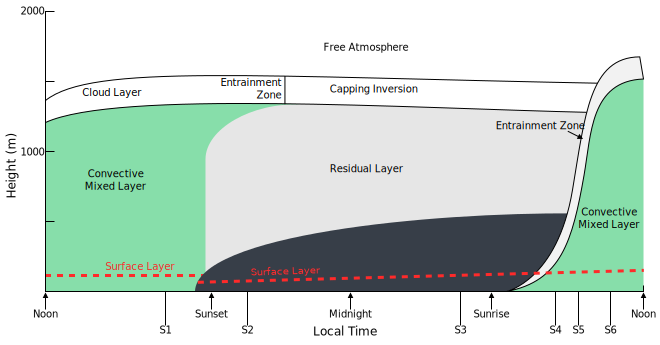
\includegraphics[width=0.8\linewidth]{chapter01/Atmospheric_boundary_layer.pdf}
    \caption{Évolution journalière schématique de la couche limite atmopshérique.
        Credit: By
        \href{https://commons.wikimedia.org/w/index.php?curid=18862904}{NikNaks} - Own
        work based on:
        \url{http://ars.sciencedirect.com/content/image/1-s2.0-S0360128504000371-gr4.jpg}.
        See also: \url{http://www.archaeocosmology.org/eng/tropospherelayers.htm}., CC
        BY-SA 3.0
    }%
    \label{fig:chapter01/Atmospheric_boundary_layer}
\end{figure}


\section{Les aérosols atmospheriques}%
\label{sec:les_aerosols_atmospheriques}
La nomenclature des aérosols est ainsi historiquement fondé sur leur taille:
\begin{itemize}
    \item \PMdix, dont le diamètre aérodynamique est inférieur ou égal à \SI{10}{\um} (petit
        grain de sable, pollens…)
    \item \PMdc, dont le diamètre aérodynamique est inférieur ou égal à \SI{2.5}{\um}
        (suie, fumée…)
    \item \PMun, parfois appellé aussi particules ultrafines (UFP), dont le diamètre
        aérodynamique est inférieur ou égal à \SI{1}{\um} (coagulation et condensation de
        vapeur…)
\end{itemize}


\subsection{Qu'est-ce qu'un aérosol?}%
\label{sub:quest-ce-quun-aerosol}

L'air que nous respirons est constitué majoritairement de gaz (\ce{N2}, \ce{O2}…) mais
également de particules solides ou liquides en suspension dans l'air. Ces particules, très
légères et de taille micrométriques ou moins, constituent une famille de composé appelé
communément particules fines, \textit{particulate matter} (PM) ou improprement particules
diesel dans le grand public.

Leurs tailles varient de quelques nanometres à plusieurs dizaines de micromètres.
À titre de comparaison, cela reviendrait à mettre dans la même catégorie une marche de
\SI{100}{m} pour aller chercher son pain à un voyage de \SI{10000}{km}.
Ainsi, cette nomenclature ''PM'' regroupe nécessairement des objets aux caractéristiques
très diverses, et comme le montre la Figure~\ref{fig:aerosolDistribution}, selon
que l'on observe les PM en s'intéressant à leur nombre, surface ou volume, l'importance
relative des classes de tailles change complètement.

\begin{figure}[ht]
    \centering
    \includegraphics[width=0.5\textwidth]{aerosolDistribution.pdf}
    \caption{Distribution \textbf{(a)} en nombre, \textbf{(b)} surface, et
        \textbf{(c)} volume, pour un ensemble typique de distribution trimodale
        d'aérosols. Figure adaptée du livre de~\textcite{seinfieldAtmospheric1998}.}
    \label{fig:aerosolDistribution}
\end{figure}

Ces différents modes reflètent différents procédés conduisant à leur présence dans l'air,
allant de la nucléation à partir de composé gazeux ou de source de combustion pour le mode
dit d'Aikten, le plus fin (prépondérant en nombre), permettant par coagulation d'atteindre
des particules plus grosses (mode d'accumulation), pour enfin, lorsque la vitesse de
coagulation est suffisante, atteindre le mode grossier, pouvant également être alimenté
par diverses autres sources comme la remise en suspension de poussière ou sable par le
vent, les pollens, les activités humaines, etc, comme nous le verons plus loin.

La nomenclature des aérosols est ainsi historiquement fondé sur leur taille:
\begin{itemize}
    \item \PMdix, dont le diamètre aérodynamique est inférieur ou égal à \SI{10}{\um} (petit
        grain de sable, pollens…)
    \item \PMdc, dont le diamètre aérodynamique est inférieur ou égal à \SI{2.5}{\um}
        (suie, fumée…)
    \item \PMun, parfois appellé aussi particules ultrafines (UFP), dont le diamètre
        aérodynamique est inférieur ou égal à \SI{1}{\um} (coagulation et condensation de
        vapeur…)
\end{itemize}


Ces catégories très diverses présentent ainsi des formes variées, comme illustré par les
clichés de microscopies électroniques présentés Figure~\ref{fig:micrography}. On retrouve
des particules sphériques de petites tailles, des formes plus géométriques issues de
processus de cristallisation comme le sel marin, etc.

\begin{figure}[ht]
    \centering
    \includegraphics[width=1.0\textwidth]{aerosol_micrographs.jpg}
    \caption{Image au microscope électronique à balayage, à des échelles différentes,
        illustrant la diversité de forme des aérosols.
        De gauche à droite : cendre volcanique, pollen, sel de mer et suie. Micrographies de
        l'USGS, UMBC (Chere Petty) et de l'Arizona State University (Peter Buseck). 
        Crédit : NASA earthobservatory \url{https://earthobservatory.nasa.gov/Features/Aerosols/}.
    }
    \label{fig:micrography}
\end{figure}

\subsection{Composition chimique}%
\label{ssub:composition_chimique}

En termes d'éléments constitutifs de ces PM, il est d'usage de regrouper les espèces en
différentes classes représentant les espèces majeures de la masse des PM. La
Figure~\ref{fig:chapter01/composition_chimique} présentes les gammes de concentrations
observée à travers le monde pour différentes typologies de site de prélèvement.
On y trouve différents ions issus de la condensation de la phase gazeuse (nitrate \NOt, formé à
partir des \ce{NO_x} et l'ammonium \ce{NH_4^+}, formé à partir de \ce{NH3}) et du sulfate
\SOq, formé par condensation du \ce{SO2} mais également émis par les volcans et les
activités anthropiques).
Une part également importante de la masse provient de la matière carbonée, notée ici
carbone organique (ou \textit{organic carbon} OC). Ce terme regroupe un nombre extrèmement
important d'espèce chimique comportant une chaine carbonée, de l'oxygène et
de l'azote. On y retrouve par exemple la cellulose ou autres sucres issues de sa
dégradation par combustion (lévoglucosan, mannosan, galactosan), des "polyols" (arabitol,
mannitol, etc) émis par les bactéries ou champignons~\autocite{samakePolyols2019}, ou encore
d'autres famille de molécule comme les alcanes, hopanes, composé aromatique polycyclique
ou même pesticide. Cette matière carbonée est souvent exprimée en terme de matière
organique (MO, ou \textit{organic matter} OM) prenant en compte la masse du carbone mais
également des autres atomes (oxygène, azote…) via un facteur correctif variant entre 1.2
et 2.3 suivant les lieux de prélèvement.
Mais le carbone est également présent sous forme plus "pure" (i.e. sans oxygène ni azote).
On parle alors de carbone élémentaire (\textit{elementary carbon} EC) lorsqu'il est mesuré
par méthode thermique, et de carbone noir (\textit{black carbon} BC) lorsqu'il est mesuré
par méthode optique. Cette distinction EC ou BC provient du fait qu'il existe un continuum
entre le carbone organique et le carbone élémentaire, et que chacune des méthodes
d'observation implique un seuil de différentiation entre les deux catégories.
Finalement, d'autres ions sont également présents, comme le sodium \ce{Na^+}, le chlore
\ce{Cl-}, le magnésium \ce{Mg^2+}, etc. mais également de nombreux éléments métalliques
comme le cuivre \ce{Cu}, l'aluminium \ce{Al}, le titan \ce{Ti}, le calcium \ce{Ca}, le fer
\ce{Fe}, etc.

La composition chimique d'un aérosol dépend de ses sources d'émissions (voir
également~\ref{sec:signature_chimique_des_sources_demissions} mais également des
différents processus bio-physico-chimiques présents dans l'atmosphère. En effet, sous
l'effet des radiations solaires, de la capacité oxydante de l'atmosphère ou des
micro-organismes vivant dans l'air, la composition chimique des aérosols évolue au cours
de sa vie. On parle d'\textit{aérosol primaire} lorsque la chimie reflète celle des
sources d'émission, et d'\textit{aérosol secondaire} lorsque les composés chimiques
proviennent de réactions ayant eu lieu dans l'air.

Cette sensibilité aux sources d'émissions explique en partie la variabilité observée sur
la composition chimique et sa sensibilité à la typologie du site d'étude. Les sites
marins présentant davantage de sels marins, les sites proches des déserts de sable
davantage de poussière minérale, les sites urbains davantage de marqueur de combustion
(EC), etc.

\begin{figure}[htpb]
    \centering
    \includegraphics[width=1.0\linewidth]{chapter01/composition_chimique.png}
    \caption{Composition chimique majeurs de la masse des \PMdix{} pour différentes
        typologies de sites de prélèvement. Crédit: \cite[figure 7.13]{boucherClouds2013},
        agrégeant 113 études sur au moins une année de prélèvement, entre 1993 et 2012.}%
    \label{fig:chapter01/composition_chimique}
\end{figure}

\subsection{Impacts des aérosols sur l'écosystème terrestre}%
\label{sub:impacts_des_aérosols_sur_l_écosystème_terrestre}

\subsubsection{Impacts climatiques}%
\label{ssub:impacts_climatiques}

Les aérosols sont des éléments essentiels de la machine climatique terrestre de part leur
interaction avec le rayonnement solaire et donc leur impact sur le bilan radiatif de la
Terre, mais également par leur interaction très forte avec la dynamique des nuages, au
point que les rapports du GIEC traitent dans le même chapitre les nuages et les aérosols.

\paragraph{Impact radiatif}%
\label{par:impact_radiatif}

De part leur faible taille, les aérosols diffusent le rayonnement incident et agissent donc
comme "bouclier thermique", ré-émettant une partie du flux solaire entrant dans l'espace,
conduisant ainsi à un refroidissement de l'atmosphère.
Cependant, les aérosols absorbent aussi une partie du rayonnement incident, augmentant
l'agitation thermique et donc conduisant à un réchauffement du climat.
Ces deux effets agissent de concert, à différentes altitudes de l'atmosphère, et selon la
composition chimique des aérosols.
Enfin, la déposition des aérosols, et notamment du black carbone, sur la neige ou les
glaces des banquises induit un effet bien connu de rétroaction positive : le carbone
absorbant le rayonnement normalement réémis par les surfaces blanches diminue l'albédo de
la surface, augmente localement la température, fait fondre la glace, découvrant des
surfaces plus sombre (roche ou océan), absorbant davantage de rayonnement, conduisant à
un réchauffement accru, etc.

\paragraph{Noyaux de condensation des nuages}%
\label{par:noyaux_de_condensation_des_nuages}

Mais les aérosols, grâce à leur taille et leurs ions, permettent également de baisser
l'énergie d'activation nécessaire à l'agrégation de la vapeur d'eau sous forme liquide en
gouttelettes, puis goutte, facilitant l'apparition des nuages. Ainsi, les aérosols agissent
comme noyaux de condensation des nuages (CCN pour \textit{cloud condensation nuclei}). Or
les nuages empêchent certes les infrarouges terrestres de repartir vers l'espace, mais
présentent également un albédo élevé, renvoyant une grande partie du rayonnement à courte
longueur d'onde du soleil vers l'espace. L'effet observé est donc un refroidissement du
climat.
Aussi, pour une même quantité d'eau, le nombre de CCN disponible conditionne la taille des
gouttelettes des nuages, et donc leur taille, durée de vie et probabilité de se
transformer en nuage précipitant.

\paragraph{Impacts sur le dérèglement climatique en cours}%
\label{par:impacts_sur_le_dereglement_climatique_en_cours}

Pour ces différents aspects, très brièvement exprimé ici, l'impact total des aérosols sur
le climat est connu avec une incertitude élevée. 

Notamment, leur contribution à la différence du forçage radiatif entre 1750 et 2011 --qui
est de \SI{2.29}{\W\m\squared}-- s'estime entre
\SIrange[range-phrase=~et~]{-0.77}{0.23}{\W\per\m\squared}, avec un forçage négatif pour
les poussières minérales, le sulfate, nitrate et carbone organique, mais positif pour le
carbonne noir.  Quant à leur rôle sur la dynamique des nuages, il s'estime entre
\SIrange[range-phrase=~et~]{-1.33}{-0.06}{\W\per\m\squared}, mais présente des
incertitudes plus élevés dû fait de la complexité à prendre en compte ces phénomènes dans
les modèles de climat. C'est actuellement le forçage radiatif le moins bien connu de la
machine climatique Terrestre.

\subsubsection{Impacts environnementaux}%
\label{ssub:impacts_environnementaux}

La durée de vie des aérosols dans l'atmosphère entre leur émission et leur déposition est
de plusieurs jours. Dans ce délai, la circulation atmosphérique les déplacant sur des
distances pouvant être de plusieurs milier de kilomètre. Il n'est pas rare par exemple en
Europe d'avoir des épisodes de dépositions de sable provenant du désert saharien. Ce
déplacement longue distance d'aérosols est même un des mécanismes clef de certains "bloom"
de phytoplancton, apportant d'importante quantité de nutriment à la surface de l'océan (en
métaux et phosphate notamment).
Plus spectaculaire, les cendres volcaniques relarguées dans l'atmosphère suite à de
violentes éruptions, en plus de leur impact climatique potentiel, peuvent occasioner des
pluies acides du fait de la présence en quantité de sulfate dans ces cendres.
Autre exemple marquant, le nitrate est l'un des éléments limitant de la croissance des
plantes en prairie d'altitude. Or une partie importante de ce nitrate est apporté par
déposition de nitrate d'amonium particulaire provenant du transport longue distance.

Cette liste n'a pas pour but d'être exhaustif mais uniquement de présenter à quel point
les aérosols et leur composition chimique variée impacte directement de nombreux
écosystèmes terrestres, qu'ils proviennent de sources anthropiques comme c'est le cas pour le
nitrate, ou de sources naturelles.

\subsection{Impacts sanitaires}%
\label{sub:impacts_sanitaires}

Finalement, l'impact sanitaire des aérosols sur la population humaine a commencé à être
un sujet de recherche suite à l'industrialisation et aux épisodes de "smog" causant la
mort de plusieurs personnes à Engis (Meuse, Belgique) en 1930, Donora (Pennsilvanie, USA)
en 1948 ou encore le plus connu "Great smog of London", en 1952. Durant ces épisodes de
pollutions, il est important de noter que la sur-mortalité due à l'exposition aigue
durant l'épisode de pollution est très importante (jusqu'à 3 fois supérieure à la normale
pour le smog de Londres), mais que la surmortalité persiste dans les mois qui suivent
--pendant près d'un an pour le smog de Londres, alors même que les niveaux de pollutions
étaient revenus à leurs états pré-décembre 1952 \autocite{bellReassessment2001}.  Ces
épisodes de pollutions intenses marquent le début de la prise de conscience par la
population de la problématique de la pollution de l'air et ont conduit à la première
législation anglaise en matière de qualité de l'air en 1956 avec le \textit{Clean Air
Act}. Aussi, des programmes de mesures de la qualité de l'air pour différents polluants
ont émergés et les actions misent en œuvre au niveau national et international ont permis
en Europe une amélioration très sensible de la qualité de l'air
(Figure~\ref{fig:chapter01/tendance_polluants}).

\begin{figure}[ht]
    \centering
    \includegraphics[width=0.9\linewidth]{chapter01/tendance_polluants.pdf}
    \caption{Évolution temporelle des émissions cumulés des 28 pays de la zone européenne
    depuis 1990, indiquant une prise de conscience et une diminution des émissions de
différents polluants gazeux (SOx et NOx) et particulaires (\PMdix{} et \PMdc). Données
issues de \textit{National emissions reported to the Convention on Long-range
Transboundary Air Pollution (LRTAP Convention)}, ©European Environment Agency (EEA).}%
\label{fig:chapter01/tendance_polluants}
\end{figure}


Cependant, la qualité de l'air (incluant les aérosols, mais également les
composés gazeux comme les \ce{NO_x} ou l'ozone) demeure actuellement la 5\ieme{} cause de
mortalité dans le monde, représente un décés sur dix et est catégorisé "cancérogène
certain" par le CIRC depuis 2013. En Europe, pour l'année 2013, c'est
ainsi \num{800000} personne qui sont décédés des suites de maladies cardiovasculaires,
cancer, pneumonie… directement attribuable à la qualité de l'air
\autocite{worldhealthorganizationAmbient2016}. Récemment, \textcite{lelieveldLoss2020}
estiment qu'en moyenne et à travers le monde, c'est 2.9 ans de vie perdue par personne
qui sont imputables à la pollution de l'air, dont 1.7 ans "évitables" car provenant
directement de sources anthropiques.

En termes de bilan financier, la banque mondiale en collaboration avec l'Institute for
Health Metrics and Evaluation (IHME) de l'université de Washington estimait que le coût
associé aux décés prématurés de la seule année 2013 s'évaluait à plus de \$5.11 trillions
de dollar dans le monde~\autocite{worldbankCost2016}.

Afin de limiter cet impact sanitaire, de nombreux pays ont définis des seuils de
concentrations de différents composés (voir Tableau~\ref{tab:seuil_PM} pour les PM).
Seulement ces seuils sont différents d'une institution à une autre. Par exemple, entre
2015 et 2017, le seuil de concentration journalière recommandé pour les \PMdix{} par
l'union européenne (\SI{50}{\ugm} en moyenne journalière) était dépassé pour entre 13 et
19~\% de la population européenne, mais cette proportion augmente à entre 42 et 62~\% si
l'on prend en compte le seuil recommandé de l'OMS de \SI{20}{\ugm} en moyenne
annuelle~\autocite{europeanenvironmentagencyAir2019}.  De plus, il est à noter qu'il
n'existe pas de seuil à partir duquel l'exposition aux PM est inoffensif.

\begin{table}[ht]
    \begin{ThreePartTable}
        \centering
        \caption{Seuils de concentration de PM recommandés par différents organismes.}
        \label{tab:seuil_PM}
        \begin{tabular}{ccSc}
            \toprule
            Organisme       & Polluant & {Concentration (\si{\ugm})} & Période \\
            \midrule
            OMS\tnote{a}    & \PMdc  & 10 & moyenne annuelle       \\
            OMS\tnote{a}    & \PMdc  & 25 & moyenne sur \SI{24}{h} \\
            OMS\tnote{a}    & \PMdix & 20 & moyenne annuelle       \\
            OMS\tnote{a}    & \PMdix & 50 & moyenne sur \SI{24}{h} \\
            Europe\tnote{b} & \PMdc  & 25 & moyenne annuelle       \\
            Europe\tnote{b} & \PMdc  & 20 & moyenne sur 3 ans      \\
            Europe\tnote{b} & \PMdix & 40 & moyenne annuelle       \\
            Europe\tnote{b} & \PMdix & 50 & moyenne sur \SI{24}{h} \\
            France\tnote{c} & \PMdc  & 25 & moyenne annuelle \\
            France\tnote{c} & \PMdix & 50 & moyenne sur \SI{24}{h} (\SI{<35}{jour\per an}) \\
            France\tnote{c} & \PMdix & 40 & moyenne annuelle \\
            \bottomrule
        \end{tabular}
        \begin{tablenotes}
        \item[a] OMS air quality guideline \cite{worldhealthorganizationWHO2006}
        \item[b] Directive 2008/50/EC \cite{officialjournaloftheeuropeanunionDirective2008}
        \end{tablenotes}
    \end{ThreePartTable}
\end{table}

\section{Détermination des sources d'émission des PM}%
\label{sec:source_apportionment_of_pm}

Comme nous l'avons vu, les sources d'aérosols sont très diverses.
Afin de pouvoir avoir un impact sur les concentrations de polluants, il est primordial de
retracer leur provenance. Plusieurs techniques d'analyses existe, qu'elles soient purement
physiques ou géochimiques.

\subsection{Signature chimique des sources d'émissions}%
\label{sec:signature_chimique_des_sources_demissions}

Chaque source d'émission n'émettant pas les mêmes composés, une analyse chimique
des PM permet l'estimation des contributions des différentes sources aux PM observés.
Seulement, il n'est pas possible de mesurer l'entièreté des plus de 1000 espèces chimiques présentes
dans les aérosols.
Il convient donc de connaître au mieux la signature chimique des différentes sources
d'émissions, notamment via des prélèvements à l'émission en condition
réelle ou en chambre d'étude. La connaissance des espèces spécifiquement émises ou des
ratios d'émissions entre différentes espèces des différentes sources permetront par la
suite l'attribution de la contribution de ces sources aux PM observés.

\subsubsection{Analyse chimique des particules fines}%
\label{ssub:analyse_chimique_des_particules_fines}

Les données utilisées pour cette thèse proviennent d'analyse faite en laboratoire à
partir de prélèvement de terrain (mesure \textit{off-line}) via des préleveurs
automatiques haut-volume, selon les recommandations de
l'EN~16450:2017~\autocite{cenAmbient2017a}, chaque prélèvement correspondant à une
journée d'échantillage. Les prélèvements étant réalisé sur des filtres en fibre de quartz
pré-chauffée, grâce à un préleveur haut-débit (\SI{30}{\cubic\m\per\hour}) DA80 digitel.
La fraction prélevée correspond toujours aux \PMdix{}.

Dans les espèces couramment analysés et utilisés durant cette thèse, on retrouve :

\begin{description}
    \item[OC et EC] le carbone organique et élémentaire, mesuré par méthode
        thermo-optique~\autocite[Sunset Lab. Analyser]{birchElemental1996}, par le
        protocole EUSAAR-2~\autocite{cavalliStandardised2010,cenAmbient2017a};

    \item[Ions] \ce{Cl-}, \ce{NO3^-}, \ce{SO4^2-}, \ce{NH4+}, \ce{Na+}, \ce{K+},
        \ce{Mg^2+}, \ce{Ca^2+} et acide méthane suflonique (MSA), déterminés par
        chromatographie ionique~\autocite{jaffrezoSeasonal2005,cenAmbient2017b};

    \item[Métaux et éléments traces] Al, Ag, As, Ba, Be, Br, Bi, Ca, Cd, Ce, Co, Cr, Cs,
        Cu, Fe, K, La, Li, Mg, Mn, Mo, Na, Ni, Pb, Pd, Pt, Rb, Sb, Sc, Se, Sn, Sr, Ti, V,
        Zn et Zr, mesurés par ICP-AES ou
        ICP-MS~\autocite{allemanPM102010,mbengueSizedistributed2014,cenAmbient2005}

    \item[Monosacharides] Levoglucosan, mannosan, galactosan, arabitol, manitol, sorbitol
        et glucose, analysés par
        HPLC-PAD~\autocite{piotQuantification2012,wakedSource2014}.

\end{description}

\subsubsection{Profile chimique des sources d'émissions courantes}%
\label{ssub:profile_chimique_des_sources_d_émissions_courantes}

\begin{description}
    \item[Combustion de biomasse] provenant en Europe majoritairement du chauffage
        domestique. Le type de combustible et les conditions de combustion influence
        grandement sur les espèces chimiques émises. On retrouve cependant toujours de
        l'OC en grande quantité, ainsi que de l'EC. Aussi, si le BC est mesuré, il est
        possible d'estimer la part du BC provenant de cette source de combustion \BCwb{}
        (\textit{BC wood burning}).
        Provennant de la pyrolyse de la cellulose, le lévoglucosan, mannosan et
        galactosan forment 3 proxy spécifique de cette source, car il n'existe pas d'autre
        procédé connu conduisant à leur présence dans l'atmosphère que la combustion de
        bois~\autocite{jordanLevoglucosan2006,puxbaumLevoglucosan2007}.
        Enfin, du potassium \ce{K+} et du rubidium Rb sont également associés à cette
        source~\autocite{navaBiomass2015,gollyEtude2014,chevrierChauffage2016}.

    \item[Traffic routier] émettant différents métaux (Ca, Cu, Mo, Pb, Sb, Sn, Fe, Zr,
        Ti) et de la matière carbonée --notamment de l'EC-- et des composés organiques
        (hopanes, alcanes)~\autocite{schauerCharacterization2006,charronIdentification2019}. Les émissions
        véhiculaires sont parfois séparées en 2 sous-types : émissions à l'échappement
        provenant de la combustion~\autocite{allenSize2001,huMetals2009,vianaSource2008},
        et émissions hors-échappement (abrasion de la route, usure des freins et pneus,
        etc.)~\autocite{grigoratosBrake2015,sandersAirborne2003,sternbeckMetal2002}.

    \item[Émission primaire biogénique] directement émise par les micro-organismes du sol
        et des plantes, qui, de par leur activité biologique, émettent notamment
        différents polyols : arabitol, mannitol,
        sorbitol~\autocite{bauerSignificant2008,yttriAmbient2007,samakePolyols2019}.

    \item[Poussière crustale] remise en suspension par le vent ou les activités humaines
        (mine, carrière, etc). Ce profil chimique reflète celui de la croute continentale
        et présente donc du \ce{Mg^2+}, \ce{Ca^2+}, Ti, Mn et Fe, mais très peu de composés
        organiques~\autocite{almeidaSource2005,dallostoHourly2013,morenoVariations2011,putaudSizesegregated2004}.

    \item[Sel de mer] issue des embruns marins, présentant donc une grande proportion de
        \ce{Na+} et \ce{Cl-}, mais également de
        \ce{Mg^2+}~\autocite{belisCritical2013,odowdMarine1997,pioClimatology2007}. Il
        est à noter que le sel de route, notamment en vallées alpines, présente la même
        composition chimique~\autocite{airrhone-alpesInfluence2012}.

    \item[Industrie] Les profils chimiques des sources industrielles sont très variables
        car dépendent directement du type d'industrie. Cependant, il est courrant d'y
        retrouver des métaux, du \SOq et certains composés organiques spécifiques (HAP et
        HAPs, hopanes...) selon les procédés
        industriels~\autocite{sylvestreComprehensive2017}.

    \item[Port et bateau] proche des côtes notamment. Marqué par la présence de V et Ni,
        provenant de la combustion de fuel lourd, mais également de composés organiques
        comme les hopanes.

    \item[Agriculture] émetant notamment du nitrate et de l'ammoniac à travers les
        fertilisants de synthèse ou de fumier. Cette source d'émission est notamment
        responsable des pics de pollution printanier, lors des épandages agricole à cette
        période.

    \item[Volcan] beaucoup plus ponctuel --surtout en Europe-- mais néanmoins possible
        (par exemple l'Eyjafjöll en 2010), les volcans émettent de grande quantité de
        poussère minérale et d'éléments traces, mais également de soufre et donc de \SOq.

\end{description}

\subsubsection{"Sources" ou processus secondaires}%
\label{ssub:_sources_secondaires}

Aux sources primaires précédemment listées, il faut ajouter les processus secondaires liés
à la photochimie ou au vieillissement des aérosols, qui conduisent à la formation de
nouvelles espèces chimiques.

\paragraph{Aérosol organique secondaire}%
\label{par:aérosol_organique_secondaire}

Notamment, la biologie est connue pour émettre du dimethyl sulfate (DMS), s'oxydant en
MSA dans l'atmosphère. Sa présence dans les PM trace donc le vieillissement d'un aérosol
d'origine organique.  L'oxalate est également un composé issu de réaction photochimique,
mais la diversité des composés primaires et voie de réaction rend extrêmement difficile
l'identification de la source originelle.
On nomme alors ces aérosols \textit{secondary organic aerosol} (SOA), dont le
dénominateur commun est de présenter une fraction importante de matière organique
oxygéné. Il est compliqué avec des analyses moléculaires d'en déterminer l'origine et des
travaux sont en cours en ce sens et présenté dans le chapitre~\ref{chap:todo}.

Il faut noter que d'autres techniques d'analyses, notamment l'ACSM, permettent une
analyse plus avancée de cette fraction organique de l'aérosol, sans pour autant pouvoir
caractériser moléculairement les éléments retrouvés.

\paragraph{Aérosols inorganique secondaire}%
\label{par:aérosols_inorganique_secondaire}

Mais la partie organique n'est pas la seule à réagire dans l'atmopshère. Ainsi, les NOx,
gazeux, émis notamment par le transport routier, peuvent condensés en phase particulaire
lorsqu'ils s'associent à l'ammoniac, provenant du secteur agricole, pour former du
nitrate d'ammonium \ce{NO3NH4}. Il en est de même pour le \ce{SO2} émis par différentes
sources ou des fonctions sulfatés de la matière organique, et l'ammoniac, condensant en
sulfate d'ammonium \ce{SO4(NH4)2}.

\paragraph{Vieillissement et volatilité}%
\label{par:vieillissement_et_volatilité}

Aussi, la partie la plus volatile de la phase particulaire tend à s'évaporer et rejoindre
la phase gaseuse au cours du temps. C'est ainsi qu'après plusieurs jours de transport
dans l'atmosphère, le sel de mer peut avoir ''dégazer'' le chlore présent dans son réseau
cristallin, et présenté des substitutions avec du sulfate ou du nitrate. De même que la
sodium peut avoir été remplacé par d'autres cations comme le potassium ou le magnésium.
Souvent, ce procédé est associé a une augmentation de la matière organique liée à cet
aérosol.

\subsection{Modèle d'attribution des sources}%
\label{sec:source_apportionment_model}

Afin d'estimer la contribution de chaque sources de PM à un point donnée, il est possible
d'utiliser 2 grandes familles de modèles d'attribution des sources (\textit{source
apportionment} (SA)). La première est fondée sur notre connaissance des
émissions et de la météorologie et calcul les réactions physico-chimiques depuis les
sources jusqu'au lieu d'étude (modèle dit de chimie-transport (\textit{chemical transport
model} (CTM)) alors que la deuxième s'évertue à mesurer en un point donné
la chimie des PM et par traitement statistique, attribue a différente source ou
''facteur'' leur contribution aux concentrations observées (modèle dit récepteur
(\textit{receptor model} RM)).

\subsubsection{Modèle déterministe de chimie-transport}%
\label{ssub:modele_deterministe_de_chimietransport}

\paragraph{Présentation}%
\label{par:presentation}

Les modèles déterministes s'appuient sur l'inventaire des sources d'émissions sur la
région étudiée. Ces cadastres d'émissions sont regroupés en catégorie \textit{Selected
Nomenclature for reporting of Air Pollutants} (SNAP) représentant chacune un secteur
d'activité : Énergie, Procédés industriel, Agriculture, Déchets, Autres et enfin
Naturelle.
Chacune de ces catégories possèdant évidemment des sous-catégories raffinant la
classification (par exemple, les émissions de l'aviation civile de plus de \SI{100}{m} de
long se retrouvent dans le SNAP 080503 (ou \textit{Nomenclature For Reporting} (NFR)
1.3.A.c) autrement dit Énergie - Combustion - Aviation - Aviation civile de plus de
\SI{100}{m})~\autocite{europeanenvironmentagencyEMEP2019}.
À chacun de ces SNAP est associé un profile d'émission (\ce{O3}, \ce{SO2}, NOx, \ce{NH3}, \PMdix, \PMdc,
VOC principalement).

Vient ensuite un inventaire de ces sources d'émissions sous forme de cadastre géographique
et temporelle. Notamment la \textit{Convention on Long-Range Transboundary Air
Pollution} (LRTAP) implémenté par l'\textit{European Monitoring and Evaluation Program}
(EMEP) sous l'égide de \textit{United Nations Economic Commission for Europe} (UNECE),
prévoit que les différentes parties prenante à cette convention présentent un rapport de
leurs émissions régulièrement à l'EMEP.

Il est alors possible de construire des modèles déterministes de dispersion et de
réaction des polluants, en couplant un modèle de diffusion résolvant les équations de la
physique de l'atmosphère (navier-stoke, turbulence, rayonnement, etc) avec un modèle
physico-chimique faisant évoluer les composés gazeux et particulaires, incluant leurs
émissions, dépôts, interaction physico-chimique, etc. Pour n'en citer que quelqu'uns : 
Community Multi-scale Air Quality (CMAQ)\footnote{CMAQ: \url{https://www.epa.gov/cmaq}},
Comprehensive Air Quality Model with Extensions (CAMx)\footnote{CMAx : \url{http://www.camx.com/}},
WRF-Chem\footnote{WRF-chem : \url{https://www2.acom.ucar.edu/wrf-chem}},
Chimère,
LOTOS-EUROS...

La raison de la pluralité de ces modèles provient des différentes paramétrisations
possibles des équations physiques, mais également des choix conceptuels de recherche.

\paragraph{Source apportionment}%
\label{par:source_apportionment}

Concernant l'attribution des sources, il est possible d'utiliser deux techniques au sein
des CTM:

\begin{enumerate}
    \item Faire une première simulation incluant toutes les sources d'émissions, puis une
        deuxième avec une source en moins. La différence reflétant l'impacte de la source
        supprimée sur les concentrations ambiantes ;
    \item Tracer la provenance de chacunes espèces chimiques lors des schémas réactionnels
        (\textit{source labelling} ou \textit{tagged species}).
\end{enumerate}

Seulement, du fait des nombreux processus non linéaires, la suppression d'une source
d'émission aura des répercussions beaucoup plus complexe que la simple diminution des
concentrations propre à cette source (par exemple, des NOx pourraient ne pas passer en
phase particulaire du fait d'un manque d'ammoniac). La première solution correspond donc à
se demander 
\begin{quote}
    Si les émissions de cette source sont diminuée ou supprimée, quels impacts cela va-t-il
    avoir sur les concentrations finales ?
\end{quote}
alors que la deuxième répond à
\begin{quote}
    Dans la concentration ambiante de PM, à combien s'estime la contribution de cette source
    d'émission ?
\end{quote}
Cette dernière technique a commencé été implémenté plus récemment dans certains
CTM~\autocite{wangDevelopment2009,wagstromDevelopment2008,kranenburgSource2013,brandtContribution2013}
et détaillé dans le rapport de~\textcite{mirceaEuropean2020}.

Cependant l'utilisation des CTM présente certaines limites du fait de leur complexité.
Notamment, il semble illusoire de pouvoir un jour inclure toutes les réactions chimiques
possibles dans les modèles déterministes, et quand bien même ce serait le cas --car les
modèles réactionnels sont de plus en plus poussées--, il faudrait alors avoir des
inventaires d'émissions beaucoup plus complet et précis temporellement, avec aucune
certitude d'un oubli potentiel d'une source non prise en compte.  Aussi, la limitation
physique des modèles météorologiques se retrouvent dans les CTM. Il est donc compliqué
d'envisager, du fait du coût de calcul et de stockage, une simulation à \SI{10}{m} de
résolution spatiale (ou moins), ce qui serait cependant nécessaire pour appréhender
correctement des phénomènes précis, comme les inversions thermiques des vallées alpines.

\subsubsection{Modèles récepteurs}%
\label{ssub:model_recepteur}

À l'inverse, il est possible d'estimer les sources contribuant aux concentrations
ambiantes en un lieu donné sans la moindre information météorologique ou simulation
déterministe. Pour cela, il convient de faire des prélèvements sur le lieu d'étude,
d'analyser la chimie que l'on y trouve, et à l'aide de modèle statistique, de retrouver
les différents profils de source et leur contribution, traduisible pas l'équation
d'équilibre des masses
\begin{align}
    \label{eq:mass_balance}
    X &= G \cdot F
\end{align}
où $X$ est la matrice de dimension $n\times m$ des observations, $G$ est la matrice des
contributions de taille $n\times p$ et $F$ la matrice des profils de taille $p \times n$,
avec $n$ le nombre d'échantillon, $m$ le nombre de variables chimiques mesurées et $p$ le
nombre de facteur. Un facteur peut être une source d'émission (combustion de biomasse par
exemple), mais également regrouper des espèces chimiques provenant d'un même processus
secondaire (nitrate d'ammonium par exemple).
Il est courrant d'exprimer $X$ en \si{\ugm}, $G$ en \si{\ugm} ou concentration
normalisée~\si{[-]} et $F$ en \si{\micro\g\per\micro\g} ou \si{\ugm}.

Si l'on mesure $X$, ce qui nous intéresse ici est de connaître $G$ et/ou $F$. Si l'on
admet que l'on connait a priori les profils d'émissionis possibles, alors $F$ est connu, et
l'on cherche à estimer $G$. Le modèle de déconvolution adapté est alors le
\textit{Chemical Mass Balance} (CMB). À l'opposé, on peut n'avoir aucune information a
priori à la fois sur les contributions et les profils d'émissions. On utilisera alors le
modèle de déconvolution \textit{Positive Matrix Factorization} (PMF).  Ces 2 types de
modèles statistiques sont aux deux extrêmes d'un spectre de modèle de déconvolution depuis une
information ''absolue'' des profils de sources à une absence totale d'information de ces
mêmes profils.  Il existe cependant un continuum entre ces deux pôles (voir
Figure~\ref{fig:chapter01/source_apportionment_methods}), et de nombreux modèles ont été
développés et améliorés depuis la première étude de SA de \textcite{colucciAutomotive1965}
utilisant la ''simple'' corrélation entre le \ce{CO} et le plomb et benzo(a)pyrène.  Une
revue détaillée et historique du fonctionnement de ces différents modèles peut-être
retrouvées dans les articles de
\textcite{henryHistory1997,vianaSource2008,belisCritical2013,hopkeReview2016}.

\begin{figure}[ht]
    \centering
    \includegraphics[width=0.6\linewidth]{chapter01/source_apportionment_methods.png}
    \caption{
        Connaissance a priori nécessaire pour les différents modèles de SA existant,
        depuis la simple analyse de facteur par ACP au modèle CMB. Crédit :
        \textcite{vianaSource2008} adaptée de \textcite{schauerCharacterization2006}
    }%
    \label{fig:chapter01/source_apportionment_methods}
\end{figure}

Dans cette thèse, seul le modèle PMF résolue grâce au solver ME-2 développé par
\textcite{paateroMultilinear1999} a été utilisé, et va maintenant être décrit en détail.

\subsubsection{Modèle source récepteur PMF}%
\label{ssub:pmf}

\paragraph{Formulation mathématique}%
\label{par:formulation_mathématique}

Le principe de la PMF provient initialement de la recherche sur le \textit{machine
learning}, et plus particulièrement de l'analyse factorielle appliqué au problème
bilinéaire $X=G\times F$. L'intérêt initial étant de permettre une réduction
dimensionnelle sans perte d'information. Par exemple, en informatique, une image de $n$
par $m$ pixels forme une matrice $n\times m$ éléments. S'il est possible de retrouver
cette matrice par multiplication de 2 matrices $G$ ($n\times p$) et $F$ ($p \times m$),
alors la quantité d'information stockée dans $G$ et $F$ est $n
\times p + p \times m = p \times (n + m)$. Ainsi, tant que $p < \frac{n\times m}{n+m}$,
alors le nombre d'éléments de $G\times F$ est toujours inférieur au nombre d'élément de
$X$, permettant un gain de mémoire de plus en plus important au fur et à mesure que $n$ et
$m$ augmente.
Tout le problème réside en le fait de trouver la décomposition de $X$ en minimisant
l'erreure engendrée par cette simplification.

Aussi, on observe que la formulation $X = G\cdot F$ est similaire à celle de
la conservation de la masse (Eq.~\ref{eq:mass_balance}). Ce problème peut-être résolu par
analyse en composante principale (ACP), seulement, le résultat obtenu présente des
combinaisons linéaire (additive et soustractive) des différents composants. Cette possible
négativité des composants n'a pas de sens dans beaucoup de domaine physique, y compris en
géochimie. \textcite{paateroPositive1994} présente donc une nouvelle méthode de
déconvolution, implémentant une contrainte de non-négativité, nommée \textit{Positive Matrix
Factorization} (PMF). 

La formulation est la suivante : étant donné une matrice d'obervation $X$ de taille
$n\times m$, une matrice associée des incertitudes $U$ de taille $n \times m$ et un rang
$p$, alors 
\begin{align}
    \label{eq:pmf_formulation}
    X &= G \cdot F + E \\
    \forall i,k,j &, G_{ik}\geq 0 \text{ et } F_{kj}\geq 0\\
    Q &= \sum_{i=1}^n\sum_{j=1}^m E_{ij}^2/U_{ij}^2\\
    {Q, F} &= \argmin_{G,F} Q.
\end{align}

Différent algorithme de résolution du système Eq.~\ref{eq:pmf_formulation} ont été développés.
L'implémentation initiale de~\textcite{paateroLeast1997} a été amélioré pour pouvoir
ajouter des contraintes sur les matrices $G$ et $F$, notamment grâce au solveur
\textit{multi-linear engine} (ME-2) \autocite{paateroMultilinear1999}. En effet, il
n'existe pas de solution unique au problème Eq.~\ref{eq:pmf_formulation}, notamment, car le
système est invariant par rotation:
\begin{align}
    \label{eq:rotationalambiguity}
    X   &= G \cdot F + E \\
        &= (G \cdot T) \cdot (T^{-1} \cdot F) + E\\
        &= G' \cdot F' + E
\end{align}
et ainsi une infinité de solution coexistent. Pour estimer, et limiter, cette ambiguité
rotationelle, le ME-2 permet notamment l'ajout de contrainte sur les matrices $G$ et $F$,
limitant de fait le nombre de rotation possible de ces matrices.

\paragraph{Interprétabilité du modèle PMF}%
\label{par:interpretabilite_du_model_PMF}

L'avantage de la PMF réside en le fait que l'algorithme n'est pas fondé sur la
correlation entre variable, comme c'est le cas de l'ACP, mais bien en la formation d'un
modèle additif linéaire de ce qui est observé.
\begin{quote}
    We shall not be satisfied in finding some correlations, we wish to form a quantitative
    model of what was observed! \autocite{paateroPositive1994}
\end{quote}

Il a été montré que la PMF est capable d'extraire des informations partielles cohérentes des
données là où l'ACP n'est qu'une représentation holistique~\autocite{leeLearning1999}. Par
exemple, appliquée à la reconnaissance d'image faciale, la PMF déconvolu les visages en
sous partie (bouche, sourcils, front, etc) alors que d'autres méthodes ''se contentent''
d'une approche globale de l'information et où seules les premières dimensions portent
l'information nécessaire à la reconstruction du signale (voir
figure~\ref{fig:chapter01/NMFvsPCA}).

\begin{figure}[ht]
    \centering
    \includegraphics[width=1.0\linewidth]{chapter01/NMFvsPCA.png}
    \caption{Analyse factorielle par PMF (i.e. NMF for \textit{non-negative matrix
    factorization}) et ACP d'une banque d'image de 2429 images en niveau de gris de 19
    pixel par 19 pixels. Les deux techniques essaient de reproduire l'image originale en
    fonction de leur apprentissage.
    \textbf{A)} Le rang de la PMF est $p=49$, correspondant aux 49
    représentations des $19\times19$ images à gauche, chacune étant un facteur de la
    matrice $F$, et leurs ''contributions'' respectivement identifiées par le carré de 7 par
    7 en niveau de gris, à droite.
    \textbf{B)} Analyse en composante principale, le carré de gauche représentant les 49
    vecteur propres et celui de droite les 49 valeurs propres.
    Les échelles de couleurs sont : rouges pour les coefficients négatifs, noirs pour les
    coefficients positifs.
    Figure adaptée de \textcite{leeLearning1999}}%
    \label{fig:chapter01/NMFvsPCA}
\end{figure}

\paragraph{Applicabilité en science de l'atmosphère}%
\label{par:applicabilité_en_science_de_l_atmosphère}

Dans le cas qui nous intéresse ici, cela signifie que chacun des vecteurs de la matrice
$F$ correspond à un profile d'emission, en \si{\ugm}, indépendant des autres profils, et
que la matrice $G$ représente la contribution de chacun de ces profils au jour
considéré, de manière cohérente avec l'équation de conservation de la masse.

L'application du modèle PMF a été utilisé de nombreuse fois, et a été grandement favorisé
par son implémentation dans le logiciel de l'EPA: EPA PMF5.0~\autocite{norrisEPA2014}.
Si l'EPAPMF5 est massivement utilisé pour les données provenant d'analyse de
filtre, l'utilisation de spectre de masse provenant de mesure d'AMS est facilité par
l'utilisation du logiciel SoFi~\autocite{canonacoSoFi2013}. Ces deux logiciels utilisent
le solveur ME-2 pour résoudre le système d'équation de la PMF.

\paragraph{Subjectivité de l'expérimentateur}%
\label{par:subjectivité_de_l_expérimentateur}

L'utilisateur a donc 3 paramètres à choisir manuellement : les observations $X$, leurs
incertitudes $U$ et le nombre de facteur (ou rang) $p$. Chacuns de ces paramètres
influencera la solution finale obtenue et provient de la subjectivité de l'expérimentateur:
quelles espèces chimiques utiliser ? garder ou non ce jour d'observation ''extrême'' ?
quelles incertitudes pour quelles espèces ? combien de facteur utiliser ?

Une inter-comparaison de modèle récepteur sur le site de Lens a été conduit par
\textcite{belisEvaluation2020}. Les 38 études des participants bénéficiaient de
la même base de donnée et non seulement le nombre de facteur retrouvé varie de 5 à 12 mais 
le contributions temporelles, bien que globalement concordante, varient entre les
différentes études, comme le montre les z-scores de la figure~\ref{fig:chapter01/belisEvaluation2020_fig2a}
\footnote{Le z-score représente ici une distance entre les contributions temporelles de
    chacune des sources des différentes études à la moyenne de celles-ci, définie par 
    \begin{align}
        \label{eq:z-score}
        z = \frac{x-X}{\sigma}
    \end{align}
    où $x$ est une série temporelle d'un facteur, $X$ la moyenne des séries temporelles de
    ce facteur issue des différentes études et $\sigma$ définie comme $0.5\times X$
    \parencite{pernigottiDeltaSA2018}.
}.

Cette diversité s'explique par le \textbf{choix des variables utilisées par la PMF}, reposant au
final sur la ''connaissance d'expert'' de l'expérimentateur. En effet, toutes les données
d'entrée ne portent pas la même quantité information et l'ajout d'espèces traceuses de
sources particulières conduira à l'obtention d'un facteur relié à cette source. Au
contraire, l'ajout trop important d'espèce n'apportant pas suffisamment d'information peut
déstabiliser statistiquement le modèle et résulter en une solution statistiquement faible
(peu de répétabilité, variance importante, etc) et de fait géo-chimiquement douteuse.
Aussi, le \textbf{choix des contraintes} à appliquer impliquera des solutions
nécessairement différentes. Là encore, ces contraintes sont issues de la connaissance a
priori de l'expérimentateur et sont donc en partie subjective.

Enfin, l'identification des facteurs est laissé à l'appréciation de l'expérimentateur. Il
faut donc savoir identifier quel profil d'émission peut être responsable du facteur
observé. Cette nomenclature des facteurs est elle aussi subjectif et non standardisée :
véhiculaire, émission routière, trafic routier, combustion diesel, etc. peuvent être
différent nom donné au même profil, par différents utilisateurs.
Des travaux récents, portés par le groupe FAIRMODE du JRC, portent notamment sur une
harmonisation de cette nomenclature, à travers la construction d'une donnée européenne de
profil de source standardisée et hierarchisé : SPECIEUROPE~\autocite{pernigottiSPECIEUROPE2016}.

Pour toutes ces raisons, la comparabilité des profils issus de différentes études PMF
est donc un sujet en cours de recherche, et sera abordé plus en détail dans le
chapitre~\ref{cha:developpement_methodologique_dattribution_des_sources_de_PM}.

\begin{figure}[ht]
    \centering
    \includegraphics[width=1.0\linewidth]{chapter01/belisEvaluation2020_fig2a.png}
    \caption{Comparabilité des séries temporelles obtenues par les 38 différentes solutions
    sur l'étude de comparaison des modèles sources-récepteurs sur le site de Lens par
    rapport à la moyenne de l'ensemble des différentes études. L'axe X représente chacune des
    solutions des participants, et l'axe Y le z-score, mesure de la similitude des
contributions temporelles. Source: \textcite{belisEvaluation2020}}%
    \label{fig:chapter01/belisEvaluation2020_fig2a}
\end{figure}

\section{Vers une mesure unifiée de l'impact sanitaire : le potentiel oxydant}%
\label{sec:le_potentiel_oxydant_des_aerosols}

Devant la grande variété de chimie, forme, taille, etc. des aérosols, il apparaît
compliqué de résumer la toxicité de l'air que l'on respire à la simple concentration
massique en aérosols. En effet, il est évident que respirer un~\si{\ugm} de sable n'aura
pas le même impact sur notre santé qu'un~\si{\ugm} de mercure ou de plomb.  Seulement, la
mesure des concentrations est l'une des plus simples à implémenter en routine et est également
facilement automatisable, permettant ainsi un premier ordre de grandeur de l'exposition
des populations. Aussi, il est important de rappeler que les aérosols n'ont pas qu'un
impact sanitaire, mais également climatique ou environnementale (voir
section~\ref{ssub:impacts_climatiques} et~\ref{ssub:impacts_environnementaux}),
pour lesquels la mesure de la concentration est tout à fait adapté.

Bien qu'il ne soit pas encore établi de mécanismes clairs entre le PM et leur impact
sanitaire, leur capacité à induire un stress oxydant dans notre corps est une des
hypothèses privilégiées, notamment par leur transport ou induction d'espèces réactive de
l'oxygène (\textit{reactive oxygen species}
(ROS))~\autocite{squadritoQuinoid2001,liParticulate2003a,liUltrafine2003,gonzalez-flechaOxidant2004}.

La présence de ROS dans nos cellules est un phénomène naturel, produit en grande partie
par catabolisme oxydatif et notamment la respiration cellulaire lors du transfert
d'électron depuis le \ce{O2} vers l'accepteur final \ce{H20}. Lors de ce transfert, il est
possible d'avoir des électrons captés par d'autres espèces chimiques, conduisant à la
formation de l'anion superoxyde \ce{O2^{.-}} ou \ce{HO^{.-}}, entre autres.
En temps normal, les anti-oxydants cellulaires réduisent ces oxydants avant qu'ils ne
puissent avoir des effets délétères sur les chaînes protéïques ou les acides nucléiques.

Seulement, au contact de nos poumons, les PM, oxydantes, interagissent donc avec nos
anti-oxydants naturels~\autocite{kellyProtein2003}, voir traverse la paroi épithéliale
et entre dans la circulation générale et les cellules internes.
Dans un premier temps, les défenses anti-oxydantes sont mobilisées, puis si l'oxydation se
poursuit, on a alors une inflammation, puis cytotoxicité~\autocite{baezaPollution2007}.

\begin{figure}[ht]
    \centering
    \includegraphics[width=0.8\linewidth]{chapter01/OxydativeMechanism_BaezaMorano2007.png}
    \caption{Mécanismes de toxicité de l’ozone et des particules atmosphériques dans les voies
    aériennes. Crédit : \textcite[figure 1]{baezaPollution2007}}%
    \label{fig:mecanisme_oxydation}
\end{figure}

Afin de répondre à cette problématique de métrique sanitaire des PM, il a été proposé
par~\textcite{zielinskiModeling1999} et \textcite{choRedox2005} une nouvelle mesure,
intégratrice des propriétés physico-chimique des aérosols, sensé être plus proche des
impacts sanitaires occasionés par les PM : le \textit{potentiel oxydant} (PO, ou
\textit{oxidative potential} (OP)).
Cette nouvelle mesure tente de quantifier les espèces réactive de l'oxygène présentent
ou induite par les aérosols par la mise en contact des aérosols avec un anti-oxydant.
Le suivi de la cinétique de la réaction permet ainsi d'estimer la réactivité de la
particule, prenant en compte non seulement sa chimie, mais aussi la taille et forme des
particules à travers leurs surfaces de réaction et également les potentiels ''effet
cocktail'' lors de la combinaison de différentes espèces chimiques.

L'avantage de cette méthode accellulaire est qu'elle est peu couteuse, non-invasive et
implémentable en routine en laboratoire, comparativement aux tests cellulaires nécessitant
des prélèvements de tissu et analyse des protéines marqueuses de l'inflammation.
Elle permet également une confrontation facilitée aux autres informations dont l'on dispose
sur les PM provenant du même échantillon.

\subsection{Methodologie de mesure}%
\label{sub:methodologie_de_mesure}

Il n'existe pas à l'heure actuelle de méthodologie standardisée de mesure du potentiel
oxydant. Plusieurs méthodes coexistent et apportent chacune une vision différente du PO.

Il faut noter également que ces méthodes n'ont pas été développées lors de ma thèse mais
s'appuient sur les travaux de \textcite{calasPollution2017} et que les échantillons ont été
analysés par les différents techniciens et techniciennes du plateau analytique Air-O-Sol.

\subsubsection{Prendre en compte la bioaccessibilité: SLF}%
\label{sub:prendre_en_compte_la_bioaccessibilite_slf}

Étant donné que l'on cherche à reproduire le comportement des PM en milieu biologique
(les poumons), il est important de procéder à l'extraction et l'analyse du PO dans un
fluide reproduissant au plus fidèlement possible ce milieu, et non dans de l'eau mili-Q
directement.

Il existe différents types de fluides mimiquant les surfactants pulmonaires (\textit{simulated
lung fluid} (SLF)). Les analyses de cette thèse provennant du protocole de
\textcite{calasPollution2017}, il est fait usage d'un mélange de solution de Gamble+DPPC.
\textcite{calasImportance2017} a pu montrer que différent SLF produisent des mesures de PO
sensiblement différentes. Notamment, l'ALF tend à produire des mesures de PO
systèmatiquement inférieure à la mesure faite dans du Gamble+DPPC (2 à 3 fois plus
faible), qui elle-même est légèrement inférieure à la mesure faite dans de l'eau mili-Q.
\todo{est-ce que je justifie plus en avant ce choix ?}

\subsubsection{Différents agents réactants}%
\label{ssub:differents_agent_reactant}

La mesure du PO se faisant par suivi cinétique de la déplétion d'un anti-oxydant
lorsqu'il est mis au contact des PM, le choix dans l'anti-oxydant induit des mesures de PO
différentes. Au cours de cette thèse, 3 mesures différentes sont utilisées conjointement:
le test au dithiothreitol (DTT), à l'acide ascorbique ou vitamine-A (AA) et enfin le test à
la DCFH.\todo{est-ce que je mentionne la DCFH puisqu'au final, je ne l'utilise jamais ?}

Pour chacun des 2 tests présentés ci-après, des triplicats de mesures sont effectués, un
témoin positif à la 1,4-naphtoquinone est utilisé et les blancs de laboratoire sous
soustrait aux échantillons.

\paragraph{Mesure par dithiothreitol (DTT)}%
\label{ssub:mesure_par_dithiothreitol}

Initialement utilisé par~\textcite{choRedox2005} pour mesurer une concentration simulée de
\ce{O2^{.-}} engendrée par la présence de composé organique, il a été ensuite montré par
\textcite{beiReaction2014} que le DTT est potentiellement sensible à une plus grande
variété de ROS qu'imaginé dans le schéma réactionnel originel. C'est maintenant le test le
plus largement utilisé pour mesurer le PO des PM, notamment par la simplification et
la semie automatisation de ce test par \textcite{fangSemiautomated2015}.
Le suivit cinétique se fait par titration à interval régulier (0, 15 et 30 minutes) du DTT
restant, par réaction avec le DTNB et suivit d'absorbance à \SI{465}{nm}.
Il a été montré également que ce réactif n'est pas sensible qu'aux composés organiques
mais également aux métaux~\autocite{charrierDithiothreitol2012,linGeneration2011}

Ce test est cependant limité du fait que le DTT n'est pas capable de mesurer
\ce{HO^{.}}, qui est pourtant l'un des ROS prépondérants~\autocite{xiongRethinking2017}.

\paragraph{Mesure par Acide ascorbique (AA)}%
\label{ssub:mesure_par_acide_ascorbique}

Ce test, initié par \textcite{zielinskiModeling1999} pour mesurer la capacité oxydante de
particule fine issue de la combustion de diesel, utilise l'acide ascorbique comme
anti-oxydant.
L'acide ascorbique ou vitamine-A est un anti-oxydant naturellement présent au niveau du
surfactant pulmonaire. De la même manière que pour le test au DTT, l'AA va être réduit par
les ROS des PM.
Le suivit cinétique de la consommation de AA se fait pas absorbance à \SI{265}{\nano\m}
toutes les 4 minutes à partir de la deuxième minute, pendant 30 minutes au total.

% \paragraph{Mesure par DCFH}%
% \label{ssub:mesure_par_dcfh}

\paragraph{Autres méthodes de mesure}%
\label{sub:autres_methodes_de_mesure}

D'autres méthodes de mesures du PO existent, mais n'ont pas été utilisées au courant de
cette thèse, à savoir :
\begin{description}
    \item[Electron spin resonance ESR] sensé ciblé particuliairement le radical
        \ce{HO^{.}} \autocite{shiHydroxyl2003,shiTemporal2003}
    \item[DCFH]\todo{ref}
    \item[Mélange d'anti-oxydant] Bien que la plupart du temps testé indépendament, il est
        possible d'estimer un ''PO moyen'' par la mise en contact de différents
        anti-oxydants simultanément (acide ascorbique, glutation et urée par exemple)~\autocite{calasComparison2018}
\end{description}

\subsubsection{Unitées de mesures}%
\label{ssub:unitees_de_mesures}

La mesure du PO par DTT ou AA fournit une consommation de réactant en \si{\nano\mole\per\min}.
Cependant, cette mesure est nécessairement dépendante de la quantité de PM introduite dans
la réaction.
Il convient donc de normaliser cette consommation d'antioxydant par la masse des réactifs.
Seulement, cette mesure n'est pas fidèle à l'exposition des personnes car ne prend pas en
compte la concentration en particule. De ce fait, deux normalisations de la réactivité des
particules coexistent.

\paragraph{Normalisation par la masse}%
\label{par:normalisation_par_la_masse}
Pour exprimer la réactivité "intrinsèque" d'une particule, la cinétique de déplétion
d'antioxydant ($cAO$, en \si{\nmol\per\min}) est normalisée par la masse de réactif
introduit (en \si{\ug}). On obtient ainsi le PO par \si{\ug}, noté \OPm{} en
\si{\nmol\per\min\per\micro\g}:
\begin{align}
    \label{eq:opm}
    OP_m &= \frac{cAO - cAO_{blank}}{M}
\end{align}
où $cAO$ est la consommation d'antioxydant dans l'échantillon et $cAO_{blank}$
est la consommation d'antioxydant dans les blancs, tous deux en \si{\nmol\per\min}, et $M$
la masse de réactif introduit (PM ou élement chimique), en \si{\ug}.

\paragraph{Normalisation par le volume}%
\label{par:normalisation_par_le_volume}

Seulement, la réactivité intrinsèque n'est pas un indicateur propice à l'exposition. En
effet, il faut également tenir compte de la concentration ambiante des particules. Le PO
est donc aussi exprimé par unité de volume, notée \OPv{} en
\si{\nmol\per\min\per\cubic\meter} et parfois appelé PO "extrinsèque", calculé par:
\begin{align}
    \label{eq:opv}
    OP_v &= OP_m \times [\text{PM}]
\end{align}
où [PM] correspond à la concentration en particule en \si{\ugm}. Cette expression se
retrouve également écrite~\autocite{fangSemiautomated2015} sous la forme
\begin{align}
    \label{eq:opvalt}
    OP_v &= \frac{cAO - cAO_{blank}}{V}
\end{align}
où $V$ est le volume d'air analysé. Ces deux formes sont cependant équivalentes, car en
replacant $V = \frac{M}{[PM]}$ dans l'Eq.~\ref{eq:opvalt}, on retrouve bien
l'Eq.~\ref{eq:opv}:
\begin{align}
    \label{eq:opvopvalt}
    OP_v &= \frac{cAO -cAO_{blank}}{V} = \frac{cAO -cAO_{blank}}{M}\times [\text{PM}] = OP_m \times [\text{PM}].
\end{align}

\paragraph{Comparabilité des échantillons}%
\label{par:comparabilité_des_échantillons}

Le fait de se ramener à un microgramme de PM en divisant par la masse introduite fait
l'hypothèse d'une linéarité du PO en fonction de la masse. Or, il a été montré par
\textcite{charrierDithiothreitol2012,charrierBias2016,calasComparison2018} que cette
hypothèse est fausse dans le test au DTT et qu'il présente en réalité une réponse
pseudo-logarithmique en fonction de la masse du réactif.

Ainsi, 2 analyses du même filtres ne présenteront pas la même valeur de \PODTTm{} si la
concentration en PM n'est pas identique, les analyses faites à ''fortes masses''
présenteront toujours un \PODTTm{} plus faible que celles à ''faibles masses''.
La comparabilité des échantillons n'est donc possible que si les analyses sont faites à
masses constantes, ou artificiellement corrigées, soit par interpolation, soit par
estimation grâce à la concentration de Cu et Mg, comme le propose
\textcite{charrierBias2016}.

Il faut également noter que ce biais se propage au \PODTTv{} du fait de sa linéarité avec le
\PODTTm. Aussi, un deuxième biais apparaît ici. En effet, la non-linéarité du DTT fait
que la prolongation linéaire entre 1 microgramme et X microgrammes par mètre cube est
fausse. Le \PODTTv{} se comportant alors ''comme si'' les X microgrammes de PM de ce mètre
cube d'air se comportaient comme X fois 1/X 1 microgramme de PM, ce qui est faux de part
la non-linéarité du DTT.

Les analyses de \PODTT{} de cette thèse suivent donc le protocole défini lors de la thèse
de \textcite{calasPollution2017} : analyse à masse constante et faible de PM. Les
échantillons seront donc comparables entre eux. Le parti pris garder le biais
d'extrapolation de la ''faible masse'' à un volume d'air potentiellement charger en PM
pour le \PODTTv{} se justifie biologiquement par les faibles volumes d'air présent dans les
poumons et donc la faible masse de PM en contacte avec les surfactants pulmonaires.

Une telles non-linéarité n'est pas observée pour les tests à l'acide ascorbique ou à la
DCFH.\todo{C'est vrai ca pour la DCFH ? On a checké ?}
Les résultats issus de ces tests sont donc à priori comparables entre les différentes
études.

% \subsubsection{Conservation des échantillons et dérive temporelles}%
% \label{ssub:conservation_des_échantillons_et_dérive_temporelles}
%
% Les 


\subsubsection{Un ''meilleur'' test que les autres ?}%
\label{ssub:un_meilleur_test_que_les_autres_}

Les différents tests de PO ne sont pas sensibles aux mêmes espèces chimiques ni même aux même
conditions physico-chimiques. En effet, l'étude de \textcite{kunzliComparison2006} sur 20
sites européens présente des corrélations différentes entre le PO mesuré par ESR, AA ou
GSH au regard de la masse des PM et les métaux les constituants.
Ce résultat a été retrouvé depuis par de nombreuses études, et pour le test au DTT et DCFH
également. Par conséquent, cela montre que différents constituants des PM agissent
différemment et à travers des mécanismes oxydatifs divers, capturés par certains tests et
non par d'autres.
Il est donc probable que certaines affections sanitaires soient relié à un test donné, et
d'autre affection à un autre test. En l'absence de travaux plus approfondis en toxicologie
et épidémiologie, il n'est donc pas possible en l'état actuel des connaissances de trancher
pour ''le meilleur test de PO''.

Par conséquent, les travaux de cette thèse s'emploient à étudier le PO mesuré par DTT et
par acide ascorbique conjointement.

\subsection{Attribution du PO aux sources d'émissions des PM}%
\label{sub:attribution_du_po_aux_sources_d_émissions_des_pm}

Les mesures de PO étant fastidieuse, il a fallu attendre la mise en place de technique
de semi-automatisation pour obtenir des séries temporelles de mesure de PO. Les récents
travaux de \textcite{fangSemiautomated2015}, parallement aux travaux de
\textcite{calasPollution2017}, ont permis ce pas technique, permettant l'analyse accrue de
prélèvement et les premières séries annuelles de PO, conjointement avec l'analyse de la
chimie des filtres prélevés.

\subsubsection{Corrélation PO - chimie}%
\label{ssub:corrélation_po_chimie}

Les liens entre la chimie des particules et les PO s'est dans un premier temps focalisé
sur la simple corrélation univariée. Ainsi, le Cu présente de forte corrélation
avec le \PODTT{} et \POAA, de même que le carbone organique, etc. Seulement, la simple
corrélation montre également une forte corrélation entre le \PODTT{} et le \ce{NO3-},
pourtant inerte en termes d'oxydo-réduction.
En effet, une corrélation n'implique pas une causalité, et cette corrélation est en effet
une co-corelation entre le \ce{NO3-} et d'autres espèces, rédox-actives.

\todo{parler des quinones, add ref, etc}


\subsubsection{Sources de PM et de PO}%
\label{ssub:sources_de_pm_et_de_po}

% Enfin, il n'est pas possible de mesurer l'ensemble des espèces chimiques constituant les
% PM. Devant cette foultitude, il parait donc illusoire de pouvoir attribuer un PO
% intrinsèque à chacune des espèces chimique.
% En revanche, si l'on bénéficie d'un nombre suffisant d'échantillon, il est alors possible
% d'estimer les sources ou facteurs d'émissions (voir
% section~\ref{sec:source_apportionment_of_pm}). Ce faisant, la vision par ''source'' plutôt
% que par ''espèce'' permet une agrégation de l'information, en regroupant un ensemble
% d'espèce, mesurée ou non, provenant d'une même source d'émission, en une seule variable.
% Ainsi, il est possible d'attribuer un PO à une source donnée, sans pour autant avoir
% besoin de savoir quelles sont les espèces chimiques émises par cette source qui
% contribuent au PO.
% De plus, en termes de régulation, la vision par source est davantage pertinente car permet
% potentiellement une action politique plus rapide que s'il s'agissait de cibler une espèce
% chimique particulière.

Il est aussi possible de chercher à attribuer un PO non pas à une espèce chimique mais à
une source spécifique.
\todo{work in progress}
\paragraph{Mesures directes à l'émission}%
\label{par:mesures_directes_à_l_émission}

\paragraph{Études sur sites et en air ambiant}%
\label{par:études_sur_sites_et_en_air_ambiant}

Les premières études de ce type sont celles de
\textcite{vermaReactive2014,batesReactive2015,fangOxidative2016}, et utilisent 2 approches
différentes :
\begin{enumerate}
    \item Incorporation de PO comme variable d'entrée d'une étude PMF au même titre qu'une
        autre espèce chimique ;
    \item Analyse de sources via le CMB (sans PO), puis régression linéaire entre les
        sources de PM ainsi déduites et le PO.
\end{enumerate}
Bien que de façons inhérente aux différences entre PMF et CMB les sources retrouvées ne
sont pas exactement les mêmes, ils montrent que la combustion de biomasse est la source
principale de \PODTTv, suivit de près par le trafic routier (ensemble des émissions
véhiculaire et de la remise en suspension de poussière de route), puis le sulfate
d'ammonium et enfin un facteur de composés organiques secondaires solubles.
Concernant le \POAAv, \textcite{fangOxidative2016} (voir
figure~\ref{fig:chapter01/fangOxidative2016-fig4}) estiment à autour de 45\% la
provenance véhiculaire et à environ 50\% la contribution de facteur secondaire (organique
et inorganique).

\begin{figure}[ht]
    \centering
    \includegraphics[width=1.0\linewidth]{chapter01/fangOxidative2016-fig4.png}
    \caption{Contribution des sources de PM aux \POAAv{} et \PODTTv{} par l'étude de
    \textcite{fangOxidative2016} portant sur un ensemble de 238 échantillons sur 3 sites
        distincts à Atlanta, US, pendant l'année 2012-2013.}%
    \label{fig:chapter01/fangOxidative2016-fig4}
\end{figure}

Lors du commencement de ma thèse, seules ces études étaient, à ma connaissance,
disponibles dans la littérature concernant l'attribution des sources de PM aux potentiels
oxydants.  Depuis, de nouvelles études ont été publiés, et seront discutés dans le
chapitre~\ref{cha:application_to_15_sites_in_France}.


\section{Objectifs de cette thèse}%
\label{sec:positionnement_de_cette_thèse}

Ma thèse s'inscrit donc dans cette double problématique de l'identification et de la
quantification des contributions massiques des différentes sources d'émission de PM en air
extérieur, mais aussi de leur contribution au nouvel indicateur qu'est le potentiel
oxydant.

Premièrement, il s'agit d'améliorer l'outil de déconvolution des sources de PM
\textit{Positive Matrix Factorization}, non pas par nouveau développement mathématique de
résolution de l'équation de conservation des masses, mais par l'élaboration d'une
expertise dans les différentes paramétrisations de ce modèle, dans son entraînement et
dans la critique de ses résultats. Notamment, la questions de la présence de l'ensemble
des sources majoritaires se posera dans le chapitre~\ref{cha:todo}, à travers
l'implémentation de nouveux traceurs chimiques ou isotopiques.
Également, les incertitudes des solutions PMF ne sont quasiment jamais explicités alors
que c'est une question centrale qui intéressent d'autant plus les décideurs publique. Mes
travaux tenterons donc de quantifier les incertitudes des contributions des sources aux
espèces mesurées.
Aussi, pour pouvoir généraliser des études PMF à différents sites, il faut auparavant
non seulement s'assurer que les méthodes sont similaires entre les études (mêmes espèces
chimiques…) mais aussi estimer objectivement la similitude de deux facteurs dit provenant
de la même source d'émission, c'est-à-dire comparer les solutions entres elles.

Blabla PO

% \subsection{Méthodologie générale}%
% \label{sub:méthodologie_general}
%
% \paragraph{Choix du modèle d'attribution de source}%
% \label{par:choix_du_modèle_d_attribution_de_source}
%
% Le choix du modèle source-récepteur PMF est motivé par son aptitude à reproduire les
% concentrations locales sans préjugés a priori de la situation du site de prélèvement. La
% capacité du ME-2 à introduire des contraintes géochimiques est également un atout
% important justifiant l'usage du modèle PMF.
% Enfin, les précédents travaux au sein de l'équipe CHIANTI d'Antoine Waked, Benjamin Golly,
% Flory Chevrier et Dallia Salameh sur le modèle PMF représentent également une expertise
% appréciable dans le choix de cette méthode.
%
% \paragraph{Échantillons et analyses}%
% \label{par:échantillons_et_analyses}
%
% Les prélèvements, mesures de concentrations des différentes espèces chimiques et
% mesures du PO s'appuieront sur les travaux préalables et en cours de l'équipe CHIANTI et
% particulièrement du plateau analytique Air-O-Sol ainsi que la base de donnée accumulée
% depuis plusieurs année et en construction permanente.
%
% \paragraph{PO et chimie ou PO et sources ?}%
% \label{par:chimie_ou_sources_}
%
% Le choix a été fait de ne pas utiliser directement les espèces chimiques comme prédicteur
% des PO. En effet, sur la myriade d'espèces chimiques présente sur les aérosols, seule une
% partie infime est effectivement mesurée. Il n'est donc pas possible d'avoir une vue
% exhaustive de la chimie des PM et l'attribution d'un PO intrinsèque par espèce chimique
% présentera nécessairement des biais du fait de corrélation entre une espèce mesurée mais
% non redox-active (i.e. le lévoglucosan) et des espèces co-émise mais non mesurée (i.e. les
% quinones). Quand bien même toutes les espèces seraient mesurées, on se retrouverait alors
% avec un système d'équation a beaucoup trop d'inconnue par rapport au nombre
% d'observation (i.e jours de prélèvement), rendant caduque sa résolution.
% À contrario, les facteurs PMF aggrègent toutes cette chimie en quelques variables, tout en
% n'ayant besoin que de quelques espèces traceuses des émissions ou processus. Par exemple,
% la combustion de biomasse est déterminée à partir de la présence de lévoglucosan. On pourra
% donc attribuer un PO à la source \textit{combustion de biomasse}, avec concentration en PM
% connue et un profile chimique déterminé (et partiellement inconnue), tout en ne sachant
% pas exactement quelles espèces chimiques de cette source sont responsables de son PO.
%
% La méthodologie générale suivante est donc adoptée et résumée sur le schéma
% synthétique~\ref{fig:chapter01/workflow} :
%
% \begin{enumerate}
%     \item Grâce aux mesures de chimie et le modèle PMF, retrouver les sources d'émissions
%         de PM;
%     \item Coupler les données issues de la PMF et les mesures de PO pour construire un
%         modèle d'inversion permettant l'estimation de la contribution des différentes
%         sources aux potentiels oxydants ;
%     \item Estimer la variabilité géographique du potentiel oxydant des sources de PM.
% \end{enumerate}
%
%
% \begin{figure}[ht]
%     \centering
%     \includegraphics[width=0.5\linewidth]{chapter01/workflow.png}
%     \caption{Méthodologie générale suivie au cours de cette thèse.}%
%     \label{fig:chapter01/workflow}
% \end{figure}
%
\subsection{Questionnement et plan de la thèse}%
\label{sub:plan_de_la_thèse}

Ainsi, mes recherches tenteront de répondre aux questions suivantes :

\begin{itemize}
    \item Comment obtenir des contributions et profil de sources reflectant au mieux les
        processus d'émissions et de transformation dans l'atmosphère ?
        (Chapitre~\ref{cha:approfondissement_des_connaissances_des_sources_des_pm})
    \item Est-il possible de diminuer la subjectivité de l'expérimentateur dans ces
        études d'attribution des sources ?
        (Chapitre~\ref{cha:developpement_methodologique_dattribution_des_sources_de_PM})
    \item Comment comparer efficacement 2 profils dit provenant de la même source, à
        différents sites de prélèvement et différentes années de mesure ?
        (Chapitre~\ref{cha:developpement_methodologique_dattribution_des_sources_de_PM})
    \item Comment remonter à la contribution des sources de PO une fois les sources
        d'émissions de PM identifiés ?
        (Chapitre~\ref{cha:methodology_for_the_attribution_of_intrisinc_op_to_a_pm_source})
    \item Les sources contribuants au potentiel oxydant sont-elles les mêmes que celle
        contribuant à la masse des PM ?
        (Chapitre~\ref{cha:methodology_for_the_attribution_of_intrisinc_op_to_a_pm_source}
        et \ref{cha:application_to_15_sites_in_France})
    \item Est-ce que le PO des sources des PM sont les mêmes à large échelle spatiale ou
        sont-elles dépendantes du lieu considéré ?
        (Chapitre~\ref{cha:application_to_15_sites_in_France})
    \item Est-il possible, à terme, d'obtenir une prévision du PO intégré à la prévision de la
        qualité de l'air, complémentairement à la concentration ?
        (Chapitre~\ref{cha:spatio_temporal_modelizing})
\end{itemize}



\printbibliography[segment=\therefsegment,heading=subbibliography]



\clearpage
\printbibliography[segment=\therefsegment,heading=subbibliography]

\chapter{Matériel et méthode}
\label{cha:materiel_et_methode}
\PartialToc
\clearpage

\section{Stratégie de la thèse (et du groupe CHIANTI)}%
\label{sec:stratégie__du_groupe_chianti}

\subsection{Place de ma thèse dans les problématiques de CHIANTI}%
\label{sub:place_de_ma_thèse_dans_les_problématiques_de_chianti}

\todo{Dessein inteligent, grand manitou, etc.}
Le groupe de recherche de chimie atmosphérique, neige, transfert et impacts (CHIANTI) au
sein duquel j'ai effectué ma thèse s'emploie ``à identifier les sources, les puits et
mécanismes de transformations des espèces chimiques générées par les activités humaines
(en particulier) afin de déterminer leur impact sur le climat, la composition et la
qualité de l’air, et les écosystèmes
enneigés''\footnote{\url{http://www.ige-grenoble.fr/-Chimie-atmospherique-CHIANTI-}}.
Le cadre de ma thèse concerne donc une sous partie de ces recherches, portant sur l'étude
de la qualité de l'air.

Une partie des travaux concerne un aspect fondamental de compréhension des processus
conduisant à la présence d'aérosols dans l'atmosphère, par le biais de prélèvement sur le
terrain et d'analyse sur filtre par le plateau analytique Air-O-Sol à travers notamment
l'analyse de la fraction organique des PM (voir
section~\ref{sec:methodologie_de_prélèvement_et_d_analyse}).
Les mesures enregistrés dans la ``filtrothèque'' porte actuellement sur \num{18000}
filtres répartis sur plus de 80 sites différents et ont été possible grâce à différents
partenariats.

Ces partenariats avec les AASQUA ou d'autres instituts (LCSQA, INERIS, ADEME, ANSES...),
constitue également un volet important des recherches portant sur la reglementation et sur
la connaissance des processus et la quantification des sources d'émissions conduisant aux
concentrations de PM en air ambiant.
Différents programme de recherche ont ainsi été élaboré en vue d'une amélioration de la
qualité de l'air (PRIMEQUAL, DECOMBIO, etc.) à travers les plans de protections de
l'atmosphère (PPA). À titre d'exemple, l'importance
de la combustion de biomasse domestique en vallée alpine a pu être démontré, conduisant
entre autre à la mise en place de la prime Air-bois, incitatif au remplacement des vieux
poele à bois. Les conséquences de cette action sont suivies et
analysés au sein du laboratoire depuis plusieurs années maintenant.

Finallement, nous essayons aussi de nous rapprocher de l'impacte sanitaire des PM à
travers le développement de méthode d'analyse du potentiel oxydant (voir
section~\ref{sub:potentiels_oxydants}. En plus du développement méthodologique de leurs
mesures, l'analyse sur des PO sur plus de 45 sites de prélèvement différents, pour un
total de plus de 6500 échantillons dont le PO a été mesuré.
L'avantage majeur de la mesure du PO sur filtre consiste en la concomitance des mesures de
PO et de chimie, permettant des recherches couplé sur la chimie de l'aérosols et de son
potentiel oxydant et à terme de mieux comprendre la variabilité inter-analyse des différentes
méthodes de quantification du PO et leurs liens avec d'autres variables métrologiques (par
exemple les connexions avec les drivers géochimiques). Parallellement, la pertinence de la
mesure du PO pour comme métrique sanitaire et sa comparaison avec la variable
réglementaire en vigueur (la concentration des PM) n'est pas encore totalement établit.
Les travaux du groupe son donc également focalisé sur ce point, notamment par des travaux
pluridisciplinaires associant géochimistes et épidémiologiste.

\subsection{Méthodologie générale}%
\label{sub:méthodologie_general}

Ma thèse s'inscrit dans la continuité logique du groupe de recherche et est transverse aux
différentes thématique abordée, à savoir la détermination des sources d'émission d'intérêt
sanitaire.

Pour ce faire, la méthodologie générale suivante est donc adoptée et résumée sur le schéma
synthétique~\ref{fig:chapter01/workflow} :

\begin{enumerate}
    \item Grâce aux mesures de chimie et le modèle PMF, retrouver les sources d'émissions
        de PM;
    \item Coupler les données issues de la PMF et les mesures de PO pour construire un
        modèle d'inversion permettant l'estimation de la contribution des différentes
        sources aux potentiels oxydants ;
    \item Estimer la variabilité géographique du potentiel oxydant des sources de PM.
\end{enumerate}

Chacun de ces items seront abordés dans les chapitres dédiés.

\begin{figure}[ht]
    \centering
    \includegraphics[width=0.5\linewidth]{chapter01/workflow.png}
    \caption{Méthodologie générale suivie au cours de cette thèse.}%
    \label{fig:chapter01/workflow}
\end{figure}


\subsubsection{Choix du modèle d'attribution de source}%
\label{ssub:choix_du_modèle_d_attribution_de_source}

Le choix du modèle source-récepteur PMF est motivé par son aptitude à reproduire les
concentrations locales sans préjugés a priori de la situation du site de prélèvement. La
capacité du ME-2 à introduire des contraintes géochimiques est également un atout
important justifiant l'usage du modèle PMF.
Enfin, les précédents travaux au sein de l'équipe CHIANTI d'Antoine Waked, Benjamin Golly,
Flory Chevrier et Dallia Salameh sur le modèle PMF représentent également une expertise
appréciable dans le choix de cette méthode.

\subsubsection{Échantillons et analyses}%
\label{ssub:échantillons_et_analyses}

Les prélèvements, mesures de concentrations des différentes espèces chimiques et
mesures du PO s'appuieront sur les travaux préalables et en cours de l'équipe CHIANTI et
particulièrement du plateau analytique Air-O-Sol ainsi que la base de donnée accumulée
depuis plusieurs année et en construction permanente.

\subsubsection{PO et chimie ou PO et sources ?}%
\label{ssub:chimie_ou_sources_}

Le choix a été fait de ne pas utiliser directement les espèces chimiques comme prédicteur
des PO. En effet, sur la myriade d'espèces chimiques présente sur les aérosols, seule une
partie infime est effectivement mesurée. Il n'est donc pas possible d'avoir une vue
exhaustive de la chimie des PM et l'attribution d'un PO intrinsèque par espèce chimique
présentera nécessairement des biais du fait de corrélation entre une espèce mesurée mais
non redox-active (i.e. le lévoglucosan) et des espèces co-émise mais non mesurée (i.e. les
quinones). Quand bien même toutes les espèces seraient mesurées, on se retrouverait alors
avec un système d'équation a beaucoup trop d'inconnue par rapport au nombre
d'observation (i.e jours de prélèvement), rendant caduque sa résolution.
À contrario, les facteurs PMF aggrègent toutes cette chimie en quelques variables, tout en
n'ayant besoin que de quelques espèces traceuses des émissions ou processus. Par exemple,
la combustion de biomasse est déterminée à partir de la présence de lévoglucosan. On pourra
donc attribuer un PO à la source \textit{combustion de biomasse}, avec concentration en PM
connue et un profile chimique déterminé (et partiellement inconnue), tout en ne sachant
pas exactement quelles espèces chimiques de cette source sont responsables de son PO.



\section{Methodologie de prélèvement et d'analyse}%
\label{sec:methodologie_de_prélèvement_et_d_analyse}


\subsection{Un filtre pour les gouverner tous}%
\label{sub:un_filtre_pour_les_gouverner_tous}

Les données utilisées pour cette thèse proviennent d'analyse faite en laboratoire à
partir de prélèvement de terrain (mesure \textit{off-line}) via des préleveurs
automatiques haut-volume, selon les recommandations de
l'EN~16450:2017~\autocite{cenAmbient2017a}, chaque prélèvement correspondant à une
journée d'échantillage. 

L'entiéreté des analyses des différents composé chimique et de PO se fera sur ce même
filtre, donc différent morceaux seront prélevés, comme le montre la
figure~\ref{fig:chapter02/filter_speciation_en}.

\begin{figure}[ht]
    \centering
    \includegraphics[width=1.0\linewidth]{chapter02/filter_speciation_en.pdf}
    \caption{Séparation typique des différentes surfaces pour préparation et
    analyses conduitent à l'IGE ou dans les laboratoires collaborateurs.}%
    \label{fig:chapter02/filter_speciation_en}
\end{figure}

\subsection{Mesure des composés chimiques}%
\label{sub:analyses_des_composés}

\subsubsection{Préparation des filtres}%
\label{sub:préparation_des_filtres}

Les prélèvements étant réalisé sur des filtres en fibre de quartz
pré-chauffée à \SI{500}{\degreeCelsius} pendant 8 heures pour se prévenir de la présence en espèces
ioniques et organiques. Ces filtres sont chargés dans les porte-filtres des préleveurs
haut-débit, préalablement nettoyés par nos soins, puis envoyé sous emballage fermé.
Le prélèvement se fait grâce à un préleveur haut-débit (\SI{30}{\cubic\m\per\hour}) DA80
digitel.

La fraction prélevée correspond toujours aux \PMdix{}.

\subsubsection{Matière carbonnée (EC et OC) : méthode thermo-optique}%
\label{ssub:matière_carbonnée_ec_et_oc_}

L’analyse de la matière carbonée (carbone organique (OC) et carbone élémentaire (EC)) est
réalisée directement sur un poinçon issu du filtre, à l’aide d’un analyseur
thermo-optique~\autocite[Sunset Lab. Analyser]{birchElemental1996}, par le protocole
EUSAAR-2~\autocite{cavalliStandardised2010,cenAmbient2017a}

Le principe de mesure est basé sur la détection par détecteur FID du CH4 issue de la
combustion puis réduction de la fraction carbonée présente dans l’échantillon. Une
fraction d'échantillon (1 ou \SI{1.5}{\centi\m\squared}) est placée dans un four à quartz
et soumise à différents plateaux de température et sous des atmosphères plus ou moins
oxydantes. Une calibration journalière est effectuée. L’IGE participe annuellement à des
exercices d’intercomparaison dans le cadre du programme européen ACTRIS.

\subsubsection{Espèces ioniques : chromatographie ionique}%
\label{ssub:espèces_ioniques_par_chromatographie}

L'analyse de la fraction ionique des aérosols et des acides organiques légers est réalisée
sur la phase aqueuse par chromatographie
ionique~\autocite{jaffrezoSeasonal2005,cenAmbient2017b} (modèle Dionex ICS 3000) avec une
colonne
CS16 pour l’analyse des cations et colonne AS11 HC pour l’analyse des anions. L’analyse
des anions permet la quantification des ions chlorures \ce{Cl-}, nitrate \ce{NO3-} \&
sulfate \ce{SO4^2-}. L’analyse des cations permet la quantification du sodium \ce{Na+}, de
l'ammonium \ce{NH4+}, du potassium \ce{K+}, du magnésium \ce{Mg^2+} et du calcium
\ce{Ca^2+}. 
Les concentrations en oxalate et en acide méthane sulfonique (MSA) sont aussi accessibles.
La calibration est réalisée tous les jours à partir de solutions standards certifiées.

\subsubsection{Sucres et autres polyols : HPLC-PAD}%
\label{ssub:sucres_et_autres_polyols_hplc-pad}

L’analyse de la fraction soluble des sucres et des polyols est réalisée sur la phase
aqueuse, par une méthode HPLC avec détection par PAD (Pulsed Amperometric Detection)
(modèle Thermo 5000+) avec des colonnes Metrosep (Carb 1 – Guard + A Supp 15 – 150 + Carb
1 – 150)~\autocite{piotQuantification2012,wakedSource2014}.
Cette analyse permet la quantification des saccharides anhydrides (lévoglucosan,
mannosan, galactosan) et des polyols (xylitol, arabitol, sorbitol, mannitol) et sucres
(glucose). La calibration est réalisée tous les jours à partir de solutions standards.
L’IGE a participé dernièrement à une intercomparaison européenne des mesures de
lévoglucosan.

\subsubsection{Cellulose : digestion enzymatique et HPLC-PAD}%
\label{ssub:cellulose_}

The concentration of atmospheric cellulose was quantified using improvements of the
procedure proposed by Kunit and Puxbaum (1996). The principle is to extract the cellulose
from the filter in an aqueous solution, then to process this extract in several solutions
of enzymes in order to break-down the cellulose into glucose units, and finally to
quantify the glucose concentrations using an HPLC-PAD technique. In brief, a 21 mm
diameter punch of each quartz filter sample is extracted for 40 minutes using an
ultrasound bath in 3 ml of an aqueous solution with thymol buffer (pH 4.8). Then two
enzymes solutions (cellulase (Sigma Aldrich, C2730) with 20 µl of an aqueous solution at
70 units g-1) and glucosidase (Sigma Aldrich, 49291), with 60 µl of an aqueous solution at
5 units g-1) are added into the solution. The solution is then incubated at 50 °C for 24
hours for the hydrolysis to occur. The hydrolysis is stopped by placing the solution in an
oven at 100 °C for 45 minutes. The solution is then centrifuged (7000 rpm) for 15 minutes,
and carefully extracted out using a syringe before being analysed with an HPLC-PAD
instrument. The procedural blanks are greatly improved when the enzymes stock solution are
filtered to lower their glucose content. This is performed with a series of cleaning steps
(n=10) by tangential ultrafiltration in a Vivaspin 15R tube at 7000 rpm in Milli-Q water.

The HPLC-PAD (Dionex DX500) is equipped with a Methrom column (250 mm long, 4 mm
diameter), with an isocratic run of 40 minutes with the eluents A (50%, 18mM NaOH), B
(25%, 100 mM NaOH + 150mM NaAc), and C (25%, 220 mM NaOH). Column temperature is
maintained at 30 °C. Eluent flow rate is 1 ml min-1, and injection volume is 250 μl. Each
analytical batch also includes standard glucose solutions as well as standard cellulose
solutions (using 20 µm beads, Sigma Aldrich, S3504) that have been processed like the real
samples in order to determine the specific efficiency of the cellulose-to-glucose
enzymatic conversion for each batch. The final calculation of the atmospheric
concentration of the free cellulose takes this conversion efficiency into account. It
varied according to the batch, generally ranging from 65–80%. The calculation of the
cellulose concentration also takes into account the initial concentrations of atmospheric
glucose of each sample, determined in parallel with the HPLC-PAD analysis of sugars and
polyols as described above. Finally, field and procedural blanks are also taken into
account.
\todo{retravailler cette partie}
\subsubsection{Acides organiques légers : HPLC-MS}%
\label{ssub:acides_organiques_légers_hplc_ms}

L’analyse de la fraction soluble d’une vingtaine d’acides organiques légers (C2 – C7) est
réalisée sur la phase aqueuse, par une méthode HPLC avec détection par Spectrométrie de
Masse (Dionex DX500 + MS LCQ Fleet Thermo) avec séparation sur une colonne Waters
Carotenoid. Cette analyse permet la quantification d’une assez large série d'acides
organiques (depuis l’oxalate jusqu’à l’acide benzoïque). Ces acides sont issus de
processus d’oxydation de matière organique d’origine biogénique ou anthropique. La
calibration est réalisée tous les jours à partir de solutions standards.
\todo{ref}

% Analyses des HULIS par TOC
% L’analyses de la fraction soluble dans l’eau des HULIS (Humic-Like Substances ;
% composés macromoléculaires polyfonctionnels polyacides) est réalisée par une séparation
% avec filtration sur résine DEAE, permettant de ne retenir que les HULIS de
% caractéristiques précises, tout en éliminant les autres espèces solubles de la matière
% carbonée. Ces HULIS sont ensuite élués de cette résine, l’échantillon récupéré étant
% ensuite analysé pour son contenu en carbone total avec un analyseur Shimadzu TOC 5000.
% Les protocoles détaillés ont été mis au point dans le cadre de la thèse de C Baduel (cf
% Hal CNRS).

% Préparation et analyses de traceurs organiques par GC-MS :
% Ces analyses sont réalisées au LCME (Chambéry). Pour réaliser la spéciation
% moléculaire, une fraction de filtre est extraite par extraction solide/liquide
% filtre/solvants organiques (acétone/dichlorométhane 1:1) à 100°C et 100 bar à l’aide
% d’un Accelerated Solvent Extractor (ASE 200 – Dionex). L’extrait est ensuite concentré
% grâce à un évaporateur (TurboVap II – Zimark) puis filtré à 0,1 µm (Anotop 10 –
% Whatman), Cet extrait est ensuite divisé en fractions pour l’analyse de 15 HAP, de
% composés polaires (entre autres de nombreux dérivés de la combustion de la biomasse,
% etc), et de composés apolaires (alcanes C11 à C40 et 10 hopanes), soit environ une
% grosse centaine d’espèces organiques.

% L’analyse des deux dernières séries de composés est réalisée par GC-MS (chromatographie
% gazeuse couplée à un spectromètre de masse ; GC Clarus 500 associée à un MS 560 –
% Perkin Elmer). Pour les composés polaires, avant l’analyse par GC-MS, l’extrait est
% dérivé par ajout du NO-Bis(trimethylsilyl)trifluoroacetamide (BSTFA) + 1% de
% trimethylchlorosilane (TMCS) en proportion 1:1 v/v et sous agitateur chauffant à 50°C
% pendant 2 heures. La quantification est réalisée sur des fragments caractéristiques, la
% calibration étant réalisée à partir de solutions standards et de la méthode à l’étalon
% interne deutéré (n-dodecane d26 pour les composés apolaires et levoglucosan d7 pour les
% composés polaires). La bibliothèque de spectre utilisée est la NIST 2001.

% Analyses des HAP :
% L’analyse des HAP est réalisée par HPLC-fluorescence (chromatographie liquide couplée à
% un détecteur par fluorescence ; HPLC de type Series 200 couplée à un détecteur de type
% Series 200a – Perkin Elmer). La colonne de séparation est une colonne de type phase
% inverse C18 (NUCLEOSIL 100-5 C18 PAH, 25cm × 4,6 cm) éluée avec une phase mobile formée
% d’un mélange méthanol/eau en mode gradient. Cette méthode permet l’analyse des 13 HAP
% classés prioritaires par l’US-EPA (Phénanthrène, Anthracène, Fluoranthène, Pyrène,
% Benzo[a]anthracène, Chrysène, Benzo[e]pyrène, Benzo[b]fluoranthène,
% Benzo[k]fluoranthène, Benzo[a]pyrène, Benzo[ghi]pérylène, Dibenzo[a,h]anthracène,
% Indéno[1,2,3-cd]pyrène) ainsi que du rétène et du coronène. Le LCME a participé aux
% dernères intercomparaisons mises en place par le LCSQA.

\subsubsection{Métaux et traces : IPC-MS ou AES}%
\label{ssub:métaux_et_traces}

Les analyses sont réalisées dans un laboratoire qui
participe aux exercices d’intercomparaison organisés par les Mines de Douai. Ces analyses
sont réalisées par ICP-MS après digestion acide (ou ICP-AES selon les sites
d'études)~\autocite{allemanPM102010,mbengueSizedistributed2014,cenAmbient2005}.
Les métaux et éléments traces analysés sont compris dans la liste suivante : Al, Ag, As,
Ba, Be, Br, Bi, Ca, Cd, Ce, Co, Cr, Cs, Cu, Fe, K, La, Li, Mg, Mn, Mo, Na, Ni, Pb, Pd, Pt,
Rb, Sb, Sc, Se, Sn, Sr, Ti, V, Zn et Zr.

\subsection{Mesure des potentiels oxydants}%
\label{sub:potentiels_oxydants}

Le PO acellulaire des aérosols est déterminé par la capacité intrinsèque des particules
atmosphériques à oxyder le milieu pulmonaire en générant/induisant la formation de ROS.
Les différents filtres seront soumis à deux tests de PO complémentaires, choisis pour
leur représentativité (dénommés PO DTT, et PO AA en fonction du substitut de
l’antioxydant pulmonaire impliqué dans le test, le Dithiotréitol (DTT) et l’acide
ascorbique (AA)). 

Pour chacun des 2 tests présentés ci-après, des triplicats de mesures sont effectués, un
témoin positif à la 1,4-naphtoquinone est utilisé et les blancs de laboratoire sont
soustré aux échantillons.

\subsubsection{Prendre en compte la bioaccessibilité: SLF}%
\label{sub:prendre_en_compte_la_bioaccessibilite_slf}

Étant donné que l'on cherche à reproduire le comportement des PM en milieu biologique
(les poumons), il est important de procéder à l'extraction et l'analyse du PO dans un
fluide reproduissant au plus fidèlement possible ce milieu, et non dans de l'eau mili-Q
directement.

Il existe différents types de fluides mimiquant les surfactants pulmonaires (\textit{simulated
lung fluid} (SLF)). Les analyses de cette thèse provennant du protocole de
\textcite{calasPollution2017}, il est fait usage d'un mélange de solution de Gamble+DPPC.
\textcite{calasImportance2017} a pu montrer que différent SLF produisent des mesures de PO
sensiblement différentes. Notamment, l'ALF tend à produire des mesures de PO
systèmatiquement inférieure à la mesure faite dans du Gamble+DPPC (2 à 3 fois plus
faible), qui elle-même est légèrement inférieure à la mesure faite dans de l'eau mili-Q.
\todo{est-ce que je justifie plus en avant ce choix ?}

\subsubsection{Mesure au dithiothréitol (DTT)}%
\label{ssub:mesure_au_dtt}

L’objectif du test DTT est de suivre la cinétique de consommation du dithiothréitol (DTT)
par des espèces redox-actives portées ou générées en présence de PM. Le dithiothréitol,
réactif principal du test, qui a donné son nom à l’expérience par extension, est un thiol
qui présente un fort pouvoir réducteur (E°=\SI{0.33}{\V}) équivalent à celui d’agents réducteurs
biologiques. Il est considéré comme un substitut aux antioxydants pulmonaires.

Le suivit cinétique se fait par titration à interval régulier (0, 15 et 30 minutes) du DTT
restant (i.e. non oxydé), par réaction avec le DTNB (acide
5-5'-dithiobis-2-nitrobenzoïque). Le produit de réaction, le thionitrobenzoate (TNB) de
couleur jaune, permet la quantification par suivit d'absorbance à \SI{465}{nm}.

Initialement utilisé par~\textcite{choRedox2005} pour mesurer une concentration simulée de
\ce{O2^{.-}} engendrée par la présence de composé organique, il a été ensuite montré par
\textcite{beiReaction2014} que le DTT est potentiellement sensible à une plus grande
variété de ROS qu'imaginé dans le schéma réactionnel originel. C'est maintenant le test le
plus largement utilisé pour mesurer le PO des PM, notamment par la simplification et
la semie automatisation de ce test par \textcite{fangSemiautomated2015}.

Il a été montré également que ce réactif n'est pas sensible qu'aux composés organiques
mais également aux métaux~\autocite{charrierDithiothreitol2012,linGeneration2011}

Ce test est cependant limité du fait que le DTT n'est pas capable de mesurer
\ce{HO^{.}}, qui est pourtant l'un des ROS prépondérants~\autocite{xiongRethinking2017}.

\subsubsection{Mesure à l'acide ascorbique (AA)}%
\label{ssub:mesure_à_l_aa}

Ce test, initié par \textcite{zielinskiModeling1999} pour mesurer la capacité oxydante de
particule fine issue de la combustion de diesel, puis adapté par
\textcite{mudwayVitro2004,ayresEvaluating2008}, utilise l'acide ascorbique (AA) comme
anti-oxydant.
L'acide ascorbique ou vitamine-A est un anti-oxydant naturellement présent au niveau du
surfactant pulmonaire. De la même manière que pour le test au DTT, l'AA est oxydé par
les ROS des PM.

Le suivit cinétique de la consommation de AA se fait pas absorbance à \SI{265}{\nano\m}
toutes les 4 minutes à partir de la deuxième minute, pendant 30 minutes au total.

Le test AA est reconnu pour sa forte réactivité vis-à-vis des métaux de transition. 


% \subsubsection{Mesure par DCFH}%
% \label{ssub:mesure_par_dcfh}
%
% Le test DCFH mesure de façon acellulaire le potentiel oxydant des particules en suivant
% par fluorescence l’oxydation d’un composé par les ROS produits ou véhiculés par les PM en
% présence.
%
% L’oxydation de la DCFH (dichlorofluorescéine) conduit à la DCF (2’,7’dichlorofluorescéine)
% qui est fluorescente. Le dosage de la dichlorofluorescéine est communément utilisé en
% biologie pour visualiser la génération de ROS (reactive oxygen species) mais aussi de RNS
% (reactive nitrogen species) à un niveau intracellulaire et acellulaire. C’est donc un test
% qui va réagir avec plus d’espèces et qui est moins spécifique que les tests DTT ou AA qui
% ne mesurent que les ROS. Il est néanmoins très complémentaire.
%

\subsubsection{Unitées de mesures}%
\label{ssub:unitees_de_mesures}

La mesure du PO par DTT ou AA fournit une consommation de réactant en \si{\nmol\per\min}.
Cependant, cette mesure est nécessairement dépendante de la quantité de PM introduite dans
la réaction.
Il convient donc de normaliser cette consommation d'antioxydant par la masse des réactifs.
Seulement, cette mesure n'est pas fidèle à l'exposition des personnes car ne prend pas en
compte la concentration en particule. De ce fait, deux normalisations de la réactivité des
particules coexistent.

\paragraph{Normalisation par la masse}%
\label{par:normalisation_par_la_masse}
Pour exprimer la réactivité "intrinsèque" d'une particule, la cinétique de déplétion
d'antioxydant ($cAO$, en \si{\nmol\per\min}) est normalisée par la masse de réactif
introduit (en \si{\ug}). On obtient ainsi le PO par \si{\ug}, noté \OPm{} en
\si{\opm}:
\begin{align}
    \label{eq:opm}
    OP_m &= \frac{cAO - cAO_{blank}}{M}
\end{align}
où $cAO$ est la consommation d'antioxydant dans l'échantillon et $cAO_{blank}$
est la consommation d'antioxydant dans les blancs, tous deux en \si{\nmol\per\min}, et $M$
la masse de réactif introduit (PM ou élement chimique), en \si{\ug}.

\paragraph{Normalisation par le volume}%
\label{par:normalisation_par_le_volume}

Seulement, la réactivité intrinsèque n'est pas un indicateur propice à l'exposition. En
effet, il faut également tenir compte de la concentration ambiante des particules. Le PO
est donc aussi exprimé par unité de volume, notée \OPv{} en \si{\opv} et parfois appelé PO
"extrinsèque", calculé par:
\begin{align}
    \label{eq:opv}
    OP_v &= OP_m \times [\text{PM}]
\end{align}
où [PM] correspond à la concentration en particule en \si{\ugm}. Cette expression se
retrouve également écrite~\autocite{fangSemiautomated2015} sous la forme
\begin{align}
    \label{eq:opvalt}
    OP_v &= \frac{cAO - cAO_{blank}}{V}
\end{align}
où $V$ est le volume d'air analysé. Ces deux formes sont cependant équivalentes, car en
replacant $V = \frac{M}{[PM]}$ dans l'Eq.~\ref{eq:opvalt}, on retrouve bien
l'Eq.~\ref{eq:opv}:
\begin{align}
    \label{eq:opvopvalt}
    OP_v &= \frac{cAO -cAO_{blank}}{V} = \frac{cAO -cAO_{blank}}{M}\times [\text{PM}] = OP_m \times [\text{PM}].
\end{align}

\paragraph{Comparabilité des échantillons}%
\label{par:comparabilité_des_échantillons}

Le fait de se ramener à un microgramme de PM en divisant par la masse introduite fait
l'hypothèse d'une linéarité du PO en fonction de la masse. Or, il a été montré par
\textcite{charrierDithiothreitol2012,charrierBias2016,calasComparison2018} que cette
hypothèse est fausse dans le test au DTT et qu'il présente en réalité une réponse
pseudo-logarithmique en fonction de la masse du réactif.

Ainsi, 2 analyses du même filtres ne présenteront pas la même valeur de \PODTTm{} si la
concentration en PM n'est pas identique, les analyses faites à ''fortes masses''
présenteront toujours un \PODTTm{} plus faible que celles à ''faibles masses''.
La comparabilité des échantillons n'est donc possible que si les analyses sont faites à
masses constantes, ou artificiellement corrigées, soit par interpolation, soit par
estimation grâce à la concentration de Cu et Mg, comme le propose
\textcite{charrierBias2016}.

Il faut également noter que ce biais se propage au \PODTTv{} du fait de sa linéarité avec le
\PODTTm. Aussi, un deuxième biais apparaît ici. En effet, la non-linéarité du DTT fait
que la prolongation linéaire entre 1 microgramme et X microgrammes par mètre cube est
fausse. Le \PODTTv{} se comportant alors ''comme si'' les X microgrammes de PM de ce mètre
cube d'air se comportaient comme X fois 1/X 1 microgramme de PM, ce qui est faux de part
la non-linéarité du DTT.

Les analyses de \PODTT{} de cette thèse suivent donc le protocole défini lors de la thèse
de \textcite{calasPollution2017} : analyse à masse constante et faible de PM. Les
échantillons seront donc comparables entre eux. Le parti pris garder le biais
d'extrapolation de la ''faible masse'' à un volume d'air potentiellement charger en PM
pour le \PODTTv{} se justifie biologiquement par les faibles volumes d'air présent dans les
poumons et donc la faible masse de PM en contacte avec les surfactants pulmonaires.

Une telles non-linéarité n'est pas observée pour les tests à l'acide ascorbique ou à la
DCFH.\todo{C'est vrai ca pour la DCFH ? On a checké ?}
Les résultats de cette thèse issus de ces tests sont donc à priori comparables entre les
différentes études.


\section{Signature chimique des facteurs PMF}%
\label{sec:signature_chimique_des_facteurs_PMF}

Chaque source d'émission n'émettant pas les mêmes composés, une analyse chimique
des PM permet l'estimation des contributions des différentes sources aux PM observés.
Seulement, il n'est pas possible de mesurer l'entièreté des plus de 1000 espèces chimiques
présentes dans les aérosols.
Il convient donc de connaître au mieux la signature chimique des différentes sources
d'émissions, notamment via des prélèvements à l'émission en condition
réelle ou en chambre d'étude. La connaissance des espèces spécifiquement émises ou des
ratios d'émissions entre différentes espèces des différentes sources permetront par la
suite l'attribution de la contribution de ces sources aux PM observés.

\subsection{Profile chimique des sources d'émissions courantes}%
\label{sub:profile_chimique_des_sources_d_émissions_courantes}

\begin{description}
    \item[Combustion de biomasse] provenant en Europe majoritairement du chauffage
        domestique. Le type de combustible et les conditions de combustion influence
        grandement sur les espèces chimiques émises. On retrouve cependant toujours de
        l'OC en grande quantité, ainsi que de l'EC. Aussi, si le BC est mesuré, il est
        possible d'estimer la part du BC provenant de cette source de combustion \BCwb{}
        (\textit{BC wood burning}).
        Provennant de la pyrolyse de la cellulose, le lévoglucosan, mannosan et
        galactosan forment 3 proxy spécifique de cette source, car il n'existe pas d'autre
        procédé connu conduisant à leur présence dans l'atmosphère que la combustion de
        bois~\autocite{jordanLevoglucosan2006,puxbaumLevoglucosan2007}.
        Enfin, du potassium \ce{K+} et du rubidium Rb sont également associés à cette
        source~\autocite{navaBiomass2015,gollyEtude2014,chevrierChauffage2016}.

    \item[Traffic routier] émettant différents métaux (Ca, Cu, Mo, Pb, Sb, Sn, Fe, Zr,
        Ti) et de la matière carbonée --notamment de l'EC-- et des composés organiques
        (hopanes, alcanes)~\autocite{schauerCharacterization2006,charronIdentification2019}. Les émissions
        véhiculaires sont parfois séparées en 2 sous-types : émissions à l'échappement
        provenant de la combustion~\autocite{allenSize2001,huMetals2009,vianaSource2008},
        et émissions hors-échappement (abrasion de la route, usure des freins et pneus,
        etc.)~\autocite{grigoratosBrake2015,sandersAirborne2003,sternbeckMetal2002}.

    \item[Émission primaire biogénique] directement émise par les micro-organismes du sol
        et des plantes, qui, de par leur activité biologique, émettent notamment
        différents polyols : arabitol, mannitol,
        sorbitol~\autocite{bauerSignificant2008,yttriAmbient2007,samakePolyols2019}.

    \item[Poussière crustale] remise en suspension par le vent ou les activités humaines
        (mine, carrière, etc). Ce profil chimique reflète celui de la croute continentale
        et présente donc du \ce{Mg^2+}, \ce{Ca^2+}, Ti, Mn et Fe, mais très peu de composés
        organiques~\autocite{almeidaSource2005,dallostoHourly2013,morenoVariations2011,putaudSizesegregated2004}.

    \item[Sel de mer] issue des embruns marins, présentant donc une grande proportion de
        \ce{Na+} et \ce{Cl-}, mais également de
        \ce{Mg^2+}~\autocite{belisCritical2013,odowdMarine1997,pioClimatology2007}. Il
        est à noter que le sel de route, notamment en vallées alpines, présente la même
        composition chimique~\autocite{airrhone-alpesInfluence2012}.

    \item[Industrie] Les profils chimiques des sources industrielles sont très variables
        car dépendent directement du type d'industrie. Cependant, il est courrant d'y
        retrouver des métaux, du \SOq et certains composés organiques spécifiques (HAP et
        HAPs, hopanes...) selon les procédés
        industriels~\autocite{elhaddadPrimary2011,sylvestreComprehensive2017}.

    \item[Port et bateau] proche des côtes notamment. Marqué par la présence de V et Ni,
        provenant de la combustion de fuel lourd, mais également de composés organiques
        comme les hopanes.

    \item[Agriculture] émetant notamment du nitrate et de l'ammoniac à travers les
        fertilisants de synthèse ou de fumier. Cette source d'émission est notamment
        responsable des pics de pollution printanier, lors des épandages agricole à cette
        période.

    \item[Volcan] beaucoup plus ponctuel --surtout en Europe-- mais néanmoins possible
        (par exemple l'Eyjafjöll en 2010), les volcans émettent de grande quantité de
        poussère minérale et d'éléments traces, mais également de soufre et donc de \SOq.

\end{description}

\subsection{``Sources'' ou processus secondaires}%
\label{sub:_sources_secondaires}

Aux sources primaires précédemment listées, il faut ajouter les processus secondaires liés
à la photochimie ou au vieillissement des aérosols, qui conduisent à la formation de
nouvelles espèces chimiques.

\paragraph{Aérosol organique secondaire}%
\label{par:aérosol_organique_secondaire}

Notamment, la biologie est connue pour émettre du dimethyl sulfate (DMS), s'oxydant en
MSA dans l'atmosphère. Sa présence dans les PM trace donc le vieillissement d'un aérosol
d'origine organique.  L'oxalate est également un composé issu de réaction photochimique,
mais la diversité des composés primaires et voie de réaction rend extrêmement difficile
l'identification de la source originelle.
On nomme alors ces aérosols \textit{secondary organic aerosol} (SOA), dont le
dénominateur commun est de présenter une fraction importante de matière organique
oxygéné. Il est compliqué avec des analyses moléculaires d'en déterminer l'origine et des
travaux sont en cours en ce sens et présenté dans le
chapitre~\ref{cha:approfondissement_des_connaissances_des_sources_des_pm}.

Il faut noter que d'autres techniques d'analyses, notamment l'ACSM, permettent une
analyse plus avancée de cette fraction organique de l'aérosol, sans pour autant pouvoir
caractériser moléculairement les éléments retrouvés.

\paragraph{Aérosols inorganique secondaire}%
\label{par:aérosols_inorganique_secondaire}

Mais la partie organique n'est pas la seule à réagire dans l'atmopshère. Ainsi, les NOx,
gazeux, émis notamment par le transport routier, peuvent condensés en phase particulaire
lorsqu'ils s'associent à l'ammoniac, provenant du secteur agricole, pour former du
nitrate d'ammonium \ce{NO3NH4}. Il en est de même pour le \ce{SO2} émis par différentes
sources ou des fonctions sulfatés de la matière organique, et l'ammoniac, condensant en
sulfate d'ammonium \ce{SO4(NH4)2}. Cependant, une part de cet aérosols inorganique tracé
par le sulfate d'ammonium présente une part non-négligeable de OC mais aussi du Sélenium
\ce{Se}, en faisant un facteur mix inorganique et organique. Des travaux sur ce facteur
sont présentés dans le
chapitre~\ref{cha:approfondissement_des_connaissances_des_sources_des_pm}.

\paragraph{Vieillissement et volatilité}%
\label{par:vieillissement_et_volatilité}

Aussi, la partie la plus volatile de la phase particulaire tend à s'évaporer et rejoindre
la phase gaseuse au cours du temps. C'est ainsi qu'après plusieurs jours de transport
dans l'atmosphère, le sel de mer peut avoir ''dégazer'' le chlore présent dans son réseau
cristallin, et présenté des substitutions avec du sulfate ou du nitrate. De même que la
sodium peut avoir été remplacé par d'autres cations comme le potassium ou le magnésium.
Souvent, ce procédé est associé a une augmentation de la matière organique liée à cet
aérosol.


\section{Harmonisation et gestion de base de donnée}%
\label{sec:harmonisation_et_gestion_de_base_de_donnée}

\subsection{Problématisation : des quantités de plus en plus conséquentes}%
\label{sub:problématisation_des_quantités_de_plus_en_plus_conséquentes}

Pour approfondir la compréhension de la chimie des PM, la base de donnée accumulée à l'IGE
est extrèmement précieuse par son ampleur et diversité de lieu et chimie analysée.
Seulement, jusqu'à présent, la généralisation d'observation était rendu compliquée par une
difficulté technique : chaque série d'analyse était enregistré sur des support différents,
sans standardisation et avec des méta-donnée partielles. Cela ne posait pas de problème
tant que la personne en charge de l'étude de ces séries de mesure avait une connaissance
implicite du jeu de donnée et tant que la quantité d'analyse était restreinte.

Cependant, l'accumulation de mesure provennant de différent programme de recherche et la
diversité des personnes ayant à traiter ces résultats ainsi qu'une volontée de synthèse
demande un travail de fond sur la gestion de cette base de donnée afin d'avoir des données
homogènes (même unité, même nomenclature, même format de date…) et intercomparables
(métadonnée complète : fraction des PM analysée, site de prélèvement, date et heure du
début et fin de prélèvement…).

Aussi, le volume de donnée généré, sans être à proprement parler du \textit{big data}
\footnote{Bien qu'il n'y ait pas de définition formelle de \textit{big data}…  Une
    définition que j'apprécie stipule que le \textit{big data} commence lorsque tout
    n'est plus visible sur un tableur. Dans ce cas, nous pouvons catégoriser cette base de
donnée de \textit{big data}.}
, demande un traitement automatique de diverses vérifications (balance ionique, detection
d'erreur de mesure…) et pré-calcul de variables d'intérets (bilan de masse des PM,
fraction crustale…).

La quantité de donnée créer un besoin de visualisation rapide de ces mesures et
d'outils de statistique exploratoire uni- ou multi-variée rapide d'utilisation
(corrélation, dispersion saisonière, comparaison entre site…) tant pour la vérification
des mesures (analyse de points sortant de l'ordinaire…) que pour des recherches
préliminaires (cycle saison de tel espèce chimique sur site cotier ou alpin, évolution
inter-annuelle, ratio lévoglucosan/OC…).

Enfin, il n'existe pas pour l'instant de gestion de sauvegarde ou de suivi de l'édition
de chacun de ces fichiers, rendant ces mesures dépendantes d'une seul support. Ainsi la perte
d'une clef USB, un fichier corrompu, un virus informatique, un incendie… mais également
des erreurs liés à l'utilisateur via un glisser/déposer un peu trop rapide ou une
suppression de cellule pourrait conduire à la perte entière de série annuelle d'analyse.

\subsection{Mise en place et gestion d'une base de donnée pour la filtrothèque}%
\label{sub:mise_en_place_et_gestion_d_une_base_de_donnée_pour_la_filtrothèque}

Ma thèse ayant remobilisée directement dans mes travaux ou dans des travaux associés de
très nombreuses mesures, une des première étape a consisté en la mise en place d'une base
de donnée centralisée et homogène de la filtrothèque, pouvant ainsi être traité de manière
automatisée.

\paragraph{Différents usages et utilisateurs}%
\label{par:différents_usages_et_utilisateurs}

Les contraintes majeures suivantes devaient être respectées :
\begin{enumerate}
    \item facilité d'utilisation pour la diversité des techniciens et techniciennes du
        plateau analytique,
    \item suivit, sauvegardes et historisation des mises à jours,
    \item standardisation, structuration et interopérabilité vers différents logiciel ou
        language de traitement (python, R, QGIS…).
\end{enumerate}
Le point numéro 1 demande donc une interface haut niveau (copier/coller, cliquer et
éditer, commentaire, mise en couleur…) typique d'un tableur, alors le point 3 plaide
davantage pour des formats de base de donnée plus élaboré (SQL, HDF…).
Aussi, différents fichiers doivent pouvoir être mis en relation (lien site \& échantillon, méta-donnée du
filtre \& résultat d'analyse, résultat PMF \& échantillon…), ce qui est très bien géré
par le language SQL. Aussi, les \textit{dump} des bases de donnée SQL peuvent s'historiser
de farçons incrémentale tout en permettant de retrouver très exactement la base de donnée à
n'importe quelle date. 
Pour l'instant, le choix du stockage s'est donc porté sur \textit{sqlite} pour sa
simplicité d'utilisation\footnote{Cependant, le problème majeur de sqlite réside en son
    absence de serveur accessible depuis l'extérieur. Une évolution possible serait un
serveur postgres ou mysql.}.

\paragraph{Historisation et stockage}%
\label{par:historisation_et_stockage}

L'historisation sera quand à elle gérée par un gestionnaire de version. Ici, \textit{git}
est choisi. La sauvegarde se fera en locale sur les serveurs de l'IGE, mais également sur
un dépot git de l'université\footnote{Dépot git :
\url{https://gricad-gitlab.univ-grenoble-alpes.fr/pmall/bdd_aerosols}} (dépôt non public
car certaines données ne sont pas publiques).
Techniquement, l'historisation se fait par un versioning d'un dump de la base de donnée en
SQL --afin de pouvoir reconstuire l'intégralité de la base de donnée-- ainsi qu'en
l'export en CSV de chacune des séries de mesures par site d'étude.

\paragraph{Harmonisation et pré-calcul}%
\label{par:harmonisation_et_pré_calcul}

Plusieurs variables d'intérêts sont souvent demandées, telles que la part crustale, la
somme des certains polyols, l'estimation de la masse des PM reconstruites par bilan de
masse… Aussi, ces variables sont donc automatiquement calculées en fonction des données
disponibles. À titre d'exemple, la masse estimée des PM par bilan de masse est nécessaire
pour la mesure du PO à masse constante de PM. Seulement, les estimations des différentes
parties (crustale, sel marin, etc) peuvent dépendre des espèces mesurées, rendant complexe
leur estimation : 
\begin{align}
    \label{eq:pm_massbalance}
    \PMdix &= [\text{OM}] + [\text{EC}] + [\text{sea salt}] + [\ce{nss-SO_4^{2-}}] + [\ce{NO3-}] + [\ce{NH4+}] + [\text{dust}] + [\text{non dust}]
\end{align}
où EC, \ce{NO3-}, \ce{NH4+} sont directement mesurée, et où les autres fractions sont
estimés selon les relations suivantes :

\paragraph{OM} \autocite{putaudEuropean2010}(Lonati et al., 2005; Putaud et al., 2010; Sillanpää et al., 2006, Favez et al. 2011)
        Ici, on considère une valeur constante pour le ratio OC-OM prennant en compte la
        masse de H, N, O, S non mesurée :
        $[OM] = 1.8 \times [OC]$

\paragraph{nss-SO4} \autocite{seinfieldAtmospheric1998} sulfate non issue du sel marin
$[nss-SO_4^{2-}] = [SO_4^{2-}] - [ss-SO_4^{2-}]$ avec $[ss-SO4] = 0.252\times[Na^+]$ donc 
\begin{align*}
    [\ce{nss-SO_4^{2-}}] &= [\ce{SO_4^{2-}}] - 0.252\times[\ce{Na+}]
\end{align*}

\paragraph{sea salt} Deux équations sont utilisés, selon la présence ou non de chlore, et
en utilisant les ratio spécifique de l'eau de mer suivant :
\begin{align*}
    [\ce{ss-K+}]        &= 0.036\times[\ce{Na+}]\\
    [\ce{ss-Mg^{2+}}]   &= 0.129\times[\ce{Na+}]\\
    [\ce{ss-Ca^{2+}}]   &= 0.038\times[\ce{Na+}]\\
    [\ce{ss-Cl^-}]      &= 1.8\times[\ce{Na+}]\\
    [\ce{ss-SO_4^{2-}}] &= 0.252\times[\ce{Na+}]
\end{align*}

\subparagraph{Sans chlore} \autocite{putaudEuropean2010} (Grythe et al., 2014; Putaud et al., 2010):
\begin{align*}
    [\text{sea salt}] = [\ce{Na+}]\times(1 + [\ce{ss-K+}] + [\ce{ss-Mg^{2+}}] + [\ce{ss-Ca^{2+}}] + [\ce{ss-Cl-}] + [\ce{ss-SO_4^{2-}}])
\end{align*}
donc $[\text{sea salt}] = 3.252\times[\ce{Na+}]$.

\subparagraph{Avec chlore} \autocite{putaudEuropean2010}
\begin{align*}
    [sea~salt] = [\ce{Cl-}] + [\ce{Na+}]\times(1 + [\ce{ss-K+}] + [\ce{ss-Mg^{2+}}] + [\ce{ss-Ca^{2+}}] + [\ce{ss-SO_4^{2-}}])
\end{align*}
donc $[\text{sea salt}] = [\ce{Cl-}] + 1.47\times[\ce{Na+}]$.

\paragraph{Dust}
\subparagraph{Depuis le calcium soluble} \autocite{putaudEuropean2004}
$[dust] = 5.6 \times [nss-Ca^{2+}]$, avec $[nss-Ca^{2+}]$ estimé par $[Na^+]/[ss-Ca^{2+}]$
de l'eau de mer de 26, donc : $[nss-Ca^{2+}] = [Ca^{2+}] - [Na^+]/26$. Donc :
\begin{align*}
    [dust] &= 5.6 \times ([Ca^{2+}] - [Na^+]/26)
\end{align*}

\subparagraph{Depuis les métaux}
\begin{itemize}
    \item \autocite{malmSpatial1994}
      \begin{align*}
          [\text{dust}] &= 1.16 \times (1.90[Al] + 2.15[Si] + 1.41[Ca] + 2.09[Fe] + 1.67[Ti])
      \end{align*}
  \item \autocite{querolSource2002,perezCoarse2008}
      $[dust] = Al_2O_3 + SiO_2 + CO_3^{2-} + Ca + Fe + K + Mg + Mn + Ti + P$ avec
      $SiO_2$ et $CO_3^{2-}$ déterminé indirectement par les relations
      $[SiO_2] = 3 \times [Al_2O_3]$ ; $[Al_2O_3] = 1.89 \times [Al]$ et 
      $[CO_3^{2-}] = 1.5 \times [Ca]$, ainsi
      \begin{align*}
          [\text{dust}] &= 7.56 \times [Al] + 2.5 \times [Ca] + Fe + K + Mg + Mn + Ti + P
      \end{align*}
\end{itemize}

\paragraph{non dust} \autocite{salamehPM22015}
Les élements non-dust correspondent à la somme des métaux non crustaux communément mesurés :
\begin{align*}
    [\text{non dust}] &= [Cu] + [Ni] + [Pb] + [V] + [Zn]
\end{align*}


\begin{landscape}
\begin{figure}[ht]
    \centering
    \includegraphics[width=\linewidth]{chapter02/workflow_simple.pdf}
    \caption{Vie d'un échantillon et des données : reception, analyse et enregistrement
        dans la filtrothèque et visualisation, puis utilisation dans les différents
        programmes de recherche.}%
    \label{fig:bdd}
\end{figure}
\end{landscape}


\clearpage
\printbibliography[segment=\therefsegment,heading=subbibliography]

\chapter{Approfondissement des connaissances des sources des PM}%
\label{cha:approfondissement_des_connaissances_des_sources_des_pm}
\PartialToc
\clearpage

\section{Introduction}%
\label{sec:introduction}

La PMF étant un modèle d'apprentissage statistique, le regroupement des espèces chimiques
en différents facteurs est sensible à la méthodologie employée et au jeu de variables
utilisé.

Les ions et les éléments traces (métaux notamment) permettent l'identification de
facteurs
maintenant bien connus, typiquement : sel de mer, traffic routier, poussière crustale.
Or des questions sont toujours ouvertes pour certains autres facteurs également souvent
identifiés. Les facteurs inorganiques secondaires (contenant majoritairement du nitrate d'amonium et sulfate
d'ammonium) n'ont pas de source bien établie, s'agissant de processus secondaires après
émissions.
Aussi, la pluralité importante des sources de la matière organique et la diversité des
espèces chimiques la composant rendent encore complexe la compréhension des différentes
émissions conduisant à sa présence dans l'atmosphère.

On peut notamment citer quelques espèces organiques ciblant particulièrement certaines sources
(\textit{espèces traceuses}) comme le lévoglucosan pour la combustion de biomasse par
exemple, maintenant utilisé dans de nombreuses études.
D'autres espèces ou groupement d'espèces permettraient également le raffinement des PMF
et depuis plusieurs années, les travaux du groupe essaient d'évaluer la pertinence de
l'ajout de nouveaux traceurs dans les études PMF afin de mieux prendre en compte
certaines émissions anthropiques ou biogéniques mais également afin de mieux estimer la
contribution des aérosols secondaires, qu'ils soient organiques ou inorganique.

De plus, l'identification précise de nouveaux facteurs diminue l'ambiguité rotationelle
propre à la PMF, et permet donc des solutions plus précises~\autocite{emamiEffect2017}.
La recherche de nouvelles espèces traceuses permet donc non seulement d'identifier de
nouvelles sources, mais également de diminuer l'incertitude de celles déjà bien établies.

À ce titre, le site de Grenoble les Frènes a permis le prélèvement et analyse de composés
organiques (HULIS, hopanes, oxy- et nitro-HAP ainsi que oxy- et nitro-HAPS) permettant de
mettre en évidence la saisonalité des concentrations de ces composés, tracant différents processus : émissions
liées à la combustion en hiver pour les oxy- et nitro-HAP ainsi que leur transport longue
distance, alors que les oxy- et nitro-HAPS semblent quant à eux être davantage liés aux
processus d'oxydation secondaires du fait de leur corrélation avec
l'oxalate~\autocite{tomazSources2017a}.

Les rares études incorporants ces traceurs permettent bien l'identification de facteurs
distincts (anthropique secondaire grâce à l'acide phthalic
\autocite{srivastavaSpeciation2018a}, biogénique secondaire grâce à l'oxalate
\autocite{petitSources2019}, traffic routier grâce aux hopanes
\autocite{srivastavaSpeciation2018a}, combustion de biomasse et traffic grâce aux
\ce{^14C}, methoxyphénol et hopanes \autocite{chevrierChauffage2016}, combustion de
charbon grâce aux HAPS \autocite{gollyEtude2014}, etc.).
Cependant, ces études doivent encore être approfondies car trop peu nombreuses et non
reproduites sur un ensemble important de sites de mesure. Aussi, certaines de ces espèces ne
sont pas analysées en routines.
Enfin, certaines questions restent ouvertes sur la provenance exacte de certains de ces
composés (MSA, oxalate, glucose…) complexifiant l'interprétation des solutions PMF
obtenues.

Cela est particulièrement vrai pour les réactions secondaires. En effet, par définition
une espèce traceuse est peu réactive, or la matière organique est au contraire très
réactive. Il y a donc une nécessité de travail en amont de l'inclusion dans les études PMF
pour comprendre précisément la dynamique de ces composés dans l'atmosphère, y compris leur
provenance primaire ou secondaire, leur réactivité, etc. 
Notons qu'à ce titre, le couplage entre les différentes méthodes d'analyses, apportant
chacune une vision différente de l'aérosol, est riche d'enseignement (PMF couplant
données AMS, radiocarbon et analyse chimique sur filtre \autocite{vlachouDevelopment2019},
filtre et aethalometre \autocite{chevrierChauffage2016}, chimie et distribution en taille
\autocite{bozzettiSizeResolved2016}, etc.).

Ainsi, la méthodologie d'utilisation du modèle PMF est encore actuellement en évolution,
et ce chapitre discutera des différentes avancées ou pistes que ma thèse a exploré ces
dernières années.

\section{Validation externe des solutions PMF}%
\label{sec:confrontation_des_solutions_pmf}

Comme discuté précédemment, un modèle doit être évalué par des mesures externes. Or, il
est compliqué voire impossible de ``mesurer'' la concentration des sources de PM (c'est
justement le travail demandé à la PMF). On ne peut donc faire que des confrontations
indirectes, à travers d'autres types de mesures ou modèles, chimiques ou géophysiques, afin
d'estimer la fiabilité d'une solution PMF.

\subsection{Confrontation aux mesures de radiocarbone \ce{^{14}C}}%
\label{sub:14c}

Sur les sites de la vallée de l'Arve dans le cadre du programme DECOMBIO, en plus des mesures
traditionnelles sur filtre, \textcite{bonvalotEstimating2016} ont également estimé par
traçage isotopique au radiocarbone \ce{^{14}C} l'origine fossile ou récente du carbone.
Les études PMF sur le site de Passy et Chamonix de \textcite{chevrierChauffage2016},
illustrées figure~\ref{fig:chapter03/radiocarbon_chevrier_winter} ont
montré une très bonne concordance entre la quantité de carbone provenant de sources
fossiles estimées par radiocarbone et les facteurs PMF traçant des sources de combustion de
carbone fossile. Réciproquement, le carbone récent est en très bon accord entre les mesures
radiocarbone et PMF.

Cette confrontation à des mesures externes à la PMF conduisant à des résultats concordant
accentue fortement la confiance que l'on peut avoir dans les résultats et la
quantification de la contribution des sources issues de ces analyses.

\begin{figure}[ht]
    \centering
    \includegraphics[width=1.0\linewidth]{chapter03/radiocarbon_chevrier_winter.png}
    \caption{Contributions relatives au carbone total en moyennes hivernales des sources
        de \PMdix{} identifiées lors de la thèse de \textcite{chevrierChauffage2016} par les
        différentes approches PMF et contributions des parts fossile et non-fossile
        obtenues par l’analyse du radiocarbone de \textcite{bonvalotEstimating2016}.
    Source: \textcite[figure 75]{chevrierChauffage2016}}%
    \label{fig:chapter03/radiocarbon_chevrier_winter}
\end{figure}

\subsection{Confrontation mesure sur site récepteur et origine géographique}%
\label{sub:confrontation_mesure_sur_site_recepteur_et_origine_geographique}

Les facteurs PMF étant déterminés au niveau du site recepteur mais n'étant pas
nécessairement émis à cet endroit spécifique, il est également possible d'estimer leur
provenance géographique et leur vraisemblance. Nous verrons d'abord le cas simple de la
rose des polluants, avant d'expliciter plus en avant la méthode PSCF.

\subsubsection{Cas simple : la rose des polluants}%
\label{ssub:cas_simple_la_rose_des_polluants}

\begin{tcolorbox}[colback=red!5!white,colframe=Melon,title=Note]
    Utiliser à des fins exploratoires lors de ma thèse, j'ai contribué au développement
    du module python \href{https://github.com/python-windrose/windrose/}{windrose},
    récemment publiée~\autocite{scls19frPythonwindrose2019}.
\end{tcolorbox}

L'un des moyens les plus simples pour cela est de coupler des mesures de direction et
vitesse de vent et d'établir une rose des polluants, projetant sur un graphique en
coordonnée polaire la concentration des polluants suivant la direction en $\theta$ et
vitesse du vent en $r$ au moment de l'observation.

Cependant, cette méthode n'est utile que pour la détermination de sources proches du site
récepteur car dès lors que l'on s'en éloigne, l'orientation et vitesse des vents varient
et l'hypothèse de déplacement uniforme de la masse d'air est invalidée.  Or, il est
courant que les aérosols proviennent de sources non locales, limitant l'utilisabilité de
cette méthode.

\todo{référencer la publie de Dai et Hopke 2020 ou ils introduisent la direction du vent
et la hauteur de couche limite locale dans la PMF ? }

\subsubsection{Prendre en compte l'histoire de la masse d'air : PSCF}%
\label{sub:prendre_en_compte_l_histoire_de_la_masse_d_air_PSCF}

\begin{tcolorbox}[colback=red!5!white,colframe=Melon,title=Note]
    Ces étapes fastidieuses de calcul des rétrotrajectoires et de PSCF ont été
    automatisées
    dans un paquet python, pyPSCF\footnote{Dépôt git pyPSCF:
    \url{https://gricad-gitlab.univ-grenoble-alpes.fr/webersa/pyPSCF}}, permettant le
    traitement d'un grand nombre de rétrotrajectoires en utilisant le modèle lagrangian
    HYSPLIT et calculant de manière facilitée une PSCF en un site donné, en variant
    notamment les différents paramètres susceptibles d'influencer le modèle.

    Également, et de manière similaire à ZeFir de \cite{petitUserfriendly2017}, pyPSCF
    propose une interface utilisateur permettant une interaction facilité.
\end{tcolorbox}

Pour s'affranchir de la limitation des roses des vents, il est possible d'utiliser les
rétrotrajectoires complètes des masses d'air pour remonter aux sources géographiques
potentielles, mais également de coupler ces trajectoires à des informations
physico-chimiques comme la concentration en polluants observés sur le site récepteur, la
présence de pluie sédimentant les aérosols par dépôt humide ou encore l'altitude du trajet
de la masse d'air.

L'une des méthodes les plus largement utilisées dans la littérature est la \textit{Potential
source contribution function} (PSCF), permettant de combiner des ensembles de trajectoires à
des modèles récepteurs. Le principe consiste à calculer les rétrotrajectoires d'un site
récepteur donné et d'associer à chacune d'elle la concentration du polluant ou de la
source considéré le jour de son passage au niveau du site récepteur. En discrétisant les
trajectoires en 1 point toutes les X minutes ou heures et en appliquant une grille
régionale, il est alors possible de dénombrer combien de rétrotrajectoires sont passées par
chacune des grilles.  Le ratio du nombre de trajectoire associée à une forte concentration
aux coordonnées $i$, $j$, noté $m_{ij}$, par le nombre total de trajectoire étant passé
par ces coordonnées notées $n_{ij}$, nous donne une probabilité de provenance géographique
de ce composé ou source pour les coordonnées $i$, $j$, noté $PSCF_{ij}$ :
\begin{align}
    \label{eq:PSCF}
    PSCF_{ij} &= \frac{m_{ij}}{n_{ij}}.
\end{align}

Des améliorations ont été apportées à cette méthode afin de prendre en compte les cellules
ayant un faible pourcentage de passage de rétrotrajectoires, augmentant artificiellement
le ratio $\frac{M}{N}$. Une manière de contrebalancer ce biais est d'ajouter une fonction
poids, dépendant de la fréquence de passage des rétrotrajectoires sur chacune des
cellules. Dans la figure~\ref{fig:chapter02/PSCF_method}, illustrant la PSCF, on voit que
la cellule où 2 rétrotrajectoires sont passées se voit attribuer la même probabilité que
celles avoisinantes, où seule une rétrotrajectoire a résidé. Or, il serait plus pertinent
d'avoir une probabilité plus forte pour cette cellule, indiquant que chaque
rétrotrajectoire ayant résidé à ces coordonnées est riche du composé suivit.  Différentes
fonctions poids existent, le plus souvent présentant différents seuils en fonction du
nombre de rétrotrajectoires par cellule~\autocite{bressiSources2014,petitSources2019}.

Aussi, pour avoir une représentativité statistique suffisante des sources potentielles, il
est nécessaire de calculer un grand nombre de rétrotajectoires, correspondant à chacun des
jours de prélèvement sur le site récepteur.

\begin{figure}[ht]
    \centering
    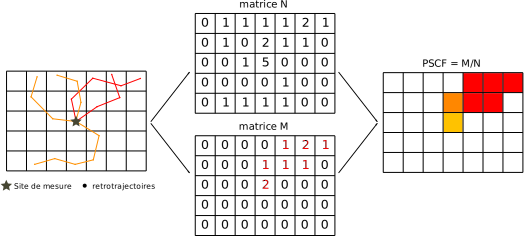
\includegraphics[width=0.9\linewidth]{chapter03/PSCF_method.pdf}
    \caption{Illustration de la méthode PSCF : les rétrotrajectoires depuis le site de
        mesure sont calculées, celles associées à une concentration seuil sont
        représentées en rouge, les autres en orange. Les matrices N et M s'obtiennent par
        simple décompte du nombre de rétrotrajectoires passées dans chaque cellule de
        taille prédéfinies, puis le ratio nous donne une estimation de l'origine
    géographique, représentée ici en terme d'intensité de rouge.}%
    \label{fig:chapter02/PSCF_method}
\end{figure}

\subsubsection{Application de la PSCF}%
\label{ssub:application_de_la_pscf}

\begin{tcolorbox}[colback=red!5!white,colframe=Melon,title=Note]
Cette partie synthétise dans un premier temps les résultats de~\cite{gollyOrganic2019},
dans lesquels mon implication a porté notamment sur le calcul et l'analyse PSCF, et dans
un second temps expose l'une des méthodes de validation possible des PMF grâce aux PSCF,
appliquée sur le site de l'OPE.
\end{tcolorbox}

\paragraph{Importance et origine géographique du MSA}%
\label{par:origine_terrestre_ou_marine_du_msa_}

Comme expliqué précedemment, une part importante des aérosols provient de sources
secondaires, c'est-à-dire du vieillissement et des réactions dans l'atmosphère. Une part
importante de ces aérosols secondaires est d'origine organique. Les travaux
de~\textcite{gollyOrganic2019}, s'attachent notamment à la quantification de cette matière
organique secondaire sur 5 sites ruraux en France pendant l'année 2013, par la mesure de
deux espèces issues de processus secondaires : le MSA et l'oxalate.  Nous avons pu montrer
que le MSA, considéré comme provenant de l'oxydation du DMS, peut contribuer jusqu'à 10 à
\SI{20}{\percent} de l'OC en période chaude, indiquant une forte proportion d'aérosols organiques
secondaires durant l'été. Mais surtout, le MSA est considéré comme provenant des émissions
de DMS du phytoplancton marin, au point qu'il est proposé comme méthode de séparation
entre le sulfate d'origine marine et ses autres provenances, en particulier en milieux
polaires.

En conduisant une analyse PSCF sur les \SI{25}{\percent} des jours les plus fortement chargés en MSA
sur les 5 sites, nous avons pu confirmer l'importance marine de ce composé. 
Cependant, une part non négligeable semble également provenir d'environnements
continentaux (voir
figure~\ref{fig:chapter03/golly_PSCF_MSA}), confortant les études suggérant des processus
d'émissions du MSA par des sources biologiques terrestres~\autocite{bozzettiArgon2017},
pouvant provenir des forêts ou des
sols~\autocite{jardineDimethyl2015,miyazakiSeasonal2012}.

L'une des implications directes de ces travaux résulte en l'ajout systématique du MSA
comme variable d'entrée des études PMF, quels que soient leurs localisations. En effet, le
signal du MSA est clairement distinct des autres espèces chimiques mesurées et représente
également une part important de la matière organique. Cette espèce est donc a minima
traceuse de processus secondaires présents sur l'ensemble de l'Europe occidentale.

\begin{figure}[ht!]
    \centering
    \includegraphics[width=0.9\linewidth]{chapter03/golly_PSCF_MSA.png}
    \caption{Probabilité de l'origine géographique du MSA, issue de l'article
        de~\textcite{gollyOrganic2019}. Bien que l'on retrouve l'origine marine du MSA,
        les sites de Dieulefit, OPE ou Peyrusse-Vieille indiquent également une forte
        probabilité d'origine terrestre de cette molécule.}%
    \label{fig:chapter03/golly_PSCF_MSA}
\end{figure}

\paragraph{Confrontation PSCF -- PMF}%
\label{par:confrontation_pscf_pmf}

Une autre utilisation de la PSCF consiste à croiser les informations issues de la PSCF et
des PMF.
En effet, il n'existe pas de moyen simple de valider le sens géochimique d'une solution
PMF autrement que l'expertise et les connaissances de l'utilisateur.

Pour estimer la fiabilité de la solution obtenue, il est possible de conduire une
étude PSCF sur les différents facteurs identifiés. On s'attend à ce que le
facteur \textit{sel de mer} provienne géographiquement d'un océan ou d'une mer par
exemple.

Un exemple d'utilisation de ce procédé est expliqué et illustré dans la section dédiée aux
PMF et couplées aux mesures isotopiques, section~\ref{sub:isotopie}.



\section{Incertitudes associées aux PMF}%
\label{sub:incertitudes_associées}

\begin{tcolorbox}[colback=red!5!white,colframe=Melon,title=Note]
    \todo{Mettre qqch ici}
\end{tcolorbox}

Le modèle PMF est maintenant relativement couramment utilisé dans le domaine de la
qualité de l'air. Seulement, peu d'études rapportent en même temps que leur solution
finale, les incertitudes associées. Or, le solveur ME-2 permet l'estimation de ces
incertitudes à travers les méthodes de bootstrap et de displacment (voir
section~\ref{par:incertitudes}).

Seulement, ces incertitudes ne sont rapportées par l'EPAPMF5.0 que pour les concentrations
des espèces chimiques des différents facteurs et non pour leurs contributions temporelles.
Notamment, lors de l'estimation de la variabilité via la technique du bootstrap, les différents facteurs
sont attribués aux facteurs de références d'après leur corrélation temporelle (par défaut
$r > 0.6$), mais seuls les profils chimiques sont rendus à l'utilisateur par la suite.
Une solution serait de manuellement explorer 100 solutions PMF, avec ou sans tirage
aléatoire des échantillons, pour estimer respectivement la variabilité provenant du modèle
statistique ou de la représentativité du jeu de donnée. Malheureusement, cette
répétabilité est beaucoup trop fastidieuse à faire à la main et ne peut pas s'automatiser à
partir de l'EPAPMF5.0. Or, il s'agit de l'implémentation du ME-2 la plus largement
utilisée. C'est pourtant un besoin important lors de la transférabilité de nos recherches
vers l'opérationnel, avec des questions très pratiques concernant l'incertitude
sur la contribution de telle source pour tels jours de pic de pollution en particulier.

Une ``astuce'' consiste alors à réestimer la variabilité des contributions temporelles
$X_{err}$ à partir de la variabilité de la composition chimique des profils, i.e. en gardant
$G$ fixe (celle de référence, $G_{ref}$) mais en utilisant les profils $F_{err}$ issus
des bootstraps et ambiguïté rotationelle :
\begin{align}
    \label{eq:hack_unc}
    X_{err} &= G_{ref} \times F_{err}.
\end{align}

Même si en théorie pour la méthode du bootstrap, à la fois $G$ et $F$ doivent
évoluer en même temps, cela donne une première estimation de la gamme d'incertitudes pour
chaque espèce et chaque jour d'observation.

Cette visualisation, présentée à titre d'exemple pour la PMF de Vif
figure~\ref{fig:chapter03/vif_nitraterich_all} permet de rapidement se rendre compte du
type d'incertitude prépondérant pour chacune des espèces chimiques (représentativité de
l'échantillonnage et ambiguïté rotationelle) mais également de la gamme de valeurs
possibles pour chaque jour étant donnée les incertitudes estimées.

\begin{figure}[ht]
    \centering
    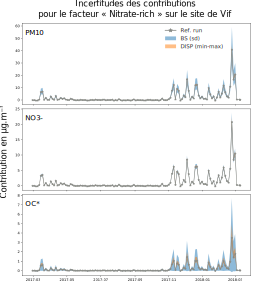
\includegraphics[width=0.8\linewidth]{chapter03/vif_nitraterich_all.pdf}
    \caption{Incertitudes temporelles des concentrations de \PMdix, \NOt{} et OC* dans le
        facteur Nitrate-rich de Vif (programme QAMECS/Mobil'air,
        \cite{borlazaFinescaleinprep.}) estimé par boostrap (écart type de 100 bootstraps en bleu)
        et displacment (min et max en orange). La solution de référence est représenté par les
    traits et étoiles grises.}%
    \label{fig:chapter03/vif_nitraterich_all}
\end{figure}


\section{Comparabilité des solutions}%
\label{sub:comparabilité_des_solutions}

Une problématique récurrente lors de l'utilisation des PMF est de se demander si les
profils que l'on obtient seraient nommés de la même façons par d'autres utilisateurs, et
si oui, comment peut-on évaluer la proximité géochimique de facteurs identiquement nommés
en différents endroits (spatiallement ou temporellement).

Les travaux de \cite{belisNew2015a} suggèrent l'utilisation conjointe de 2
métriques permettant d'estimer la distance géochimique entre 2 profils de facteurs.

\subsection{Méthodologie}%
\label{sub:méthodologie}

\paragraph{Distance de Pearson}%
\label{par:distance_de_pearson}

La distance de Pearson (\textit{Pearson distance} PD) estime la proximité entre 2 séries
de données en utilisant leur corrélation de Pearson, soit :
\begin{align}
    \label{eq:PD}
    PD &= 1 - r^2
\end{align}
avec $r$ la corrélation entre les 2 séries de données. Pour les profils chimiques des
facteurs, il s'agit de la concentration relative des espèces chimiques les constituants
(i.e. pourcentage massique de chacune des espèces).

Seulement, cette distance est très sensible aux extrêmes du fait de sa dépendance au
coefficient de correlation. Ainsi, si seul l'OC est similaire pour les 2 profils mais la
totalité des métaux présentent des concentrations très différentes, alors le PD pourra
être acceptable car l'OC présente des concentrations relatives bien supérieures à celles
des métaux (voir figure~\ref{fig:chapter03/PD_belis2015a}).
De plus, la distance de Pearson ne teste que l'hypothèse de relation linéaire entre les
deux profils, et non leur égalité stricte.

\begin{figure}[ht]
    \centering
    \includegraphics[width=1.0\linewidth]{chapter03/PD_belis2015a.png}
    \caption{Mesure de la distance de Pearson de 2 sources \textit{wood burning}. L'image
        de droite montre l'influence des espèces dominant la masse pour le calcul du PD, alors
        qu'en leur absence, le PD change drastiquement (image de droite). Source: adapté de
        \cite[figure 3]{belisNew2015}.
}%
    \label{fig:chapter03/PD_belis2015a}
\end{figure}


\paragraph{Distance identitaire standardisée}%
\label{par:distance_identitaire_standardisée}

Pour répondre aux problèmes soulevés par la distance de Pearson, \cite{belisNew2015}
proposent l'utilisation de la distance identitaire standardisée (\textit{Standardized
Identity Distance} SID). Sa formulation a légèrement évoluée entre son expression
initiale par~\cite{belisNew2015} et celle actuellement utilisée par
SPECIEUROPE\footnote{\url{https://source-apportionment.jrc.ec.europa.eu/Specieurope/index.aspx}}~\autocite{pernigottiSPECIEUROPE2016,pernigottiDeltaSA2018}.

L'idée principale consiste à exprimer la distance entre chaque paire d'espèces $i$ pour les 2
profils considérés $x$ et $y$ et la droite unitée, noté $ID_i$ pour \textit{identity
distance}, telle que:
\begin{align}
    \label{eq:IDi}
    ID_i &= \frac{1}{\sqrt{2}}|x_i - y_j|.
\end{align}
Aussi, afin de prendre en compte de manière homogène toutes les espèces et s'extraire du
biais sur-considérant les espèces prépondérantes à la masse, l'ID est normalisée par une
valeure proportionnelle à la moyenne de la masse de l'espèce $i$ dans le facteur $x$ et
$y$, appelée \textit{maximum acceptable distance} MAD, telle que:
\begin{align}
    \label{eq:MAD}
    MAD_i &= k \frac{1}{2}(x_i + y_i).
\end{align}
Ce procédé est illustré figure~\ref{fig:chapter03/SID_belis2015a}.

La SID est la moyenne de la somme des ratios entre l'ID et le MAD, telle que:
\begin{align}
    \label{eq:SIDi}
    SID &= \frac{1}{m}\sum_i^m\frac{ID_j}{MAD_j},
\end{align}
soit :
\begin{align}
    \label{eq:SID}
    SID &= \frac{\sqrt{2}}{km} \sum_i^m \frac{|x_i - y_i|}{x_i + y_i}.
\end{align}

\begin{figure}[ht]
    \centering
    \includegraphics[width=0.9\linewidth]{chapter03/SID_belis2015a.png}
    \caption{Illustration schématique de la distance SID. Légende originelle:
        Geometric representation of the identity distance (ID) as an indicator of
        similarity between two factor/source profiles. Left pane: $ID_{j,ab}$ between
        factor/sources $a$ and $b$ for species $j$ with acceptability thresholds (dotted lines);
        the dot represents point ($x_{ja}$, $y_{jb}$ ). Right pane: comparison of two
        hypothetical factor/sources with 10 common species.
        Source: \cite[figure 2]{belisNew2015}
}%
    \label{fig:chapter03/SID_belis2015a}
\end{figure}

\subsection{Implémentation et utilisation}%
\label{sub:implémentation_et_utilisation}

Ces 2 métriques de distances entre profils sont utiles pour l'aide à l'identification
d'un nouveau profils, notamment via SPECIEUROPE. Cependant, toutes les espèces chimiques
que nous utilisons ``en routine'' ne sont pas nécessairement présentes dans les profils de
SPECIEUROPE. Aussi, SPECIEUROPE nous permet essentiellement de comparer des profils déjà
existant dans cette base, et non
par exemple des PMF sur 2 sites non encore dans la base de donnée SPECIEUROPE.

\begin{tcolorbox}[colback=red!5!white,colframe=Melon,title=Note]
    Ainsi, pour comparer les profils chimiques issues d'une même méthodologie PMF (mêmes
    variables d'entrée, mêmes contraintes, etc) à différents lieux, j'ai ré-implémenté une version
    de deltaTool en python\footnote{Disponible dans le paquet
        \href{https://pypi.org/project/py4pm/}{py4pm}, dépot git:
        \url{https://gricad-gitlab.univ-grenoble-alpes.fr/webersa/py4pm}
    } permettant une
    utilisation plus flexible et une comparabilité des PMF étudiées pendant ma thèse.

    Le choix de $k$ de l'Eq.~\ref{eq:SID} pour le MAD a été porté à 1, similairement à
    \cite{pernigottiDeltaSA2018}, en absence d'information a priori sur la variabilité de ces
    profils.
\end{tcolorbox}

La question de la comparabilité des profils s'est posée majoritairement à 3 moments de ma
thèse :
\begin{enumerate}
    \item Comparer 15 PMF utilisant une méthodologie harmonisée en France (projet SOURCES);
    \item Étudier la variabilité fine échelle (i.e. à l'échelle d'une métropole) à travers
        3 sites de prélèvement dans un rayon de \SI{15}{\kilo\m} autour de Grenoble, France
        (projet Mobil'Air);
    \item Évaluer l'impact de l'ajout de traceurs organiques (acide pinique, phthalique,
        3-MBTCA et cellulose) par rapport à une PMF ``standard'' sur les 3 sites
        Grenoblois (projet Mobil'Air).
\end{enumerate}

Le premier item sera abondamment traité dans la section~\ref{sec:sources} de ce chapitre et
\textcite{weberComparison2019}, tandis que les 2 autres font l'objet d'un article en
cours de soumission par \textcite{borlazaFinescaleinprep.} et sont détaillés succinctement
dans la section~\ref{sub:processus_secondaires}.

\section{Amélioration des solutions PMF par ajout de traceurs spécifiques}%
\label{sec:amélioration_des_solutions_pmf}

\subsection{Apport de l'isotopie de l'azote sur la caractérisation des sources de pollution émettrices d’ammonium}%
\label{sub:isotopie}

\begin{tcolorbox}[colback=red!5!white,colframe=Melon,title=Note]
Les résultats présentés dans cette partie sont en partie issus d'un travail que j'ai
effectué antérieurement à ma
thèse dans l'équipe CHIANTI dans le cadre du projet INACS de l'ADEME portant sur
la caractérisation des épisodes de pollution printaniers au nitrate d'ammonium.
\end{tcolorbox}

\begin{tcolorbox}[colback=red!5!white,colframe=ProcessBlue,title=Note]
    Ces travaux ont été présentés dans le rapport INACS-2 (présenté en
    annexe~\ref{annexe:INACS}) et lors d'une présentation orale à l'EAC de Tours en 2016
    \autocite{weberNitrogen2016}.
    Un article est également en cours d'écriture sur ce sujet.  Les principales méthodes
    et résultats sont repris dans cette section.

    Certaines valeurs ne sont pas identiques entre le rapport INACS et celles présentées içi
    car ces travaux ont continué et certains paramètres ont changé entre la publication
    du rapport et l'écriture de la thèse.
\end{tcolorbox}


\subsubsection{Problématique}%
\label{ssub:problématique}

Dans de nombreuses PMF, il est rapporté un facteur secondaire inorganique contennant une
grande part du sulfate, du nitrate et de l'ammonium, indiquant la présence de sulfate
d'ammonium \ce{SO4(NH4)2} et nitrate d'ammonium \ce{NO3NH4}. Ces deux derniers facteurs sont
également souvent distincts, formant un facteur ``sulfate rich'', présentant le sulfate
d'ammonium mais sans nitrate, et ``nitrate rich'' présentant du nitrate d'ammonium mais
sans sulfate.

Le facteur \textit{Nitrate-rich} présente des émissions très saisonnières, responsables
des grands événements de dépassement des seuils d'alerte printanieris. Seulement,
s'agissant d'un facteur secondaire issu de réactions des \ce{NO_x} et de l'ammoniac
\ce{NH3} gazeux, sa provenance n'est pas clairement établie. En effet, si les \ce{NO_x}
sont supposés venir du traffic routier, la provenance de l'ammoniac peut aussi bien être
agricole via l'urée ou les fertilisants de synthèse que liée au trafic routier. Aussi, une
source importante contribuant pendant ces pics de pollution printaniers pourrait être la
combustion de biomasse domestique, notamment en vallées alpines, où cette source est
active et corrélée au nitrate d'ammonium au début du printemps.

\subsubsection{Objectifs et méthode}%
\label{ssub:objectif_et_methode}

L'isotopie donne potentiellement des informations importantes pour permettre l'estimation
des sources d'émission, seulement il n'est pas possible d'utiliser telles quelles dans une
analyse PMF et donc de traiter cette information pour identifier plus précisément la
source nitrate rich.  En effet, la PMF résoud une équation d'équilibre des masses et est
donc purement additive. Or, les mesures isotopiques se traduisent par une équation de
mélange, résultant en une moyenne pondérée de la signature isotopique des sources par
leurs contributions.

Par contre, s'il n'est pas possible d'inclure directement le signal isotopique dans les
PMF, il est possible d'effectuer un traitement en amont de la PMF, permettant de séparer
l'ammonium ou le nitrate en différentes ``sous espèces'', selon leurs sources de
provenances, grâce à l'isotopie.

Dans ce cadre, le programme INACS de l'ADEME a permis les mesures de l'isotopie de l'azote
du nitrate et de l'ammonium sur des cycles annuels complets pour 8 sites en France.
Parallèlement, les mesures de la signature isotopique à l'émission de différentes sources
ont été conduites, notamment en tunnel (émissions véhiculaires) et à l'émission de
cheminée (combustion de biomasse domestique), ainsi que de substances issues de sources
agricoles (fumier, fertilisant de synthèse, bâtiment d'élevage, etc).

Une partie du rapport établi suite à cette étude est disponible en annexe
\ref{annexe:INACS} et ne sont présentés ci-après que les étapes et les résultats majeurs.

\paragraph{Équation de mélange}%
\label{par:équation_de_mélange}

La première partie du programme INACS a montré que ces sources présentent des signatures
isotopiques de l'azote distinctes pour l'ammoniac, noté \dN(\NHq).
Nous pouvons alors, sous certaines conditions, proposer une déconvolution de l'équation de mélange
\begin{align}
    \dN(\NHq)_{atm} \cdot [NH_4^+]_{atm} &= \sum_{i=1}^{n} \dN(\NHq)_i \cdot [NH_4^+]_i
    \label{eq:melangeConcentration}
\end{align}
avec $[NH_4^+]_{atm} = \sum_{i=1}^n [NH_4^+]_i$ [\si{\ugm}] la concentration atmosphérique
d'ammonium résultant du mélange des $n$ sources.  L'équation~\ref{eq:melangeConcentration}
peut être réécrite en considérant $f_i = [NH_4^+]_i / [NH_4^+]_{atm}$~[-] comme étant la
contribution de la source $i$ au mélange final. Ainsi on a
\begin{align}
    \dN(\NHq)_{atm} &= \sum_{i=1}^n \dN(\NHq)_i \cdot f_i. 
    \label{eq:melangeContrib}
\end{align}

Selon certaines hypothèses, détaillées dans l'annexe~\ref{annexe:INACS}, en considérant
les trois sources précédemment citées supposées majoritaires, à savoir combustion de
biomasse, agricole et véhiculaire, et un coefficient de fractionnement \eN{} de
\num{-30}~‰
pour chaque observation de \dN(\NHq)$_{atm}$ le système
d'équation~\ref{eq:system1} suivant doit alors être vérifié :
\begin{numcases}{\label{eq:system1}}
    \small
    1 &$= f_{bio} + f_{agr} + f_{veh}$ \label{eq:bilanMass1} \\
    \dN(\NHt)_{atm} &$= f_{bio} \cdot \dN(\NHt)_{bio} + f_{agr} \cdot \dN(\NHt)_{agr} +
    f_{veh} \cdot \dN(\NHt)_{veh}$\label{eq:systemNH4}
    % \dN(\NHq)_{atm} &$= f_{bio} \cdot \dN(\NHq)_{bio} + f_{agr} \cdot \dN(\NHq)_{agr} + f_{veh} \cdot \dN(\NHq)_{veh}$ \label{eq:systemNH4}
\end{numcases}
où $f_{bio}$, $f_{agr}$ et $f_{veh}$ sont respectivement la contribution de la source de
biomasse, agricole et véhiculaire et $\dN(\NHt)_{bio}$, $\dN(\NHt)_{agr}$ et
$\dN(\NHt)_{veh}$ les compositions isotopiques respectives des sources biomasse, agricole
et véhiculaire.

\paragraph{Résolution par méthode Monte-Carlo}%
\label{par:résolution_par_méthode_monte_carlo}

La signature isotopique des sources étant connue avec une certainte incertitude, l'équation de
mélange est résolue par méthode Monte-Carlo : pour chaque jour d'observation, l'équation
\ref{eq:systemNH4} est résolue pour un triplet de valeurs possibles de chacune des
signatures isotopiques des 3 sources, suivant une loi normale établie par la moyenne et
l'écart type de chacun des prélèvements de ces sources. Le processus est répété 1000 fois
pour chaque jour d'observation, résultant ainsi en 1000 triplets $(f_{agr}, f_{bio},
f_{veh})$ possibles, permettant de calculer la concentration et l'incertitude associée de
l'ammonium apporté par chacune de ces sources.

\paragraph{Ajout d'une contrainte pour l'ammonium issu de la combustion de biomasse}%
\label{par:ajout_d_une_contrainte_pour_l_ammonium_issu_de_la_combustion_de_biomasse}

\subparagraph{Nécessité d'une nouvelle contrainte}%
\label{par:nécessité_d_une_nouvelle_contrainte}

Le système d'équation \ref{eq:system1} est sous-déterminée : il existe 3 inconnues pour
seulement 2 contraintes (bilan de masse et isotopie). De fortes incertitudes sont donc
attendues, voir des concentrations calculées qui seront invraisemblables, notamment pour les
concentrations de la combustion de biomasse.
Deux nouvelles contraintes pourraient être ajoutées pour ajouter de l'information et
réduire le degré de liberté du système : 1) une information sur l'isotopie de l'hydrogène
et 2) une connaissance \textit{a priori} de la géochimie des sources.  La deuxième
solution est retenue.  En effet un proxy de la combustion de biomasse, le lévoglucosan,
est déjà mesuré pour la quasi-totalité des sites d'études.

\subparagraph{Concentrations de lévoglucosan et d'ammonium}%
\label{par:concentrations_de_lévoglucosan_et_d_ammonium}

De par le recensement en une base de donnée unique de la filtrothèque de l'équipe
CHIANTI (voir \ref{sec:harmonisation_et_gestion_de_base_de_donnée}), il a été possible
d'estimer empiriquement des gammes de concentrations possibles pour l'ammonium en fonction
des concentrations en lévoglucosan. Puisque les vallées alpines sont connues pour présenter
des épisodes de pollutions aux particules fines dont la source est quasi exclusivement
la combustion de biomasse \autocite{piotAtmospheric2011,gollyEtude2014} et que le lévoglucosan
est considéré comme traceur univoque de la combustion de biomasse, en utilisant les
données chimiques de ces sites, il est possible de trouver une relation entre la
concentration de \NHq{} issue de la combustion de biomasse et la concentration en
lévoglucosan. 

Le seuil de concentration en lévoglucosan à \SI{5000}{\ngm} est considéré comme critère de
sélection des jours où la source biomasse est prépondérante. 
Pour ces jours-ci, le \NHq{} émis est considéré comme provenant de la combustion de
biomasse.
Avec ces hypothèses, une régression linéaire entre l'ammonium et le lévoglucosan montre la
relation $[\NHq] = 0.221 \times \text{[levoglucosan]}$ (trait plein sur la
figure~\ref{fig:correlNH4Levo}).
L'écart-type est volontairement choisi très large pour rendre compte du faible nombre
d'échantillons (18) et du caractère expérimental de cette relation (trait pointillés sur la
figure~\ref{fig:correlNH4Levo}).

Ainsi, l'équation suivante est ajoutée au système à résoudre
\begin{numcases}{\label{eq:system3}}
    f_{bio} &$= \{\mathcal{N}(m_{bio},\sigma_{bio})\}$ / [\NHq$_{total}$] \label{eq:bioChimie}\\
    1 &$= f_{bio} + f_{agr} + f_{veh}$ \label{eq:bilanMasse}\\
    \dN(\NHt)_{atm} &$= f_{bio} \cdot \dN(\NHt)_{bio} + f_{agr} \cdot \dN(\NHt)_{agr} + f_{veh} \cdot \dN(\NHt)_{veh}$\label{eq:isotopie}.
\end{numcases}
L'équation~\ref{eq:bioChimie} est une contrainte a priori et non isotopique. 
Elle réduit la liste des valeurs théoriquement possibles, tandis que
l'équation~\ref{eq:isotopie} sélectionne celles qui sont en accords avec l'observation
isotopique.

\begin{figure}[ht]
    \centering
    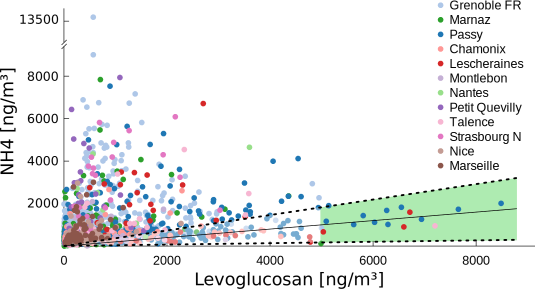
\includegraphics[width=0.7\textwidth]{figures/INACS/MCA_correlNH4Levo_alea.pdf}
    \caption{Estimation du ratio \NHq/lévoglucosan pour les jours de fortes concentrations en
        lévoglucosan. La droite noire en trait plein représente la droite $[\NHq_{bio}]=
        0.221 \times \text{[lévoglucosan]}$, les droites en trait pointillés les
        écart-types considérés ($\frac{1}{8}\times \text{[lévoglucosan]}$) et la zone
        verte les jours où la source de combustion de biomasse est considérée comme
        prépondérante ([lévoglucosan] > \SI{5000}{\ngm}]).
    }
    \label{fig:correlNH4Levo}
\end{figure}

\subsubsection{Détermination des sources de \NHq}%
\label{ssub:determination_des_sources_de_NHq}

\paragraph{Importance de la source agricole pour le \NHq}%
\label{par:importance_de_la_source_agricole_pour_le_nhq}

Le site rural de l'OPE est un site typique des tendances générales de l'ensemble des sites
d'études pour ces épisodes de fortes concentrations de PM printaniers.
Il est donc utilisé comme illustration dans la suite, pour des prélèvements s'étalant sur
l'année 2013.

Durant la période chaude (de mai à septembre) le fond atmosphérique en ammonium est très
majoritairement dû au secteur véhiculaire qui explique à lui seul \SI{90(8)}{\percent} du
\NHq{} total (\textit{cf.} figure~\ref{fig:timeSerieOPE}.a).
La quantité d'ammonium apportée par cette source est sensiblement constante autour
\SI{0.6(4)}{\ugm} tout au long de l'année (figure~\ref{fig:timeSerieOPE}.b).

D'après le modèle, les épisodes de printemps (mars et avril) sont imputables
majoritairement à la source agricole, qui apporte de l'ordre de \SI{80(10)}{\percent} du
\NHq{} ces jours-ci.  Ce secteur apporte jusqu'à \SI{5}{\ugm} d'ammonium le 2 avril, soit
plus de 8 fois l'apport moyen du véhiculaire.

\begin{figure}[ht]
    \centering
    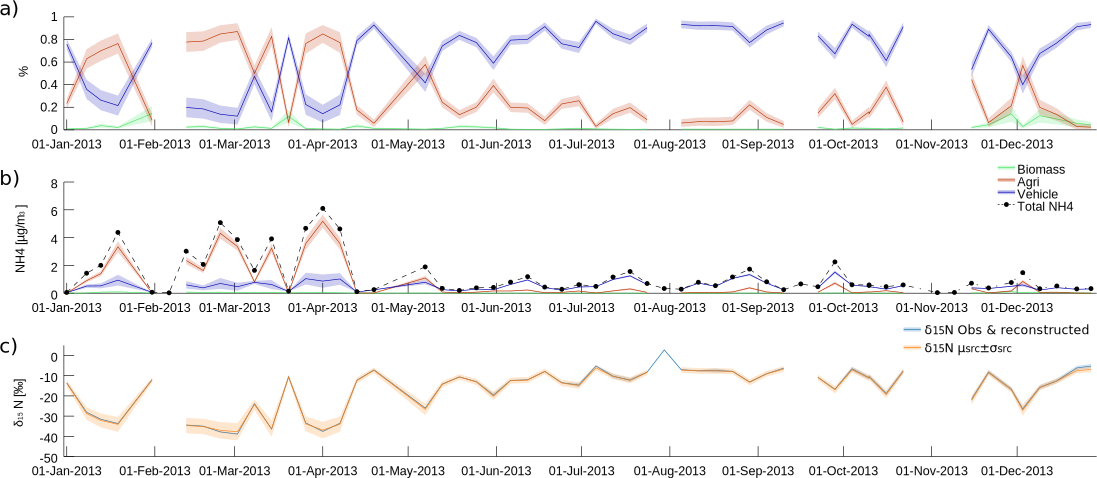
\includegraphics[width=1.0\linewidth]{figures/INACS/MCA_OPE_S3-BioFerVeh_e-30_timeSerie2013.pdf}
    \caption{Série temporelle du site de l'OPE. Sont représentés la moyenne de la densité
        de probabilité et l'écart-type (1$\sigma$) associé. \textbf{a)} Contribution
        relative de chaque source à l'observation. \textbf{b)} Contribution absolue de
        chaque source. Le trait noir pointillé est le \NHq{} observé. \textbf{c)}
        \dN{} observé et reconstruit en bleu, \dN{} reconstruit à partir de la totalité des
        valeurs des sources possibles en oranges.
    }
    \label{fig:timeSerieOPE}
\end{figure}

\paragraph{Fond atmosphérique de l'ensemble des sites} 

L'été, lorsque seule la source véhiculaire est active, la même quantité d'ammonium est
observée sur l'ensemble des sites considérés dans cette étude comme le montre la
figure~\ref{fig:summerNH4}.  La source véhiculaire est donc sensiblement constante sur
l'ensemble du territoire à raison de $\sim0.6$~\si{\ugm}.  Toutefois les sites de Lens et
de Turin semblent être au-dessus de ces tendances, et sont discutés en annexe
\ref{annexe:INACS}.

\paragraph{Épisodes synchrones à l'échelle du territoire}

Sur les sites étudiés, il apparait également que les pics de pollution sont synchrones à
l'échelle nationale : février 2012, février 2013 et mars 2013.  La plupart des pics de
pollution lors de ces événements sont attribués pour une grande part au secteur agricole.
La contribution du \NHq$_{agr}$ au \NHq{} total lors de ces épisodes est reportée sur la
figure~\ref{fig:contribSpringAgr}.

Les sites où l'influence du facteur agricole est la plus marquée sont les deux sites
ruraux de Revin et l'OPE pour lesquels les jours les plus impactés sont attribués à plus
de \SI{80}{\percent} à l'agriculture pour des concentrations excédent respectivement 7 et 5
\si{\ugm}, soit environ 10 fois plus que le fond atmosphérique.

\begin{figure}[ht]
    \begin{subfigure}[t]{0.5\textwidth}
    \begin{center}
    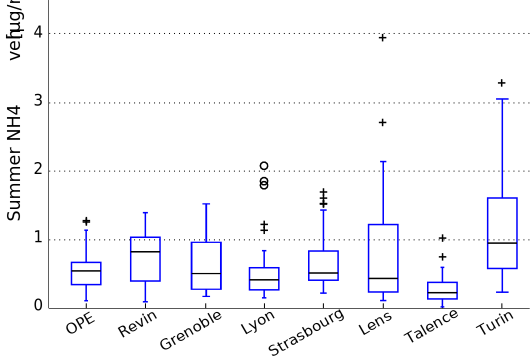
\includegraphics[width=.9\textwidth]{figures/INACS/MCA_contribSummerVeh.pdf}
    \end{center}
    \caption{Contribution moyenne de la source véhiculaire durant les jours de la période chaude.}
    \label{fig:summerNH4}
    \end{subfigure}
    \begin{subfigure}[t]{0.5\textwidth}
    \begin{center}
    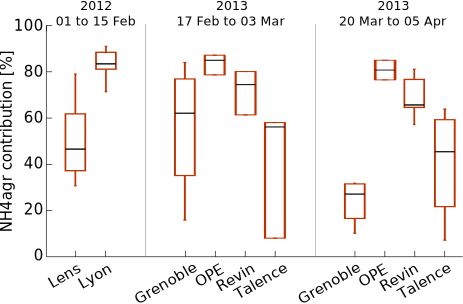
\includegraphics[width=.9\textwidth]{figures/INACS/MCA_contribSpringEventAgr.pdf}
    \end{center}
    \caption{Contribution relative moyenne de la source agricole pour les jours des trois
    pics de pollution printaniers observés.}
    \label{fig:contribSpringAgr}
    \end{subfigure}
    \caption{Contributions des sources véhiculaire et agricole.}
\end{figure}

\subsubsection{Utilisation couplée de l'isotopie et des PMF}%
\label{ssub:utilisation_couplée_de_l_isotopie_et_des_pmf}

\paragraph{Paramètrage de la PMF et solution de référence}%
\label{par:paramètrage_de_la_pmf_et_solution_de_référence}

Une fois le \NHq{} séparé en trois variables distinctes cette information peut être utilisée
dans une approche de type Positive Matrix Factorization (PMF) pour mieux comprendre la
dynamique des différents facteurs.
L'avantage majeur de l'utilisation de la PMF sera aussi de faire le lien entre les sources
du nitrate d'ammonium et les sources de PM.

Le site de l'OPE a été choisi pour tester la méthodologie car une étude PMF intégrant
les données chimiques de 2012 à 2014 pour la fraction \PMdc{} a déjà été conduite sur ce
site, offrant un comparatif intéressant pour le couplage isotopie/PMF.

Les variables utilisées sont donc les mêmes que celles de l'étude précédente
de~\cite{gollyCaracterisation2015} auxquelles s'ajoute le chlore. Elles sont rappelées dans le
tableau~\ref{tab:varPMF}.
Pour l'étude couplée chimie et isotopie, seul diffère le \NHq{} qui est séparé en trois
espèces \NHq$_{bio}$, \NHq$_{agr}$ et \NHq$_{veh}$. 

\begin{table}[ht]
    \centering
    \footnotesize
    \begin{tabular}{r P{2cm} P{1.5cm} P{5.0cm} P{3.0cm}}
        \toprule
                    & Matière carbonée       &   Métaux      &   Ions                                                &   Composés organiques \\
        \midrule
        PMF         & OC, EC                  & As, Pb, Ti, V & MSA, \NOt, \SOq, Oxalate, \ce{K+}, \ce{Na+}, \ce{Cl-}, \ce{Ca^2+}, \ce{Mg^2+}, \NHq   & Lévoglucosan, $\sum$polyols, HAP \\
        \midrule
        PMF + MC    & OC, EC                  & As, Pb, Ti, V & MSA, \NOt, \SOq, Oxalate, \ce{K+}, \ce{Na+}, \ce{Cl-}, \ce{Ca^2+}, \ce{Mg^2+}, \NHq$_{bio}$, \NHq$_{agr}$, \NHq$_{veh}$ & Levoglucosan, $\sum$polyols, HAP \\
        \midrule
        Incertitudes& Élargie (\SI{10}{\percent}, \SI{15}{\percent})  & \multicolumn{3}{P{10cm}}{Méthode proposée par \cite{gianiniSource2013}, sauf pour les trois \NHq$_{src}$ où $\sigma_{src}/4$ est utilisé.}\\
        \bottomrule
    \end{tabular}
    \caption{Espèces chimiques sélectionnées comme variables d'entrée dans les PMF pour la
    fraction \PMdc.}
    \label{tab:varPMF}
\end{table}

\paragraph{Solution obtenue}%
\label{par:solution_obtenue}

En substituant le \NHq{} par ses trois contributions \NHq$_{src}$ dans la PMF, il n'y a pas
de changement significatif pour les facteurs ne présentant pas déjà du \NHq (Secondaire
organique, Sels de mer, Sels de mer vieilli, Biogénique marin et Poussières/Biogénique
primaire).

Le \NHq$_{bio}$ se retrouve bien dans le facteur de combustion de biomasse à raison de
\SI{70}{\percent} du \NHq$_{bio}$ total.
Ce résultat était attendu car par construction le modèle Monte-Carlo introduit une
dépendance forte entre le lévoglucosan et le \NHq$_{bio}$.
Il est également intéressant de voir que \textit{seul} l'ammonium issu de la combustion
de biomasse se retrouve dans ce facteur.
Il faut cependant noter que le \NHq$_{bio}$ n'est pas entièrement attribué à ce facteur
mais également au facteur ``Nitrate rich'' (\SI{20}{\percent}) et dans une moindre mesure au sel
de mer vieilli (\SI{10}{\percent}).

La source Industrie/traffic se voit attribuer \SI{45}{\percent} de l'ammonium dit véhiculaire.
De plus, aucune des deux autres sources d'ammonium n'est présente dans ce facteur, ce qui
tend à accentuer l'étiquette ``traffic'' de ce facteur.
Une autre observation importante concerne l'activité de cette source au long de l'année :
l'industrie et le trafic sont connus pour avoir une activité constante, ou du moins non
saisonnière.
Or en n'utilisant pas les données isotopiques deux pics étaient observés fin février et
fin mars.
L'utilisation de l'isotopie diminue l'importance de ces pics, qui étaient
vraisemblablement une erreur d'attribution du \NHq{} entre le \NHq$_{veh}$ et le
\NHq$_{agr}$.

Une part non négligeable de l'ammonium dit véhiculaire est également retrouvée dans le
facteur Secondaire organique (\SI{>20}{\percent}).
Il serait intéressant d'investiguer plus en avant cet ammonium afin de savoir s'il s'agit
véritablement d'ammonium véhiculaire.

Enfin, le résultat sans doute le plus important réside dans l'identification du facteur
``Nitrate rich'', où la quasi-intégralité (\SI{>90}{\percent}) de l'ammonium agricole se retrouve.
Or il n'existe pas à notre connaissance une autre source ayant une signature isotopique
voisine ou plus négative en \dN{} que la source agricole.
Ainsi, il n'y a pas d'ambiguïté de source possible et le facteur ``Nitrate rich''
peut être identifié et renommé Agriculture.

\begin{figure}[ht]
    \centering
    \includegraphics[width=\textwidth]{INACS/PMF_OPE_contrib_profiles.pdf}
    \caption{
        Profils PMF pour une solution à 8 facteurs. Les histogrammes représentent la
        contribution de l'espèce dans chaque facteur par rapport à la masse de l'espèce
        totale et les courbes la contribution temporelle du facteur aux \PMdc{} [\si{\ugm}].
    }
    \label{fig:PMF}
\end{figure}

\paragraph{L'isotopie est-elle respectée ?}%
\label{par:l_isotopie_est_elle_respectée_}

Finalement, il est important de vérifier que la valeur isotopique reconstruite par les
concentrations de \NHq{} estimées par la PMF sont proches des valeurs estimées par méthode
Monte-Carlo.

Si les concentrations estimées par la PMF sont proches du modèle Monte-Carlo en été, on
observe cependant une erreur plus importante durant les pics de pollution (voir
figure~\ref{fig:PMFreconstruct}.a).
La conséquence est une reconstruction de l'isotopie moins bonne pendant ces périodes
(figure~\ref{fig:PMFreconstruct}.c).
Plus important encore, les prédictions de la PMF sont en dehors des écart-types du modèle
Monte-Carlo pour les pics de pollutions de fin février et fin mars-début avril, alors même
que la quantité totale d'ammonium est respectée (figure~\ref{fig:PMFreconstruct}.b).

Il est donc important de noter que les résultats de la PMF couplée vont dans le sens d'une
meilleure attribution des sources mais possèdent néanmoins encore une marge d'évolution
importante.
En ``forçant'' davantage la PMF d'après les données issues de Monte-Carlo,
l'importance du facteur agricole augmenterait et celle du trafic/industrie diminuerait.
L'estimation PMF présentée ici est donc une estimation basse de l'importance du facteur
agricole.

\begin{figure}[ht]
    \centering
    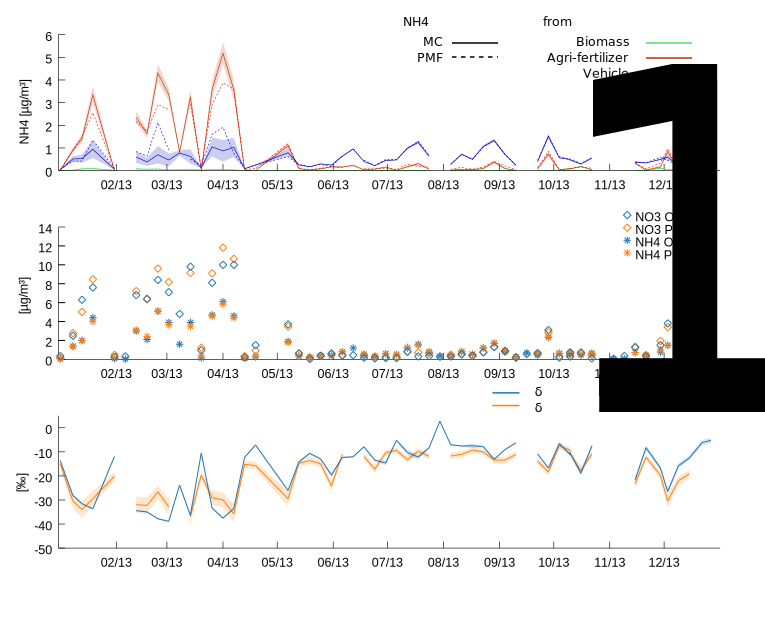
\includegraphics[width=1.0\textwidth]{figures/INACS/PMF_OPE_reconstruction.pdf}
    \caption{Reconstruction des variables \textbf{a)} \NHq$_{src}$, \textbf{b)} \NOt~et
        \NHq$_{tot}$ et \textbf{c)} \dN{} par modèle inverse d'après les données de sorties
        de PMF.
        \textbf{b)} Le \NOt{} prédit est celui reconstruit par la PMF et le \NHq{} est la
        somme des trois \NHq$_{src}$ donnés par la PMF.
        \textbf{c)} L'observation isotopique \dN{} est notée en trait plein bleu et le
        \dN{} reconstruit depuis les \NHq{} estimés par PMF en orange avec une incertitude
        correspondant à l'écart type de 2000 tirages aléatoires des valeurs des sources.
    }
    \label{fig:PMFreconstruct}
\end{figure}

\subsubsection{Conclusion}%
\label{ssub:conclusion_isotopie}


Grâce à l'isotopie, nous avons pu montrer que l'ammonium provient très majoritairement
de la source agricole lors des pics de pollutions printaniers, et ce à très grande échelle
spatiale, alors que la source véhiculaire semble bien constituer le fond ambiant en
nitrate d'ammonium tout le long de l'année.

Également, la méthodologie établie permet l'utilisation d'informations isotopiques dans
une étude PMF alors même que l'isotopie n'est pas additive, à condition d'effectuer un
traitement préalable du signal isotopique. Une contrainte forte de cette méthode est la
connaissance préalable de la signature isotopique des sources, ce qui rend la PMF moins
``agnostique'' sur la géochimie des facteurs.

Ainsi, la contribution du secteur agricole du facteur ``Nitrate rich'', déterminé dans de
nombreuseis PMF, est maintenant démontrée sur le site de l'OPE.
L'ajout de l'information isotopique permet également d'affiner la contribution et les
profils chimiques des autres facteurs contenant de l'ammonium, les rendant plus proches de
ce que l'on s'attend à observer (contribution du trafic homogène sur l'année, etc).

Cependant, l'une des limitations majeures concerne le choix des sources d'ammonium
considérées. Cette limitation est davantage explorée dans l'annexe~\ref{annexe:INACS}.

\subsection{Émission biogénique primaire}%
\label{sub:émission_biogénique_primaire}

\subsubsection{Problématique : la matière organique}%
\label{ssub:problématique_la_matière_organique}

La matière organique présente une large part d'espèces non identifiées et peut avoir de
nombreuses provenances. Bien que différentes espèces chimiques nous
permettent d'identifier et quantifier la contribution de différentes sources à la matière
organique (lévoglucosan et potatium pour la combustion de biomasse par exemple), certaines
espèces organiques mesurées ne présentent pas de corrélation évidente avec les facteurs
PMF usuel. C'est notamment le cas de l'arabitol et mannitol, molécules dont on sait
qu'elles sont fortement émises par les champignons et bactéries.
D'une façon générale, ces différentes sources biogéniques primaires, dont on sait qu'elles
existent mais dont les flux vers l'atmosphère sont très mal contraints, sont très souvent
``oubliées'' par les études de contribution des sources, soit par CTM soit par PMF.

Ainsi, mieux quantifier et identifier la provenance des sources d'émissions biogéniques
primaires permettrait peut-être d'identifier l'une des raisons de la sous-estimation des
PM (et particulièrement la composante carbonnée) par les modèles CTM, en pointant une source actuellement mal prise en compte dans ces
modèles.
De plus, nous avons pu montrer \parencite{samakeUnexpected2017} que la fraction biologique des
PM apportée par cette source liée aux bactéries et champignons pouvait avoir une certaine
importance sur le PO des PM, et il est donc important de la prendre en compte
correctement pour la suite de notre travail.

\begin{tcolorbox}[colback=red!5!white,colframe=Melon,title=Note]
    Cette étude a été menée dans le cadre de la thèse de~\cite{samakeAtmospheric2019}, et
    mon implication dans ces travaux concerne la partie recensement des données à partir
    de la base de donnée établie et présentée
    section~\ref{sec:harmonisation_et_gestion_de_base_de_donnée}, ainsi que l'utilisation
    et le traitement des résultats issues des PMF des projets DECOMBIO et SOURCES
    (travaux présentés en détail section~\ref{sec:sources}).
    Ils ont notamment conduit aux publications de
    \cite{samakeArabitol2019,samakePolyols2019,samakeHigh2020}, pour lesquels je suis
    co-auteur.
\end{tcolorbox}

\subsubsection{Synthèse grande échelle de la climatologie des polyols}%
\label{ssub:synthèse_grande_échelle_de_la_climatologie_des_polyols}

Pour comprendre la dynamique spatiale et temporelle des émissions biogéniques primaires,
les résultats de mesures de PM sur 28 sites Français présentant a minima un cycle annuel
de prélèvement analysant l'arabitol, le sorbitol, le mannitol et le glucose ont été
selectionnés~\autocite{samakePolyols2019}.

Nous avons montré que l'arabitol et le mannitol présentent de très fortes corrélations 
($0.58 \leq r^2 \leq 0.93$), avec un coefficient de droite de régression entre 0.59 et
1.10 pour un intercepe faible (toujours inférieur à \SI{9}{\ngm}). Ainsi, il parait
raisonnable de penser que ces 2 espèces sont co-émises par une ou plusieurs sources.
Le sorbitol et le glucose présentent quant à eux des dynamiques propres, non
nécessairement corrélées à l'arabitol ou au mannitol.
L'arabitol et le mannitol sont sommés et appelés \textit{polyols} par la suite.

Les polyols, en plus d'être ubiquitaires, présentent le même signal saisonnier sur l'ensemble
des sites d'études (voir figure~\ref{fig:polyols_samake2019}) et sont davantage présents
dans la fraction grossière (\PMdix) que fine (\PMdc), avec des concentrations variant de 
\SI{7.5\pm10.9}{\ngm} à \SI{27.8\pm33.3}{\ngm} pour les \PMdc, et
\SI{48.9\pm38.2}{\ngm} à \SI{73.5\pm61.8}{\ngm} pour les \PMdix, sur respectivement le site de
Revin et de l'OPE, correspondant à un ratio \PMdix/\PMdc{} variant en moyenne de 3 à 5.
Cette ségrégation suivant la taille des particules est identique pour le glucose.

Les polyols ne représentent cependant qu'une faible fraction de la matière organique. En
effet, en considérant un ratio entre l'OM et l'OC de 1.8 typique des écosystèmes d'Europe
de l'ouest, les polyols ne représentent qu'entre \SIrange{0.1}{2.1}{\percent} de l'OM. La
même contribution relative est trouvée pour le glucose.

\begin{figure}[ht]
    \centering
    \includegraphics[width=1\linewidth]{chapter03/polyols_samake2019.png}
    \caption{
        Distribution spatio-temporelle des concentrations de polyols (moyenne et écart
        type) en \si{\ngm}.
        Chaque saison est représentée par au moins 20 points de mesure.
        Source : \cite[figure 6]{samakePolyols2019}.
    }%
    \label{fig:polyols_samake2019}
\end{figure}

La taille des spores ou enveloppes microbiennes riches en polyols, généralement supra
micrométrique (typiquement de \SI{2}{\micro\m} à \SI{10}{\micro\m}), ainsi que l'activité
biologique importante en été et très ralentie en hiver viennent grandement conforter
l'hypothèse biogénique de ces composés.

Cette hypothèse a été testée par \cite{samakeArabitol2019} sur le site de
l'OPE, où la cellulose a été mesurée sur 2 années de prélèvements et les différentes
activités agricoles avoisinantes enregistrées (voir
figure~\ref{fig:ope_polyols_cellullose_agri}).
La coïncidence entre l'augmentation des concentrations des polyols, de la cellulose
(traceuse des débris de plantes) et des moissons, mais une bien plus faible concomitance
avec les labours, confortent encore une fois la provenance biogénique, mais précisent cette
fois le compartiment en question : les polyols proviennent très certainement des plantes
et non du sol.

Pour s'en assurer, une troisième étude, analysant l'ADN de prélèvement d'échantillon
de plantes, de sols et d'aérosols du site l'OPE, \autocite{samakeHigh2020} précise que
l'ADN retrouvée dans les aérosols correspond bien à des taxons de bactéries et champignons
originaires de la strate herbacée et non du sol.

\begin{figure}[ht]
    \centering
    \includegraphics[width=1.0\linewidth]{chapter03/ope_polyols_cellulose_agri_samake2019.png}
    \caption{
        Évolution conjointe des concentrations de polyols, cellulose, glucose et des
        activités agricoles sur le site de l'OPE de 2012 à 2018.
        Les activités de 69 parcelles environnants le site de prélèvement sont
        comptabilisées et agrégées en période de 12 jours.
        Après 2014, seuls les enregistrements pour 2 parcelles étaient disponibles, les
        valeurs sont donc multipliées arbitrairement par 10 pour cette période.
        Source : \cite[figure 6]{samakeArabitol2019}.
    }%
    \label{fig:ope_polyols_cellullose_agri}
\end{figure}

\subsubsection{Contribution des émissions biogéniques primaires aux \PMdix}%
\label{ssub:contribution_des_émissions_biogéniques_primaires_aux_pmdix}

Maintenant que l'origine biogénique des polyols est acquise, il reste à quantifier
l'importance de cette source biogénique primaire à l'ensemble des PM.
Puisque les polyols tracent de manière non équivoque cette source, l'ajout de ces espèces dans
les PMF permet d'identifier un profil biogénique primaire.

Pour ce faire, les 16 PMF issues du programme DECOMBIO et SOURCES ont utilisées les polyols
dans le jeu d'espèces sélectionné. Sur ces PMF, un facteur \textit{Primary biogenic
organic aerosol} ou PBOA a systématiquement été identifié, comprenant la quasi-totalité
des polyols.

La contribution de ce facteur à la matière organique totale varie de \SI{6}{\percent} à \SI{28}{\percent}, pour une
moyenne et écart-type de \SI{13\pm6}{\percent} en moyenne annuelle, mais peut représenter
plus de \SI{40}{\percent} de la matière organique en moyenne estivale à certains sites (voir
figure~\ref{fig:chapter03/pboa_pmf_samake2019}).
De fait, cette source d'émission représente un secteur d'émission important pour comprendre
les concentrations ambiantes de PM organiques, notamment en période chaude.

On peut se demander si ce facteur est entièrement d'origine primaire et n'agrège pas une
partie d'aérosol organique biogénique secondaire. En l'absence d'espèce tracant les
processus secondaires (comme le 3-MBTCA ou l'acide pinic), cette possibilité reste
ouverte.  Cette hypothèse parait cependant peu probable. En effet, le ratio OC/polyols du
profil PBOA est relativement peu variable entre les sites, alors qu'il serait peu
probable que la variabilité des processus secondaires conduisent à une concentration d'OC
identique sur l'ensemble de ces sites.  Aussi, les ratios OC/polyols des profils PBOA
(autour de 16) sont bien dans la gamme attendue de variabilité des spores de champignons
(entre 12 et 27), d'après \cite{bauerSignificant2008,yttriSource2011}.

\begin{figure}[ht]
    \centering
    \includegraphics[width=0.7\linewidth]{chapter03/pboa_pmf_samake2019.png}
    \caption{
        Mass contribution of polyols to OM in the PBOA factor, and relative contributions
        of the OM PBOA factor to the total OM in PM for the 16 studied sites where the
        PMF model was run, over the year and summertime only. Stars and circles refer to
        urban sites without and with Alpine valley influence, respectively. Pentagons
        correspond to traffic sites and diamonds to rural sites.
        Source : \cite[figure 9]{samakePolyols2019}.
    }%
    \label{fig:chapter03/pboa_pmf_samake2019}
\end{figure}

\subsubsection{Conclusion}%
\label{ssub:conclusion_polyols}

Nous avons donc montré que les polyols (arabitol et mannitol) sont des traceurs de
l'activité biologiques, notamment de la strate herbacée. Leur présence est ubiquitaire
mais représente seulement 0.1 à \SI{2.1}{\percent} de la matière organique des \PMdix.

Ainsi, ces études approfondies sur la dynamique et la provenance des polyols nous ont
permis de les identifier comme étant des espèces traceuses de source unique et présentes
sur une large étendue spatiale. Leur ajout dans les études PMF nous permet donc
l'isolement d'une source biogénique primaire provenant de l'activité biologique fongique
et bactérienne.

Leur ajout dans les analyses multifactorielles nous apprend que la contribution de ce
facteur PBOA à la matière organique totale varie de façons importante selon la saison,
mais peut représenter jusqu'à \SI{40}{\percent} de la matière organique en moyenne
estivale sur certains sites étudiés, en faisant un facteur important pour comprendre la
dynamique des PM en période chaude.

Cependant, les polyols ne sont pas la seule source d'émission primaire biogénique : on
peut notamment penser aux débris végétaux par exemple, ce qui reste à étudier. De même,
la question de la part secondaire provenant d'oxydation des composés biogéniques présents
dans ce facteur reste ouverte, en l'absence d'espèce traceuse de processus secondaire
comme le 3-MBTCA ou l'acide pinique. La section suivante~\ref{sub:processus_secondaires}
permettra de répondre en partie à cette question.

\subsection{Variabilité fine échelle, processus secondaires et traceurs organiques}%
\label{sub:processus_secondaires}

Afin de tenter de répondre à la problématique de la contribution des facteurs secondaires
aux PM, 3 sites de prélèvement sur Grenoble et sa périphérie (fond urbain : Les frènes
(LF), hypercentre : Caserne de Bonne (CB) et périurbain : Vif (Vif)) ont été choisis pour
établir une étude PMF incluant de nouveaux traceurs organiques spécifiques des processus
d'oxydations secondaires : le 3-MBTCA, l'acide pinique et l'acide phtalique. Sur cette
étude, la cellulose a également été mesurée pour essayer de distinguer potentiellement
différentes émissions biogéniques.

Aussi, la proximité géographique des 3 sites --tous dans un rayon de \SI{15}{\kilo\m}--
permet l'estimation de la variabilité fine échelle de l'ensemble des sources identifiées
par la PMF.

\begin{tcolorbox}[colback=red!5!white,colframe=Melon,title=Note]
    Cette partie s'appuie sur les travaux de \cite{borlazaFinescaleinprep.}, dont je suis
    second auteur, lors du projet Mobil'Air/QAMECS, destiné également à évaluer l'impact
    sur la qualité de l'air d'une zone à faible émission dans la métropole grenobloise
    (\url{https://mobilair.univ-grenoble-alpes.fr/}).
    L'intégralité du papier est disponible en annexe~\ref{annexe:borlazaSA}.
\end{tcolorbox}

\subsubsection{Variabilités saisonières}%
\label{ssub:variabilites_saisonières}

La cellulose étant très rarement mesurée, ainsi que les acides organiques, nous
présentons içi dans un premier temps les mesures de concentrations obtenues sur l'année
2017-2018 pour les 3 sites, en comparaison avec d'autres espèces plus communément
mesurées.

\paragraph{Corrélation entre espèces}%
\label{par:correlation_entre_especes}

\subparagraph{Oxydation secondaire biogénique}%
\label{par:oxydation_secondaire_biogénique}

On s'aperçoit tout d'abord que le 3-MBTCA et l'acide pinique présentent de très fortes
corrélations sur les 3 sites, avec un cycle saisonnier fort et d'importantes concentrations
en été (voir figure~\ref{fig:borlaza_evolution_temporelle}). Du fait de l'activité
photochimique conduisant à la formation d'espèces secondaires issues des terpènes en
cette période, ce résultat était attendu. On observe aussi de grandes variations de
concentrations à faible échelle temporelle (de l'ordre de quelques jours). Ces espèces
sont en effet très réactives et présentent un temps de demie-vie court dans l'atmosphère.

Aussi, ces espèces partagent le cycle saisonnier du MSA, mais présentent cependant des
contributions asynchrones, indiquant donc des processus secondaires ou de transport
différenciés.

\subparagraph{Polyols et cellulose}%
\label{par:oxydation_secondaire_anthrophique}

Comme attendue d'après \cite{samakePolyols2019}, les polyols ont un cycle saisonier très
marqués avec une forte concentration en été et faible en hiver. Ce cycle est aussi
présent pour la cellulose, bien que cependant moins marqué. En revanche, la durée où de
la cellulose est présente dans l'atmosphère est beaucoup plus grande que pour les
polyols.  Ainsi, les sources émettrices de polyols et de cellulose ne peuvent pas être
entièrement les mêmes.

\subparagraph{Sulfate et acide phthalic}%
\label{par:sulfate_et_acide_phthalic}

L'acide phthalique est en très faible concentration tout le long de l'année d'étude,
exceptés quelques pics très restreints temporellement. La synchronicité de ces pics avec
de fortes concentrations en sulfate est également observée, mais n'est pas totalement
expliquée pour l'instant.
Une hypothèse pourrait être une production commune dans les brouillards, fréquents en
hiver dans la cuvette Grenobloise.


\begin{figure}[ht]
    \centering
    \includegraphics[width=1\linewidth]{chapter03/borlaza/AllInOne.pdf}
    \caption{
        Évolutions temporelles de \textbf{a)} l'acide phthalic, \textbf{b)} l'acide
        pinic, \textbf{c)} le 3-MBTCA, \textbf{d)} le MSA, \textbf{e)} les polyols
        (arabitol+mannitol), \textbf{f)} la cellulose, \textbf{g)} le sulfate et
        \textbf{h)} le cuivre pour les 3 sites du bassin grenoblois (LF en orange, CB en
        bleu et Vif en vert).
    }%
    \label{fig:borlaza_evolution_temporelle}
\end{figure}

\paragraph{Similitude et diversité inter-site}%
\label{par:similitude_et_diversité_inter_site}

Lorsque l'on compare entre elles les mesures réalisées sur les différents sites, de très
fortes corrélations sont observées pour les ions et espèces organiques, à l'exception
notoire de la cellulose, qui semble avoir une dynamique propre sur chacun des sites
(figure~\ref{fig:chapter03/borlaza/correlation}).

De même, une partie des espèces métalliques montre des variabilités fortes entre sites.
Les traceurs du trafic routier (Cu et Fe) semblent indiquer une proximité entre les sites
de LF et CB, alors que le site de Vif présente un signal différent. Il en est de même
pour les traceurs des poussières crustales (\ce{Ca^{2+}}, Al et Ti). Ces différences sont
discutées plus en avant dans l'article proposé en annexe~\ref{annexe:borlazaSA}.

\begin{figure}[ht]
    \centering
    \includegraphics[width=1\linewidth]{chapter03/borlaza/correlation.png}
    \caption{Corrélations de Pearson entre les concentrations temporelles des espèces
        mesurées entre les 3 paires de sites (LF-CB, LF-Vif et CB-Vif)}%
    \label{fig:chapter03/borlaza/correlation}
\end{figure}

\subsubsection{Résultats PMF}%
\label{ssub:résultats_pmf}

Afin d'estimer l'impacte de l'ajout de la cellulose, des acides pinique et phthalique et
du 3-MBTCA, une PMF ``classique'' (i.e. sans ces nouvelles espèces et telle que
réalisée dans le programme SOURCES) sert de référence, et une PMF ``organique'' incluant
ces espèces mais respectant strictement les autres paramètres de la PMF classique permet
l'évaluation de leurs effets.  Les PMF sont calculées indépendamment pour chacun des 3
sites.  10 facteurs sont identifiés sur les 3 sites pour la PMF classique, résumés dans
le tableau~\ref{tab:pmf_mobilair_species}.

\begin{table}[ht]
    \begin{ThreePartTable}
        \centering
        \caption{Résumé des facteurs PMF identifiés sur les 3 sites grâce à leurs traceurs
        spécifiques.}
        \footnotesize
        \label{tab:pmf_mobilair_species}
        \begin{tabular}{ll}
            \toprule
            Identified factors & Specific tracers\\
            \midrule
            Biomass burning              & Levoglucosan, mannosan, \ce{K+}, Rb, \ce{Cl-}\\
            Primary traffic              & EC, \ce{Ca^{2+}}, Cu, Fe, Sb, Sn\\
            Nitrate-rich                 & \ce{NO3-}, \ce{NH4+}, phthalic acid\\
            Sulfate-rich                 & \ce{SO4^{2-}}, \ce{NH4+}, Se, phthalic acid \\
            Mineral dust                 & \ce{Ca^{2+}}\tnote{*}, Al, Ti, V\\
            Sea/road salt                & \ce{Na+}, \ce{Cl-}\\
            Aged sea salt                & \ce{Na+}, \ce{Mg^{2+}} \\
            Industrial                   & As, Cd, Cr, Mn, Mo, Ni, Pb, Zn\\
            Primary biogenic             & Polyols, cellulose\\
            MSA-rich                     & MSA\\
            Secondary biogenic oxidation\tnote{a} & 3-MBTCA, pinic acid\\
            \bottomrule
        \end{tabular}
        \begin{tablenotes}
        \item[*] Le site de Vif ne présente pas \ce{Ca^{2+}} dans ce facteur.
        \item[a] Seulement identifié pour les PMF organiques.
        \end{tablenotes}
    \end{ThreePartTable}
\end{table}

\paragraph{Nouveau facteur d'oxydation secondaire biogénique}%
\label{par:nouveau_facteur_d_oxydation_secondaire_biogénique}

Lors de l'ajout des nouvelles espèces organiques, un nouveau facteur apparaît, riche en
3-MBTCA et acide pinique et dont la contribution est maximale en été (voir la composition
et contribution temporelle de ce profil sur le site de CB
figure~\ref{fig:chapter03/borlaza/CB-SBO}).  Ce facteur apporte jusqu'à \SI{10}{\ugm} de
\PMdix{} certains jours d'été, en faisant l'un des facteurs majeurs contribuant aux
\PMdix{} certains jours.  Aussi, une part importante de l'OC est amenée par ce facteur
(environ \SI{10}{\percent} de l'OC total en moyenne annuelle), mais également du sulfate (environ
\SI{15}{\percent}), suggérant la présence de composés organiques sulfatés.  Ainsi, en
moyenne estivale, c'est entre \SI{20}{\percent} et \SI{40}{\percent} de la matière
organique qui sont apportés par ce facteur selon le site considéré, ce qui en fait le
facteur principal d'apport de matière organique pendant cette période.

\paragraph{Primaire biogénique}%
\label{par:primaire_biogénique}

Le deuxième facteur présentant d'importantes contributions de ces traceurs organiques est
le profil d'émission primaire biogénique (voir
figure~\ref{fig:chapter03/borlaza/LF-PBOA}). Notamment, près de \SI{60}{\percent} de la
cellulose est apporté par ce facteur, renforcant l'hypothèse de l'émission de ce facteur
par la strate herbacée (comme expliqué en
section~\ref{sub:émission_biogénique_primaire}). Aussi, et comme suspecté auparavant, ce
facteur est également responsable d'environ \SI{20}{\percent} de l'acide pinique et du
3-MBTCA, et par conséquent une part (assez faible) de la matière organique ne semble pas
d'origine primaire mais bien secondaire. Il est à noter également que la quantité totale
de matière organique ou de \PMdix{} expliquée par ce facteur ne varie pas avec l'ajout de
ces nouveaux traceurs organiques (voir
figure~\ref{fig:chapter03/borlaza/comparaison-classique-orga}), et de manière générale, à
part l'arrivée d'une part de la cellulose et de l'acide pinique et 3-MBTCA, la composition chimique de
ce facteur reste identique entre la PMF de référence et la PMF ``organique''.

\begin{figure}[ht]
    \centering
    \begin{subfigure}[t]{1\textwidth}
    \begin{center}
        \includegraphics[width=1\linewidth]{chapter03/borlaza/CB-Secondary biogenic oxidation.pdf}
    \end{center}
    \caption{Composition chimique et contribution temporelle aux \PMdix{} du facteur
    d'oxydation biogénique secondaire sur le site d'hypercentre CB.}%
    \label{fig:chapter03/borlaza/CB-SBO}
    \end{subfigure}
    \begin{subfigure}[t]{1\textwidth}
    \begin{center}
        \includegraphics[width=1\linewidth]{chapter03/borlaza/LF-Primary biogenic.pdf}
    \end{center}
    \caption{Composition chimique et contribution temporelle aux \PMdix{} du facteur
    d'émission primaire biogénique sur le site de fond urbain LF.}%
    \label{fig:chapter03/borlaza/LF-PBOA}
    \end{subfigure}
    \caption{Profil chimique et contribution temporelle aux \PMdix{} des 2 facteurs
        majoritairement impactés par l'ajout de la cellulose, acide pinique et phthalique
        et 3-MBTCA.
    }%
    \label{fig:chapter03/borlaza/pmf_profiles}
\end{figure}

\begin{figure}[ht]
    \centering
    \includegraphics[width=1\linewidth]{chapter03/borlaza/Comparison_orga-woOrga_profile_Primary biogenic_LF.png}
    \caption{Comparaison du profil chimique du facteur primaire biogénique sur le site de
        fond urbain LF entre la PMF classique (en bleue) et celle incluant les nouvelles
    espèces organiques (en orange).}%
    \label{fig:chapter03/borlaza/comparaison-classique-orga}
\end{figure}

\paragraph{Contributions des facteurs aux \PMdix}%
\label{par:contributions_des_facteurs_aux_pmdix}

Comparé aux PMF classiques, la différence majeure de la contribution aux \PMdix{} réside
en la diminution de l'importance du facteur sulfate rich au profit du facteur représentant
l'oxydation biogénique secondaire (voir
figure~\ref{fig:chapter03/borlaza/Comparison_orga-woOrga_absolute}).  En effet, on
observe une baisse entre \SI{1}{\ugm} et \SI{2}{\ugm} de la contribution du facteur
sulfate rich en moyenne annuelle sur les 3 sites, et une contribution équivalente à la
baisse du suflate rich pour le nouveau facteur d'oxydation secondaire biogénique.

Ainsi, l'ajout des nouveaux traceurs organiques a permis de mieux séparer le facteur
sulfate rich, qui comportait une part importante de l'OC, en deux facteurs de typologie
plus claire : secondaire inorganique sulfaté (i.e. sulfate rich) et secondaire organique
biogénique.

\begin{figure}[ht]
    \centering
    \includegraphics[width=1\linewidth]{chapter03/borlaza/Comparison_orga-woOrga_absolute.pdf}
    \caption{Comparaison des contributions annuelles des différents facteurs aux \PMdix{}
    pour les 3 sites entre les PMF classiques et organiques.}%
    \label{fig:chapter03/borlaza/Comparison_orga-woOrga_absolute}
\end{figure}

\subsubsection{Conclusion}%
\label{ssub:conclusion_organique}

Ainsi, en plus des conclusions sur les sources de PM et la variabilité fine échelle, qui
sont abondamment discutés dans l'article et rapidement rappelée ici, cette étude
multi-sites sur le bassin de la métropole grenobloise nous permet les conclusions
suivantes :
\begin{itemize}
    \item La variabilité des sources de \PMdix{} à l'échelle d'une moyenne métropole est
        relativement faible et les sites de fond urbain sont suffisamment représentatifs
        de l'ensemble de la métropole.
    \item La cellulose semble présenter un cycle saisonnier, mais des variabilités
        importantes à cette échelle spatiale sont également observées, indiquant très
        certainement des sources très locales de ce composé.
    \item Les phénomènes d'oxydation secondaires de la matière organique émise par les
        phénomènes biologiques (terpènes…) peuvent être ``capturés'' par une PMF sur
        filtres, notamment grâce au 3-MBTCA et à l'acide pinique.
\end{itemize}

Méthodologiquement, l'ajout de nouveaux traceurs spécifiques permet, même sur une
solution à 10 facteurs, de mieux séparer certains facteurs. Notamment, le 3-MBTCA et
l'acide pinique permettent une meilleure estimation du facteur inorganique secondaire
\textit{Sulfate rich} qui était jusqu'alors un mélange entre de l'inorganique et de
l'organique.  Cependant, l'ajout de la cellulose, présentant des évolutions de
concentrations assez différenciées des celles des polyols, ne permet pas l'identification d'un nouveau facteur
dans la solution présentée ici. En revanche, lors de nos essais sur cette PMF, nous avons
expérimenté plusieurs incertitudes pour cette espèce, et un ``seuil'' aux alentours de
\SI{15}{\percent} d'incertitude fait basculer la solution de 11 à 12 facteurs,
faisant apparaître un nouveau facteur très incertain statistiquement, comportant la
majorité de la cellulose.

Aussi, et dans la suite de la discussion de la section précédente
\ref{ssub:synthèse_grande_échelle_de_la_climatologie_des_polyols}, l'identification d'un
facteur d'oxydation secondaire en été ne change pas la contribution du profil primaire
biogénique, ce qui indique que ce facteur est suffissament contraint et bien déterminé
par ces espèces chimiques.

\section{Résultats du programme SOURCES}%
\label{sec:sources}

\subsection{Introduction}

Les travaux présentés précédemment nous apprennent que les solutions d'une étude PMF sont
très dépendantes des variables utilisées. Ainsi, il est compliqué de comparer 2 PMF
réalisées avec des méthodologies différentes.

Le projet SOURCES avait pour ambition d'établir une synthèse nationale des
sources de PM, à travers des approches site-recepteurs --et donc PMF-- afin être au plus
près des observations de terrains.
Ainsi, 15 sites d'études ont été sélectionnés, reflétant une diversité d'environnements
urbains de France métropolitaine, pour établir une méthodologie harmonisée d'étude PMF
incluant :
\begin{itemize}
    \item Une estimation des incertitudes communes,
    \item Les mêmes espèces chimiques sélectionnées,
    \item Les mêmes contraintes appliquées au modèle,
    \item Une estimation des incertitudes sur les solutions obtenues,
\end{itemize}
et ainsi établir une phénoménologie des sources de PM à l'échelle nationale.
Le rapport établi grâce au post-doctorat de Dalia Salameh,
décrit en détail la méthodologie utilisée ainsi que les profils de sources et les
contributions temporelles obtenues \parencite{favezTraitement2017}.

Dans cette partie, seules sont discutées la comparaison géochimique des différents
facteurs ainsi que la variabilité de leurs incertitudes.

\begin{tcolorbox}[colback=red!5!white,colframe=Melon,title=Note]
    Le travail de recensement et d'établissement de cette méthodologie a été conduit lors
    du post-doctorat de Dalia Salameh, et a conduit à l'écriture du rapport 
    \cite{favezTraitement2017} (Français). Ce travail a été poursuivi durant ma thèse,
    notamment sur la partie concernant la comparabilité et variabilité des profils
    chimiques, et a été valorisé dans le papier \cite{weberComparison2019}, présenté ici.
    Le complément d'information est disponible sur \url{http://pmsource.u-ga.fr} et en
    annexe~\ref{annexe:SOURCES_SI}.
\end{tcolorbox}

\begin{tcolorbox}[colback=red!5!white,colframe=Melon,title=Note]
    Devant la quantité de donnée générée par cette étude, j'ai mis en ligne un site web,
    servant entre autres de complément d'information à l'article, mais aussi permettant aux
    utilisateurs d'explorer eux-mêmes l'entièreté des solutions obtenues (profils
    chimiques, contributions, incertitudes, deltaTool…) : \url{http://pmsource.u-ga.fr}.

    Au 20 juillet 2020, ce site a déjà été visionné par plus de 400 personnes provenant
    d'une vingtaine de pays, donc \SI{30}{\percent} y sont revenus plusieurs fois.
\end{tcolorbox}

\subsection{Comparison of PM\textsubscript{10} sources profiles at 15 french sites using a harmonized constrained positive matrix factorization approach}%
\label{sub:article_SOURCES}

\begin{tcolorbox}[colback=red!5!white,colframe=Melon,title=Note]
Article paru dans le journal \textit{Atmosphere} le 4 juin 2019 :
\begin{quote}
    Samuël Weber, Dalia Salameh, Alexandre Albinet, Laurent Y. Alleman, Antoine Waked,
    Jean-Luc Besombes, Véronique Jacob, Géraldine Guillaud, Boualem Mesbah, Benoit Rocq, Agnès
    Hulin, Marta Dominik-Sègue, Eve Chrétien, Jean-Luc Jaffrezo, et Olivier Favez. 2019.
    \textit{Comparison of \PMdix{} sources profiles at 15 French sites using a harmonized constrained
    Positive Matrix Factorization approach}. Atmosphere 10(6), p.310.
    \textsc{doi} : \href{doi:10.3390/atmos10060310}{https://doi.org/10.3390/atmos10060310},
    \textsc{url} : \url{https://www.mdpi.com/2073-4433/10/6/310}
\end{quote}
\end{tcolorbox}


Une erreur typographique importante a été vue après publication : dans le tableau 
\textit{\textbf{Table~2.} Input variables and uncertainties used in the PMF analyses.}, la
valeur du coefficient $a$ pour les marqueurs organiques n'est pas de $0.01$ mais $0.10$.


\includepdf[pages=-,scale=0.9,pagecommand={\pagestyle{fancy}}]{chapters/sources.pdf}

\subsection{Conclusion}%
\label{sub:conclusion_SOURCES}

Des connaissances fines sur les provenances des espèces chimiques permettent d'identifier
les sources prépondérantes de \PMdix{} à grande échelle lors d'étude PMF multi-sites.
Ces connaissances permettent aussi l'utilisation d'un ensemble de contraintes minimales
conduisant en l'amélioration des profils chimique PMF obtenus mais également de meilleures
stabilités statistiques, tant en termes de diminution de l'erreur aléatoire
(\textit{bootstrap}) que de diminution de l'ambiguïté rotationelle
(\textit{displacment}).  Enfin, la mise en place et l'utilisation d'une méthodologie
harmonisée d'étude PMF permet une comparabilité inter-sites à travers l'outil DeltaTool.

L'utilisation de cette méthodologie, incorporant des espèces organiques, permet non
seulement d'établir une phénoménologie des \PMdix{} à grande échelle spatiale, montrant
des variations saisonnières importantes des sources de PM, mais améliore également la
robustesse statistique --estimée par \textit{bootstrap} et \textit{displacment}-- et
géochimique --similitude des facteurs et présence à large échelle spatiale--, y compris
pour des facteurs peu courants dans la littérature comme les émissions primaires
biogéniques et le MSA-rich.

Ces recherches permettront prochainement la comparaison entre résultats des modèles PMF,
proches des observations, et résultats des modèles déterministes CTM, afin de comprendre
et si possible d'améliorer, les potentiels manquements dans les processus implémentés
dans les CTM, et ce pour une large gamme de conditions environnementales (voir
chapitre~\ref{cha:travaux_futur}).

\section{Conclusion}%
\label{sec:conclusion_chap3}

\subsection{Résumé du chapitre}%
\label{sub:résumé_du_chapitre_3}

L'ajout de nouveaux traceurs spécifiques permet une meilleure estimation des profils
chimiques des différents facteurs PMF obtenues. 

Une nouvelle source primaire et une part du biogénique secondaire sont identifiées
respectivement grâce aux polyols (arabitol et mannitol) et MSA, avec une grande
robustesse statistique tant intra-site (faible incertitudes pour ces facteurs)
qu'inter-site (retrouvés sur l'ensemble des études où ces espèces sont introduites, et
fortes similitudes géochimiques entre les différents profils sur différents sites,
mesurées par l'approche deltaTool).  Nous avons aussi montré que grâce à un traitement
préalable du signal isotopique de l'ammonium, il est possible d'attribuer le facteur
inorganique \textit{Nitrate-rich} au secteur agricole.  Enfin, une part secondaire de la
matière organique peut efficacement être regroupée dans un facteur d'oxydation secondaire
par l'introduction du 3-MBTCA et de l'acide pinic.

Il est important de noter qu'à chaque ajout d'un nouveau traceur, seul un facteur qui
jusqu'alors était manifestement un mélange de différente sources ou processus, évolue.
C'est donc bien un raffinement des solutions et non une remise en cause des solutions
précédentes.

Finalement, la variabilité des profils chimiques intra- et inter-sites pour une étude
PMF harmonisée sur 15 sites différents montre qu'il est possible de réduire la part
subjective de l'expérimentateur tout en ne masquant pas les spécificités propres à chaque
site.

\subsection{Pistes de travaux futurs}%
\label{sub:pistes_de_travaux_futurs}

Si certaines espèces sont maintenant mesurées en routine à l'IGE (polyols et MSA),
d'autres sont encore utilisées à des fins de recherches et ne sont pas encore utilisable
à des fins opérationnelles. En effet, s'il est possible d'agir sur les émissions de
combustion de biomase ou liés au trafic routier mais également de savoir sur lesquels il
est difficile d'avoir une action (primaire biogénique), les facteurs organiques
secondaires sont difficilement attribuables à un ou des secteur·s d'activité·s. Cette
limitation propre aux facteurs secondaires pourrait peut être être levée, comme nous
l'avons vu avec l'isotopie de l'ammonium, mais doit faire l'objet d'études approfondies.

Dans cette voie, d'autres espèces organiques peuvent être utilisées, comme nous l'avons
vu en introduction (HAP, BNT, hopanes, alcanes…), et permettraient potentiellement une
meilleure caractérisation de plusieurs sources anthropiques (trafic, portuaire,
industrielle…) ou liés aux débris végétaux.  À ce titre, une PMF sur La Paz (Bolivie) est
en cours dans le cadre de la thèse de Valéria Mardonez dans le groupe CHIANTI.
Notamment, grâce a des mesures sous tunnel et a un jeu d'espèces organiques plus
détaillé, nous espérons pouvoir séparer différents types d'émissions véhiculaires dans
cet environnement particulier de très haute altitude et où les processus de combustion
sont appauvris en oxygène.

Cependant, l'ajout de nouveaux traceurs présentant un signal singulier ne suffit pas
nécessairement à la caractérisation d'un nouveau facteur, comme nous le pensions pour la
cellulose. L'estimation des incertitudes semble jouer ici un rôle prépondérant.  Afin
d'en apprendre plus à ce sujet, des séries annuelles de prélèvements de \PMdix{} et
\PMdc{} simultanés sur 6 sites en Suisse ont été analysées à l'IGE et permettent une
étude PMF incluant ces nouveaux marqueurs organiques, et donc sur ces 2 fractions des PM.
Cette étude est en cours avec le groupe de l'EMPA, avec lequel j'interagis régulièrement
sur ces questions.

% Question : SPECIEUROPE et contrainte trop fortes sur certains profils ?

Enfin, la ``filtrothèque'' construite aux fils des ans à CHIANTI dans le cadre d'une
collaboration avec l'ANDRA ouvre la voie à une étude PMF de 2011 à 2020 sur le site de fond
rural de l'OPE, pour la fraction \PMdix{} et \PMdc. Une telle série de prélèvements permet
l'analyse tendancielle des facteurs PMF et donc l'estimation de l'efficacité des
différentes mesures de protection de la qualité de l'air de la dernière décennie. Les
résultats préliminaires semblant notamment indiquer une baisse progressive des émissions
liées au trafic routier, également retrouvé par la tendance à la baisse des émissions d'EC
observées par les différentes campagnes ACTRIS.

\todo{
 Un article est en cours d'écriture, incluant cet aspect (Borlaza et al., 2020), suite à 2 stages (ingénieur et M1) que j'ai encadrés.
 }

Dans l'ensemble, ma participation à ces différents travaux se concrétise à la fois par
des contributions directes, mais aussi pas des encadrements de stagiaires (Anouk Marsal,
stage d'ingénieur ; Nicole Montégnégro, stage de M1, participation active au suivi de la
thèse de Valéria Mardonez, stage de M2 de Jean-baptiste Fiches…).

%
% Limitation : 
% - espèce trop réactive ? (oxalate ?)
% - résolution temporelle \cite{wangSource2018}
% - PMF multisite ? \cite{pandolfiLongrange2020,daiImproving2020}


\clearpage
\printbibliography[segment=\therefsegment,heading=subbibliography]

\chapter{Estimation des sources de PO}
\label{cha:estimation_des_sources_de_PO}
\PartialToc
\clearpage
\section{Introduction}%
\label{sec:intro_PO}

\subsection{Quelle métrique pour l'impact sanitaire ?}%
\label{sub:quelle_métrique_pour_l_impact_sanitaire_}


Bien que dans les chapitres précédents nous avons vu qu'il était possible d'estimer de
façon fiable la contribution des différentes sources de PM grâce à la méthodologie PMF et
d'établir une phénoménologie des sources de \PMdix, la question de leurs effets sanitaires
respectifs est toujours sans réponse. L'ordre de contribution à la concentration
moyenne annuelle des \PMdix{} présentée par \cite[(figure 3)]{weberComparison2019} ne
préjuge pas de leurs impacts sanitaires.

En effet, comme détaillé en dans l'état de l'art
section~\ref{sec:le_potentiel_oxydant_des_aerosols}, la mesure de la masse des PM n'est
certainement pas l'indicateur le plus adapté pour évaluer leur toxicité, car les
propriétés physico-chimiques qui caractérise ces PM (la composition chimique, forme, surface
réactive, etc.) ne sont pas prises en compte par cette métrique de masse.  C'est pourquoi le
potentiel oxydant (PO ou \textit{oxidative potential} OP), mesurant indirectement les espèces réactives de
l'oxygène (ERO ou ROS en anglais) apportées ou générées par les PM, est proposé comme
nouvel indicateur de l'exposition des populations à la pollution particulaire.  Il est
maintenant bien documenté que les différents tests de PO présentent une information
différente de celle de la concentration massique (voir par exemple,
\cite{choRedox2005,vermaReactive2014,batesReactive2015,fangOxidative2016,fangAmbient2017,calasSeasonal2019},
ou la revue détaillée récente de \cite{batesReview2019}).

% , comme rappelé dans le
% tableau~\ref{tab:calas_2018_spearman} sur une étude à Chamonix par
% \cite{calasComparison2018} présentant la corrélation entre la masse des \PMdix{} et 5
% mesures de PO.


À titre d'exemple, les moyennes des concentrations massiques et de \POAAv{} (analysés à
l'IGE) pour 4 sites (Bolivie,
Inde, Suisse et France) sont présentées figure~\ref{fig:OPAAv_4sites}.
Alors que la concentration massique est identique pour chacun des couples
Cochambamba-Dehli et Strasbourg-Berne, le \POAAv{} varie d'un facteur 2 à 3 entre les
sites.  Ainsi, si
le site de Berne présente des concentrations en \PMdix{} inférieures au seuil réglementaire
et 5 fois plus faibles que le site urbain de Cochabamba, le \POAAv{} des \PMdix{} est
en réalité 2 fois supérieur, indiquant en définitive des \PMdix{} ayant une activité
oxydante beaucoup plus importante sur le site de Berne qu'à Cochabamba, et donc
probablement un impact sanitaire plus délétère alors que la métrique de la masse seule
donnerait la conclusion inverse.
Cependant, il existe aussi de lieux de prélèvement où les 2 métriques concordent. Sur le
site de Dehli, à la fois la masse et le \POAAv{} des \PMdix{} sont élevés, et sur le
site de Strasbourg, de faibles concentrations massiques sont associées à de faibles \POAAv.

La mise en parallèle de ces deux métriques apporte une vision différente de l'exposition
aux particules.
En ne mesurant qu'une quantité, la concentration massique des PM ne capture pas la complexité
des propriétés physico-chimiques de l'aérosol. Si on postule que le PO est
un meilleur indicateur de l'impact sanitaire des PM car il intègre un plus grand 
nombre des propriétés qui font la toxicité des particules, alors, cet exemple illustre
que la masse est peu adaptée à l'étude de la qualité de l'air pour ce qui est de l'exposition 
des populations.


\begin{figure}[ht!]
    \centering
    \includegraphics[width=0.7\linewidth]{figures/chapter04/OPAAv_4sites.png}
    \caption{Comparaison de la métrique de la masse et du \POAAv{} des PM, pour 2 paires
        de sites urbains et trafics présentant une concentration massique de PM
        moyenne identique mais des \POAAv{} très différents. Mesures effectuées à l'IGE.\\
        Crédit: PSI pour les sites de Berne et Dehli, LCSQA pour Strasbourg et IGE pour
        Cochambamba.
    }%
    \label{fig:OPAAv_4sites}
\end{figure}


% \begin{table}[ht]
%     \begin{ThreePartTable}
%         \centering
%         \caption{Corrélation de Spearman entre 5 tests de PO et la masse des \PMdix{} sur
%             le site de Chamonix (2013) séparer en période chaude (triangle bas) et froide
%             (triangle haut).\\
%             Source : \cite[Table 3]{calasComparison2018}
%         }
%         \label{tab:calas_2018_spearman}
%         \footnotesize
%         \begin{tabular}{lSSSSSS}
%             \toprule
%              & {\PMdix} & {OP DTTv\tnote{1}} & {OP AAv\tnote{1}} & {OP ESRv\tnote{2}} & {OP GSHv\tnote{1}} & {OP ASCv\tnote{3}}\\
%              \midrule
%             \PMdix  &           & 0.91{***} & 0.91{***} & 0.59{***} & 0.87{***} & 0.90{***}\\
%             OP DTTv & 0.71{***} &           & 0.89{***} & 0.61{***} & 0.79{***} & 0.72{***}\\
%             OP AAv  & 0.43{*}   & 0.65{***} &           & 0.54{***} & 0.85{***} & 0.79{***}\\
%             OP ESRv & 0.088     & 0.17      & 0.36      &           & 0.56{**}  & 0.59{**}\\
%             OP GSHv & 0.44{*}   & 0.29      & 0.36      & 0.63{*}   &           & 0.92{***}\\
%             OP ASCv & 0.38{*}   & 0.37{*}   & -0.072    & -0.29     & 0.17      & \\
%             \bottomrule
%         \end{tabular}
%         \begin{tablenotes}
%         \item[] *** p < 0.001 level, ** p < 0.01 level, * p < 0.05 level
%         \item[1] n = 30 (cold period), n = 29 (warm period)
%         \item[2] n = 30 (cold period), n = 14 (warm period)
%         \item[3] n = 27 (cold period), n = 29 (warm period)
%         \end{tablenotes}
%     \end{ThreePartTable}
% \end{table}

\subsection{Un PO par espèces chimiques ?}%
\label{sub:un_po_par_espèces_chimiques_}

Il est également connu que les différentes espèces chimiques constitutives des PM ne
réagissent pas à un même test de PO de la même manière. Notamment, les métaux de
transitions ainsi que certaines quinones conduisent à la formation d'un grand nombre de
\ce{HO^.} et sont donc des espèces très réactives à la mesure du PO
\autocite{charrierRates2015,calasImportance2017}.

Cependant, lorsque l'ensemble des PM est solubilisé, analysé et confronté aux différents
tests de PO, de fortes corrélations sont bien observées avec les espèces présentant une
forte réactivité aux PO, mais certaines autres espèces sont parfois fortement corrélées
alors que la mesure directe de leur PO est nulle (tous tests confondus) --c'est notamment
le cas du nitrate, de l'ammonium, du lévoglucosan ou du
\ce{Fe^{II}}~\autocite{vermaRedox2009,calasComparison2018,calasSeasonal2019}.

Ces corrélations ne reflètent donc pas nécessairement de réelles causalité mais des
co-corrélations. Le lévoglucosan est émis en même temps que certaines quinones lors de la
combustion de bois, qui elles sont redox-actives, et le nitrate est émis de façon
saisonnière en fin de l'hiver alors que la combustion de biomasse est toujours présente.
Ainsi, ces corrélations sont un premier pas vers l'identification des sources majoritaires
de PO, mais s'avèrent très largement insuffisantes pour une compréhension des phénomènes
en jeu.

\subsection{Du PO par espèce chimique au PO par source}

L'attribution d'un PO intrinsèque par espèce chimique est donc estimée par mesure
directe avec l'espèce seule ou par régression linéaire
multiple dans un mélange~\autocite{calasImportance2017,borlazaOxidative2018}. La première solution permet
la mesure exacte du PO de l'espèce mais présente des limitations analytiques évidentes
(composé pur, grand nombre d'espèces et de gamme de concentration à étudier), et la
deuxième peut présenter des ``faux positifs'' dans le cas où toutes les espèces chimiques
ne sont pas mesurées --ce qui est toujours le cas-- du fait de l'émission conjointe
d'espèces redox-actives et non-redox-actives (quinones et lévoglucosan par exemple).

Aussi, d'un point de vue réglementaire, il est souvent plus compréhensible d'agir sur
un secteur d'émission que sur une espèce chimique en particulier.

Pour ces raisons, l'agrégation de l'information géochimique par source d'émission plutôt
que par espèce chimique est intéressante :
\begin{enumerate}
    \item le nombre d'inconnues diminue drastiquement (de plusieurs milliers d'espèces
        chimiques à une dizaine de sources d'émission);
    \item le besoin d'identifier chaque espèce chimique disparaît si les sources
        majoritaires sont bien représentées;
    \item la contribution des sources au potentiel oxydant est davantage transmissible et
        intelligible en termes de politiques publiques que la contribution d'espèces
        chimiques;
\end{enumerate}

Pour estimer un PO par source, plusieurs méthodes sont possibles : 1) introduire le PO
comme variable dans une étude de source (CMB, PMF, etc.), ou 2) faire une étude de source
(CMB, PMF, etc.) grâce à l'information chimique et ensuite établir un modèle d'inversion
entre les sources identifiées et les différentes mesures de PO.

\cite{vermaReactive2014} ont utilisé les 2 méthodes en introduisant le \PODTT{} dans une
PMF avec comme autres espèces WSOC\footnote{WSOC: Water soluble organic carbon},
BrnC\footnote{BrnC: Brown Carbon}, EC, \SOq, \NHt, K, Ca, Mn, Fe, Cu et Zn, mais également
en établissant une régression linéaire entre le \PODTT{} et les sources issues du CMB.
Entre 2014 et 2017, \cite{batesReactive2015} puis \cite{fangOxidative2016} (de la même
équipe de recherche) ont repris ce principe et l'ont appliqué à plus grande échelle
spatiale, et également au \POAAv.\footnote{Lors du commencement de ma thèse, à ma
    connaissance, seules ces 3 études étaient disponibles dans la littérature. Ce sujet
s'est vu largement développé au cours des 3 dernières années, et sera discuté dans la
suite.}

\begin{figure}[ht]
    \centering
    \includegraphics[width=1.0\linewidth]{figures/chapter04/verma_2014_fig8.pdf}
    \caption{Première estimation de la contribution des sources de PM au \PODTT{} par
        \cite[][figure 8]{vermaReactive2014}: \textbf{a)} par ajout du DTT dans la PMF et
        \textbf{b)} par régression linéaire entre \PODTT{} et CMB.
    }%
    \label{fig:figures/chapter04/verma_2014_fig8}
\end{figure}

Seulement, nous avons vu que les études de sources utilisant la méthodologie PMF sont très
sensibles aux variables utilisées. Or, les études PMF précédemment citées incluent qu'un
ensemble d'espèces chimiques restreint (une dizaine de métaux et le WSOC), en plus du PO.
Ainsi, seuls 4 facteurs sont identifiés par~\cite{fangOxidative2016}, ce qui semble peu au regard
des études PMF utilisant un jeu d'espèces chimiques plus conséquent (cf.  notamment tout
le chapitre précédent). De plus, ce faible nombre de composés atmosphériques associés à
une nouvelle variable, le PO, dont la connaissance \textit{a priori} des sources qui
l'influence de façon spatio-temporelle reste très limitée , peut conduire à des solutions
instables statistiquement.

La solution utilisant la régression linéaire à partir du CMB hérite des limitations
propres au CMB : peu de prise en compte des particularités locales, nécessité de
connaissances a priori fortes, etc (voir
section~\ref{ssub:atouts_et_limitations_des_différents_modèles_récepteurs} du
chapitre~\ref{cha:etat_de_lart}).  Ainsi, \cite{batesSource2018} utilisent un modèle CMB
pour prédire à large échelle spatiale (Amérique du Nord) le PO, mais le modèle établi
présent de faibles performances statistiques ($r^2 = 0.36$ et intercept non nul),
notamment du fait de l'``oubli'' potentiel de sources importantes.

\subsection{Couplage de la méthodologie PMF avancée avec l'estimation du PO}%
\label{sub:couplage_de_pmf_avancée_avec_l_estimation_du_po}

Dans ce chapitre, je propose tout d'abord une méthodologie permettant de coupler les
connaissances acquises sur les études PMF présentées
dans le chapitre~\ref{cha:approfondissement_des_connaissances_des_sources_des_pm}
précédent, en n'ajoutant pas le PO comme variable explicative pour ne pas perturber le
modèle, puis d'évaluer le PO intrinsèque (i.e. par microgramme) de chacune des sources
identifiées. Cette méthodologie générale est illustrée par la figure~\ref{fig:workflow_inversion}.

Le site de Chamonix a été choisi pour tester cette méthode du fait d'une étude PMF
approfondie par \cite{chevrierChauffage2016} en 2013 et 2014 et par les mesures de PO sur
ce site effectuées lors de la thèse de \cite{calasPollution2017}, aussi bien pour le
\POAA{} que le \PODTT. Cette étude a fait l'objet d'une publication
méthodologique~\autocite{weberApportionment2018} présentée dans la
section~\ref{sec:weber_et_al_2018} de ce chapitre.

Cette méthode ayant présenté des résultats très encourageants, son application à un
ensemble de 15 séries de prélèvements réparties sur 14 sites en France métropolitaine est
discutée dans la section~\ref{sec:synthèse_grande_échelle}.
Cette partie reprend un article en cours de soumission~\autocite{weberSourceinprep.} et a
déjà été présentée à l'EAC de 2019 à Göteburg \autocite{weberSources2019}.

\begin{figure}[ht]
    \centering
    \includegraphics[width=0.8\linewidth]{figures/chapter04/flowchart_inversion.pdf}
    \caption{Processus suivi afin d'estimer la contribution des sources de PM aux
        potentiels oxydants. La méthode d'inversion utilisée dans ce chapitre est une
        régression linéaire multiple, permettant d'attribuer un PO par microgramme de source
        (\textit{PO intrinsèque}), estimant la ``toxicité de la source'', et la contribution de
    chacune des sources aux PO, estimant l'exposition de la population à cette source.}%
    \label{fig:workflow_inversion}
\end{figure}


\section{Généralisation de la mesure du PO}%
\label{sec:généralisation_de_mesure_du_po}

\subsection{Climatologie du PO}%
\label{sub:climatologie_du_po}

\begin{tcolorbox}[colback=red!5!white,colframe=Melon,title=Note]
    Une partie des résultats présentés dans cette section s'appuie sur l'article de
    \cite{calasSeasonal2019}, pour lequel mon implication a porté notamment sur la mise à
    disposition et visualisation des données disponibles à
    \url{https://pmall.univ-grenoble-alpes.fr/OP}.\\
    La généralisation à davantage de sites d'études que ceux présentés dans l'article est
    également présentée dans cette partie.
\end{tcolorbox}

\subsubsection{Variabilité saisonnière}%
\label{ssub:variabilité_saisonnière}

Les mesures de PO effectuées à l'IGE permettent d'établir une climatologie du potentiel
oxydant sur une large échelle spatiale, et pour différents types d'environnements. Cette
base de données unique permet la mise en lumière d'une variation temporelle du \POAAv{} et
\PODTTv{} (voir figure~\ref{fig:variabilite_saisonniere}), comme déjà rapporté dans
différentes études présentant des résultats annuels
\autocite{fangOxidative2016,calasComparison2018,calasSeasonal2019,pietrograndePM102018}.

Cependant, cette variation saisonnière n'est pas observée pour l'ensemble des typologies
de sites. Elle est notamment très marquée sur les sites de vallées alpines mais beaucoup
moins pour les sites de bord de mer ou portuaires (voir
figure~\ref{fig:variabilite_saisonniere_MRS_PASSY} pour le site de Passy (vallée alpine)
et Marseille-5 avenues (urbain et marin)).

En définissant la saison chaude sur la période d'avril à septembre et la saison froide
d'octobre à mars, le \POAAv{} présente des contrastes saisonniers beaucoup plus marqués que
le \PODTTv. Dans l'étude de \cite[tableau 3]{calasSeasonal2019}, sur les 7 sites étudiés,
le \POAAv{} est jusqu'à 6 fois plus élevé en hiver qu'en été pour le site de Chamonix
alors que ce ratio n'est que de 2 pour le \PODTTv. De manière générale, l'amplitude des
variations saisonnières du \PODTTv{} est similaire à celle de la masse des \PMdix{} alors
que le \POAAv{} présente des variations beaucoup plus importantes.

En plus d'être une première indication sur les sources d'émission influençant
majoritairement les différents tests de PO, la connaissance de cette variation saisonnière
ou son absence pourrait contraindre de manière plus efficace les extrapolations des
modèles épidémiologiques et de \textit{Land Use Regression} utilisant des extrapolations à
partir de quelques semaines de mesures uniquement
\autocite{yangaileenSpatial2015,jedynskaSpatial2017}.

\begin{figure}[ht]
    \centering
    \includegraphics[width=1.0\linewidth]{figures/chapter04/variabilite_saisonniere.pdf}
    \caption{Variabilité saisonière du \POAAv{} et \PODTTv{} sur 16 sites de prélèvements
        de \PMdix{} en France métropolotaine pour un total de 3458 échantillons.
    }%
    \label{fig:variabilite_saisonniere}
\end{figure}


\begin{figure}[ht]
    \centering
    \includegraphics[width=1.0\linewidth]{figures/chapter04/variabilite_saisonniere_MRS-Passy.pdf}
    \caption{Détail de la variabilité saisonière du \POAAv{} et \PODTTv{} sur le site de
        Passy (vallée alpine de l'Arve) en orange et le site urbain et de bord de mer de MRS-5av
        (Marseille) en bleu.
    }%
    \label{fig:variabilite_saisonniere_MRS_PASSY}
\end{figure}

\subsubsection{Variabilité des corrélations chimie -- PO}%
\label{ssub:_variabilité_des_corrélations_chimie_po}

À cette différenciation des valeurs de \POv{} selon la typologie des sites s'ajoutent des
corrélations différentes avec les espèces chimiques, notamment entre le \POAAv{} et le
Cu, Sb et Sn entre les sites de la vallée de l'Arve (Chamonix, Passy et Marnaz) et les
autres sites (Talence, Grenoble, Nice, Port-de-bouc). La figure 7 de
\cite{calasSeasonal2019} illustre cette plus forte corrélation entre le Cu et le \POAAv{}
pour ces 3 sites de la vallée de l'Arve. Cette importance accrue des marqueurs chimiques des
émissions hors échappement pour la modulation du PO dans la vallée de l'Arve reste peu
comprise. Une hypothèse avancée pourrait être la présence plus importante de camions de
transit dans cette vallée comparée aux autres sites d'études.

Cependant, les tendances des corrélations entre PO et espèces chimiques sont bien
similaires sur l'ensemble des sites. Une généralisation est présentée
figure~\ref{fig:pairplotOPs} pour l'OC, EC, lévoglucosan, \NOt, Cu et Fe sur un ensemble
de 16 sites de prélèvements en France pour un total de plus de 3400 échantillons.
Conformément aux études antérieures, l'OC, EC et lévoglucosan sont fortement corrélés
aux différents tests de PO, et de façon très notable au \POAAv. Concernant le nitrate,
cuivre et fer en revanche, ces corrélations sont aussi positives mais semblent dépendre du
site considéré.
En revanche, et comme déjà exposé, les corrélations ne sont pas suffisantes pour conclure
à une quelconque association ou causalité, ces co-variations pouvant aussi être imputées à
des composés co-émis par la même source de particules. 
Par conséquent, le détail site par site n'a pas été étudié dans plus avant cette thèse.

\begin{figure}[ht]
    \centering
    \includegraphics[width=0.7\linewidth]{figures/chapter04/pairplot_OPs.png}
    \caption{Relations entre les \POAAv{} et \PODTTv{} et l'OC, EC, lévoglucosan, \NOt, Cu et Fe pour
    3458 échantillons de \PMdix{} en France, répartis sur 16 sites de prélèvement.}%
    \label{fig:pairplotOPs}
\end{figure}

\clearpage
\subsection{Observation de longue durée du PO}%
\label{sub:observation_longue_duree}

La métrique du potentiel oxydant étant relativement récente, nous n'avons pas encore de
recul sur l'évolution longue durée de cette métrique, et encore moins de l'effet que
pourraient avoir des politiques publiques sur le PO des PM. En revanche, sur la station de
mesure de Grenoble Les Frènes, opérée par Atmo Auvergne Rhônes-alpes, des prélèvements
journaliers depuis 2013 ont été effectué dans le cadre de différents programmes de
recherche (programme CARA du LCSQA notamment). Ainsi, une grande série de filtres est
disponible pour mesure du PO et la figure~\ref{fig:TSGREfr} illustre l'état actuel (2
août 2020) des mesures de PO faites a posteriori sur cette série de prélèvements.

On remarque en premier lieu la grande cyclicité saisonnière des 2 tests de PO 
qui est plus importante que celle observée pour la masse des \PMdix.
Aussi, il semblerait qu'il y ait une tendance à la baisse des deux \POv, détaillée dans le
tableau~\ref{tab:statGREfr}. Cette baisse semble être due à une diminution des occurrences
de jours à fortes concentrations de \PMdix{} et de \POv{} plutôt qu'à une baisse
généralisée au cours de l'année puisque les tendances des 1\iers{} quartiles des valeurs de
\POv{} et \PMdix{} sont très faibles comparées aux tendances des 3\iemes{} quartiles.
Seulement, cette tendance est un résultat très préliminaire et un biais de sélection est
très certainement présent du fait de l'échantillonnage non homogène pour les années 2018
et 2019.
Ces mesures sont actuellement en cours d'analyse à l'IGE et l'ensemble de la période 2013
à 2020 devrait être disponible bientôt.

Un tel recul sur les mesures de PO est à notre connaissance unique. Cette connaissance
permettra notamment d'étudier l'impact du confinement lié à la pandémie de SARS-CoV-2
conduisant à une restriction très importante des déplacements de la population et au
ralentissement de l'activité économique. Les émissions de nombreuses sources de \PMdix{}
ont diminué (et certaines ont pu avoir de fortes variations en fonction des conditions
météorologiques (cf. chauffage résidentiel, PBOA...), et la comparaison avec les années
antérieures sera un atout pour la compréhension du lien entre les sources d'émission et le
PO des aérosols. De plus, contrairement à ce à quoi nous aurions pu nous attendre, malgré
le confinement généralisé à l'ensemble de l'Europe de l'Ouest, une diminution faible
(entre 5 et \SI{10}{\percent}) des concentrations de \PMdc{} a été observée dans l'étude
récente de \cite{menutImpact2020}, bien que l'hypothèse d'une diminution drastique de la
source trafic routier ait été prise en compte.  La confrontation de cette faible diminution
des concentrations \PMdc{} par rapport à la dynamique du PO sur la même période est en
cours, notamment grâce aux observations de longue durée rendues possible par le suivi
établi sur le site de Grenoble Les Frènes.

\begin{figure}[ht]
    \centering
    \includegraphics[width=1.0\linewidth]{figures/chapter04/frenes.pdf}
    \caption{Mesure d'observation de la masse des \PMdix, du \POAA{} et du \PODTT{} sur le
    site de Grenoble Les Frènes (GRE-fr) depuis 2013. La masse des \PMdix{} provient des
mesures quotidiennes d'Atmo AURA.}%
\label{fig:TSGREfr}
\end{figure}

\begin{table}[ht]
    \centering
    \caption{Statistiques descriptives et évolution annuelle du \POAAv, \PODTTv{} et masse
    des \PMdix{} sur le site de Grenoble Les Frènes depuis 2013.\\
    Ce travail est encore en cours et la fréquence d'échantillonage varie selon
    les années (voir figure~\ref{fig:TSGREfr}). Notamment, le PO pour 2018 et 2019 ne
    couvre pas une année complète.
}
    \label{tab:statGREfr}
    \sisetup{separate-uncertainty=false}
    \footnotesize
    \begin{tabular}{cccSSSSSSSS}
        \toprule
        variable               & {year} & {count} & {mean}                          & {std} & {min} & {25\%} & {50\%} & {75\%} & {max}\\ \midrule
                               &        &         & \multicolumn{7}{c}{\si{\opv}}\\
\multirow{8}{*}{OP$^{{AA}}_v$} & 2013   & 119     & 2.324                           & 2.606 & 0.257 & 0.904  & 1.385  & 2.553  & 16.185\\
                               & 2014   & 121     & 1.093                           & 1.151 & 0.040 & 0.345  & 0.753  & 1.441  & 7.839\\
                               & 2015   & 103     & 2.269                           & 2.292 & 0.164 & 0.718  & 1.109  & 3.450  & 11.652\\
                               & 2016   & 107     & 1.484                           & 1.638 & 0     & 0.506  & 0.905  & 1.673  & 8.369\\
                               & 2017   & 120     & 1.624                           & 1.726 & 0.119 & 0.469  & 0.941  & 1.974  & 7.372\\
                               & 2018   & 92      & 1.131                           & 0.864 & 0.003 & 0.513  & 0.913  & 1.549  & 4.905\\
                               & 2019   & 107     & 1.124                           & 0.982 & 0.150 & 0.447  & 0.758  & 1.420  & 5.366\\
                               & 2020   & 42      & 0.993                           & 0.819 & 0.188 & 0.463  & 0.671  & 1.187  & 3.796\\\midrule
                               &        &         & \multicolumn{7}{c}{\si{\opv}}\\
\multirow{8}{*}{OP$^{{DTT}}_v$}& 2013   & 119     & 3.081                           & 1.983 & 0.564 & 1.771  & 2.643  & 3.819  & 11.402\\
                               & 2014   & 121     & 2.219                           & 1.566 & 0.059 & 1.320  & 1.694  & 2.473  & 7.965\\
                               & 2015   & 103     & 1.367                           & 1.230 & 0.170 & 0.446  & 0.810  & 2.243  & 5.002\\
                               & 2016   & 107     & 1.609                           & 1.248 & 0     & 0.765  & 1.236  & 2.006  & 5.931\\
                               & 2017   & 120     & 2.034                           & 1.859 & 0.335 & 0.893  & 1.374  & 2.365  & 9.855\\
                               & 2018   & 92      & 1.436                           & 0.611 & 0.072 & 0.931  & 1.354  & 1.840  & 2.938\\
                               & 2019   & 107     & 1.176                           & 0.772 & 0.173 & 0.637  & 1.015  & 1.407  & 4.679\\
                               & 2020   & 42      & 1.000                           & 0.493 & 0.136 & 0.543  & 0.955  & 1.419  & 2.109\\ \midrule
                               &        &         & \multicolumn{7}{c}{\si{\ugm}}\\
\multirow{8}{*}{PM$_{{10}}$}   & 2013   & 351     & 24.38                           & 13.73 & 2     & 14.5   & 22     & 30     & 83\\
                               & 2014   & 360     & 20.38                           & 10.13 & 4     & 13     & 19     & 25     & 67\\
                               & 2015   & 357     & 22.81                           & 11.15 & 4     & 14     & 20     & 29     & 86\\
                               & 2016   & 352     & 19.03                           & 11.50 & 3     & 11     & 16     & 24     & 57\\
                               & 2017   & 350     & 19.62                           & 11.37 & 3     & 12     & 17     & 24     & 70\\
                               & 2018   & 366     & 17.21                           & 7.62  & 3.1   & 12.12  & 16.15  & 21.7   & 49.8\\
                               & 2019   & 352     & 17.21                           & 7.90  & 4.6   & 11.2   & 15.6   & 22.02  & 48.2\\
                               & 2020   & 190     & 17.91                           & 8.25  & 5.2   & 12.65  & 16.8   & 21.12  & 54.3\\
        \bottomrule
    \end{tabular}
\end{table}


\subsection{Variation du PO selon la fraction prélevée (\PMdix{} ou \PMdc)}%
\label{sub:pm10_pm2_5}

Les différentes tailles des particules ne pénétrant pas de façon identique dans le système
respiratoire, la variation du \POv{} par classe de taille est une information importante
pour de futures études épidémiologiques~\parencite{fangOxidative2019}.

Sur 6 sites de suivi de la qualité de l'air en Suisse opérés par l'EMPA, les prélèvements
conjoints de la fraction grossière \PMdix{} et plus fine \PMdc{} ont été analysés en PO.
Des résultats préliminaires sont présentés pour le site trafic de Berne
figure~\ref{fig:PO_berne} pour juin 2018 à mai 2019.  On note que la saisonnalité observée
sur les sites français est bien retrouvée pour les \POv{} des \PMdix, et dans une moindre
mesure pour les \POv{} des \PMdc.

En plus de la distribution des valeurs de \POv{} figure~\ref{fig:PO_berne}, la
figure~\ref{fig:PO_berne_ratio_PM10_PM25} présente les ratios \POv{} \PMdc/\PMdix{} pour
l'année complète. 
Premièrement, on constate que les \POv{} des \PMdix{} sont toujours supérieurs aux \POv{}
des \PMdc, ce qui paraît normal, les \PMdc{} étant incluses dans la fraction
\PMdix. Plus exactement, le \POv{} des \PMdc{} est en moyenne 2.5 fois plus bas que celui
des \PMdix{} pour chacun des PO. Ce résultat conforte l'influence des métaux de
transition comme le cuivre sur le PO des PM, ces métaux se retrouvant majoritairement
dans la fraction grossière des PM
\todo{(range moyen des non-exhaust emissions ~4µm,  ref de Roy Harrison)}.
En revanche, ces ratios sont variables selon la saison. En effet, les \POAAv{} sont
plus proches en hiver (ratio \PMdc/\PMdix{} = \num{0.62(9)} en janvier) qu'en été (ratio
\PMdc/\PMdix{} = \num{0.25(5)} en juillet). Cette tendance semble plus faible pour le
\PODTTv, notamment du fait de faibles valeurs de \PODTTv{} des \PMdix{} en juillet et août
2018, induisant un ratio élevé du \PODTTv{} \PMdc/\PMdix{} sur cette période.
On retrouve ici les résultats de \cite{perronePM22019}, sur les mêmes fractions de taille 
mais sur un site méditerranéen. De même, \cite{paraskevopoulouYearlong2019} montrent un PO 
différent pour la fraction fine \SI{<2.5}{\um} et celle comprise entre
\SIrange{2.5}{10}{\um}, avec également une importance accrue de la faction fine en hiver.

Cette tendance à des ratios plus élevés en période froide qu'en période chaude renforce
l'hypothèse de l'importance de la source ``combustion de biomasse'' pour la modulation du
PO : les HULIS et quinones émises par cette source se retrouvent principalement dans la
fraction fine \PMdc{}~\autocite{linAbundance2010,fangOxidative2019} et sont connus pour
avoir un impact important sur le PO~\autocite{vermaFractionating2015,maSources2018}.
Ces espèces affecteront donc à la fois les \POv{} des \PMdc{} et \PMdix.

Une étude comparative plus complète sur les 6 sites suisses est en cours à l'EMPA (PI
Christoph Huglin, Post-doc Stuart Grange) et à laquelle je prends part, sur les fractions
\PMdix{} et \PMdc. Chacune de ces fractions a été analysée pour les tests de \POAA{} et
\PODTT{} ainsi qu'également pour la chimie détaillée, permettant à terme une comparaison
chimie-PO, et même PMF-PO, selon la fraction fine et grossière des particules.

\begin{figure}[ht]
    \centering
    \includegraphics[width=1.0\linewidth]{figures/chapter04/PO_berne.pdf}
    \caption{Variation mensuelle du \POAAv{} et \PODTTv{} sur le site de Berne (Suisse)
    pour la fraction \PMdix{} et \PMdc{} (juin 2018 à mai 2019).  Les prélèvements et
analyses entrent dans le cadre d'une collaboration avec l'EMPA (Suisse).}%
    \label{fig:PO_berne}
\end{figure}

\begin{figure}[ht]
    \centering
    \includegraphics[width=1\linewidth]{figures/chapter04/PO_berne_ratio_PM10_PM25.pdf}
    \caption{Évolution temporelle du ratio \POAAv{} et \PODTTv{} des \PMdix{} sur \POAAv{}
    et \PODTTv{} des \PMdc{} sur le site de Berne. Les prélèvements et
analyses entrent dans le cadre d'une collaboration avec l'EMPA (Suisse).}%
    \label{fig:PO_berne_ratio_PM10_PM25}
\end{figure}

Ces différentes études en cours nous aident (entre autres grâce au grand nombre
d'échantillons et à la chimie mesurée en parallèle) à développer une connaissance
approfondie des facteurs de variabilité et à une phénoménologie des évolutions aux larges
échelles spatiales et temporelles. Une connaissance encore plus fortes des déterminants
liés aux sources peut être établie grâce au couplage avec les études PMF, comme abordé
dans les sections suivantes.

\clearpage
\section{Développement méthodologique à Chamonix}%
\label{ssub:développement_méthodologique_à_chamonix}

\subsection{Le PO par sources d'émissions}%
\label{sub:le_po_par_sources_d_émission}

Comme expliqué précédemment, la connaissance de la nature et espèces et des concentrations
de ROS portés ou générés par les PM de chacune des sources d'émissions majeures
permettrait la mise en place de mesures de protection de la qualité de l'air plus efficace
qu'une régulation fondée uniquement sur la masse des particules.  Cette mesure des ROS
peut être estimée en premier ordre par la mesure du PO des PM.  Seulement, une mesure
directe n'est pas possible pour toutes les sources d'émissions de particules ou
nécessiterait des conditions très opportunistes (formation de nitrate d'ammonium
secondaire, fort épisode de vent saharien, émissions biogéniques primaires, etc.).

Afin de néanmoins prendre en compte ces processus, il a été choisi de conduire des études
sur site à l'aide du modèle source-récepteur PMF. Sur chacun des filtres où les espèces
chimiques ont été analysées, le \POv{} a également été mesuré par les méthodologies AA et DTT. Ainsi, suivant
la procédure décrite en figure~\ref{fig:workflow_inversion}, il est possible d'estimer les
sources de PM au niveau du site récepteur et de leur attribuer un PO intrinsèque (i.e. par
microgramme de PM), et donc de déterminer la contribution de chacune des sources de PM aux
deux potentiels oxydants mesurés.

La section suivante applique cette méthodologie sur le site expérimental de Chamonix.

\todo{Tu en étais là Gaëlle, j'ai accepté avant.}

\subsection{An apportionment method for the oxidative potential of atmospheric particulate
matter sources: application to a one-year study in Chamonix, France}
\label{sec:weber_et_al_2018}

\begin{tcolorbox}[colback=red!5!white,colframe=Melon,title=Note]
Article paru dans le journal \textit{Atmospheric Chemistry and Physics} le 4 juin 2019 :

\begin{quote}
    Samuël Weber, Gaëlle Uzu, Aude Calas, Florie Chevrier, Jean-Luc Besombes,
    Aurélie Charron, Dalia Salameh, Irena Ježek, Griša Močnik, et Jean-Luc Jaffrezo. 2018.
    \textit{An Apportionment Method for the Oxidative Potential of Atmospheric Particulate
    Matter Sources: Application to a One-Year Study in Chamonix, France}. Atmospheric
    Chemistry and Physics 18(13), pp. 9617‑9629.
    \textsc{doi} : \href{https://doi.org/10.5194/acp-18-9617-2018}{10.5194/acp-18-9617-2018},
    \textsc{url} : \url{https://www.atmos-chem-phys.net/18/9617/2018/}
\end{quote}

Les profils PMF, la corrélation entre espèces chimiques et PO, et entre sources et
PO à titre de comparaison avec les études antérieures, sont présentés en complément de
l'article et repris en annexe~\ref{annexe:deconvol_OP_SI}.
\end{tcolorbox}

\clearpage
\includepdf[pages=-,scale=0.95,pagecommand={\pagestyle{fancy}}]{chapters/deconvol_OP.pdf}

\subsection{Conclusion}

Cette section démontre tout d'abord qu'il est possible de déterminer les sources du
potentiel oxydant des particules atmosphériques grâce à une étude couplée entre une PMF
avancée utilisant différents traceurs organiques. Les résultats consistent en 8 facteurs
distincts et une régression linéaire multiple prenant en compte
la mesure du PO à iso-masse utilisant des conditions de bioaccessibilité proche du milieu
pulmonaire et ses incertitudes, avec une très bonne performance statistique.

Cette méthode permet de différencier très nettement les sources de PM contribuant aux PO
et apporte une vue nouvelle de l'aérosol en redistribuant l'importance de la contribution
des sources par rapport à une ``vision massiques''. En accord avec les résultats des 3
études précédentes faites aux États-Unis
\autocite{vermaReactive2014,batesReactive2015,fangOxidative2016}, la combustion de
biomasse domestique et le transport routier représentent les 2 sources principales de
\POAAv{} et \PODTTv.

L'utilisation de deux tests de PO nous permet aussi d'affirmer que ces 2 tests ne portent
pas en eux exactement les mêmes informations géochimiques, car les sources de PM les
expliquant diffèrent --bien que la même tendance générale soit observée pour les sources
majeures. En l'absence d'étude approfondie quant aux liens toxicologie-PO ou
épidémiologie-PO qui permettrait de déterminer le test ou la combinaison de tests avec la
meilleure capacité prédictive des effets sur la santé, le maintien de
différents tests de PO est donc recommandé.

Aussi, certaines corrélations observées, aussi bien avec des espèces chimiques que des
facteurs PMF, s'avèrent comme attendue trompeuses. Le facteur nitrate-rich était corrélé au
\POAAv{} alors qu'il présente en réalité un PO intrinsèque (calculé) quasi-nul. Inversement, le facteur
secondaire biogénique, tracé par le MSA, est négativement corrélé aux deux \OPv{} alors
qu'il présente le 2\ieme{} \PODTT{} intrinsèque le plus élevé. Il est donc nécessaire
d'utiliser des méthodes statistiques plus avancées que la régression uni-variée lorsque
l'on cherche à estimer les sources de PO, afin de s'affranchir des tendances saisonnières et
des covariations entre espèces.

Cette méthode semble donc appropriée comme outil de déconvolution des sources de PO, et le
prochain chapitre traitera de son application à un large panel d'environnements afin
d'établir à la manière du chapitre précédent, une phénoménologie non pas des sources de la
masse \PMdix, mais des sources de potentiels oxydants de particules atmosphèriques.


\section{Pertinence géochimique à grande échelle des sources de PO}%
\label{sec:synthèse_grande_échelle}

\subsection{Introduction}%
\label{sub:introduction_synthèse_nationale}

La méthode de déconvolution des sources de PO établie dans la section précédente permet
donc d'estimer efficacement les PO intrinsèques des différentes sources de PM déterminées
par PMF, avec de meilleures performances statistiques que les études similaires dans la
littérature.  Cela tient probablement au fait de la meilleure prise en compte des
différentes sources de PM grâce à une PMF plus détaillée que celles des études antérieures
et à une méthodologie non perturbée par l'ajout des PO dans le système d'équation de la PMF.

L'étape suivante est donc naturellement la possibilité ou non de la généralisation de ce
résultat.  Est-il possible d'estimer correctement un PO intrinsèque pour chacune des
sources de PM estimée par PMF, indépendamment du lieu de prélèvement ? Si oui, est-ce que
chaque source de PM présente un PO intrinsèque similaire de site en site, et avec quelle
variabilité ?

Pour répondre à ces questions, un ensemble de 14 sites de prélèvement a minima annuel,
couvrant les années 2013 à 2018 et différents types d'environnements (urbain, trafic,
industriel et vallée alpine),
a été selectionné pour estimer de manière standardisée leurs sources de PM grâce à la
méthodologie développée dans le cadre du programme SOURCES présentée
section~\ref{sub:article_SOURCES} du
chapitre~\ref{cha:approfondissement_des_connaissances_des_sources_des_pm}~\autocite{weberSources2019}.
En effet, la PMF présentée précédemment sur le site de
Chamonix n'est pas facilement généralisable, car les espèces chimiques utilisées ne sont
pas disponibles pour un grand nombre de site (hopanes, methoxyphénol et mesure de
l'aethalomètre notamment).

Ainsi, les prélèvements intégrés aux sites du programme SOURCES pour lesquels suffisamment de filtres étaient
disponibles ont été analysées en \POAA{} et \PODTT. Afin d'enrichir et améliorer la
représentativité spatiale de l'étude, j'ai également pris en compte de nouvelles études
PMF, similaires à la méthodologie SOURCES, faites spécifiquement dans le cadre de cette
nouvelle étude, pour les sites de Passy, Marnaz, GRE-fr (2017), GRE-cb, et Vif.
Aussi, le site de Rouen présentant un résultat PMF indiquant de potentiels mélanges de
facteurs a été écarté de cette nouvelle étude \autocite{weberComparison2019}.

C'est donc plus de 1700 filtres répartis sur 14 sites de prélèvements et 15 séries
annuelles complètes (voir tableau 1 de l'article suivant) analysées analytiquement suivant
un protocol standard à tous les échantillons et traités statistiquement par des PMF
harmonisées qui sont utilisés pour la généralisation de cette méthode de déconvolution des
sources de PO.

\begin{tcolorbox}[colback=red!5!white,colframe=Melon,title=Note]
    Devant la quantité de résultats à présenter (résultats PMF, similitude géochimique des
    facteurs entre sites, séries temporelles des PO, performance statistiques,
    contributions saisonnières des sources aux PO, etc.), le choix a été pris de rendre
    disponible l'ensemble des données et de faciliter leur visualisation à travers le site
    \url{http://getopstandop.u-ga.fr}.
    Les résultats agrégés sont présentés dans l'article suivant, mais le détail de chacun
    des sites et facteur PMF peut être retrouvé sur le site.
\end{tcolorbox}

\subsection{Source apportionment of the oxidative potential of aerosols at 15 French
sites for yearly time series of observation}%
\label{sub:article}

\begin{tcolorbox}[colback=red!5!white,colframe=Melon,title=Note]
Article actuellement en préparation pour \textit{Atmospheric Chemistry and Physics} :
\begin{quote}
    Samuël Weber, Gaëlle Uzu, Aude Calas, Dalia Salameh, Florie Chevrier, Julie Allard,
    Jean-Luc Besombes, Alexandre Albinet, Olivier Favez, (Les représentants des différentes AASQA), et
    Jean-Luc Jaffrezo. in prep.
    \textit{Source apportionment of the oxidative potential of aerosols at 15 French
    sites for yearly time series of observation}.
\end{quote}
Ce projet de papier n'a pas encoré été revu par les différents co-auteurs en date du 20
août 2020 et la liste définitives des co-auteurs n'est pas encore finalisée.
\end{tcolorbox}

\clearpage
\includepdf[pages=-,scale=0.95,pagecommand={\pagestyle{fancy}}]{chapters/article_allOP/article_nuage.pdf}

\subsection{Conclusion}%
\label{sec:conclusion_synthèse_OP}

\subsubsection{Une méthodologie statistiquement et géochimiquement validée}%
\label{ssub:une_méthodologie_statistiquement_et_géochimiquement_validée}

La méthode d'estimation des sources de \POAA{} et \PODTT{} des \PMdix{} couplant des
analyses PMF avancées et un modèle d'inversion linéaire prenant en compte les incertitudes
des mesures de PO présente des résultats statistiques très satisfaisants pour l'ensemble
des sites étudiés ($r^2>0.7$ et intercepts faibles, à l'exception notable de VIF (\PODTT) et
STG-cle (\POAA)).

Les mêmes sources de \PMdix{} déterminées grâces à des PMF harmonisées présentent un potentiel
oxydant intrinsèque (i.e. par microgramme de PM) similaire, et ce, pour différents types
d'environnements (urbain, industriel, trafic et vallée alpine). Une étude à si large
échelle spatiale et temporelle, utilisant à la fois le \POAA{} et \PODTT{} nous permet
donc de conclure que les PO sont bien distincts selon la source --et donc la géochimie--
considérées, et que chaque type de source présente un PO intrinsèque déterminé et
indépendant du site d'étude.

Ce résultat était un préalable nécessaire à la modélisation du PO par les modèles
déterministes CTM afin d'établir une couverture spatiale et temporelle beaucoup plus
large que les études sur sites, permettant à terme des études épidémiologiques sur la
qualité de l'air à travers la métrique du potentiel oxydant.

\subsubsection{Une redistribution de l'importance des sources de PM}%
\label{ssub:une_redistribution_de_l_importance_des_sources_de_pm}

Sans attendre la modélisation CTM, il est d'ors et déjà possible de dire que les
différentes sources de PM présentent des PO intrinsèques distincts et qu'il y a une
redistribution complète de l'importance de la contribution des sources aux \PMdix{} selon
la métrique d'observation choisie : masse, \POAAv{} ou \PODTTv. Les sources inorganiques
secondaires (nitrate-rich et sulfate-rich) contribuant significativement à la masse de PM
ne contribuent en définitive que peu aux PO. Ainsi, sous l'hypothèse que la métrique du PO
permet une meilleure estimation de la toxicité des PM, les sources d'émissions
d'importances sanitaires présentes sur l'ensemble de la France se trouvent être
principalement 2 sources d'émissions primaires anthropiques : le trafic routier et la
combustion de biomasse domestique. Ces résultats concordent avec les études précédentes de
\cite{batesReactive2015,fangOxidative2016}, et celles plus récentes de
\cite{paraskevopoulouYearlong2019,cesariSource2019}. Il est également intéressant de voir
que l'étude de \cite{cesariSource2019} a confronté les 2 approches ``PO comme
variable dans la PMF'' ou ``PO estimé par régression linéaire des résultats PMF'', et lors
de l'ajout du \PODTTv{} dans la PMF, la source traffic se voit attribuer davantage de Fe
et Cr et beaucoup moins de nitrate et ammonium.

Il est à noter que ces 2 sources ont cependant des dynamiques temporelles très différentes. L'émission
primaire du trafic présente un fort PO intrinsèque pour les deux tests de PO.
En revanche, si la combustion de biomasse domestique présente un \POAA{} intrinsèque du
même ordre que le trafic routier, son \PODTT{} intrinsèque est près de 2 fois plus
faible. Aussi, l'importance de la combustion de biomasse vient principalement du fait des
fortes concentrations de cette source durant l'hiver. L'exposition à cette source est donc
importante en hiver mais absente en dehors de cette saison, à l'inverse de l'émission
primaire du trafic présentant de plus faibles concentrations mais tout au long de l'année.
Selon l'importance d'une exposition aigüe ou chronique aux PO, il conviendra donc de
cibler d'abord l'une ou l'autre de ces sources.

Parmi les sources naturelles, les émissions primaires biogéniques et les poussières
crustales présentent également une activité rédox importante pour le test au \PODTT, mais
pas pour le \POAA, retrouvant ainsi en condition ambiante les résultats de mesures de PO
sur les bioaérosols de \cite{samakeUnexpected2017}.

Cependant, les processus secondaires semblent également pouvoir jouer un rôle important
dans le PO ambiant, mais l'incertitude liée à cette source est trop grande pour en tirer
des conclusions avec les connaissances dont nous disposons actuellement. Cette
incertitude est très certainement liée à la difficulté de la prise en compte des sources
ou processus conduisant à la formation d'aérosols organiques secondaires par les PMF avec
spéciation chimique sur filtres.

\todo{une des questions est aussi : ce facteir traffic est-il associé aux émissions
    directes seulement, ou aussi aux émissions indirectes  ou encore émissions  directes +
indirectes + secondaires ?}

\todo{je pense qu'il faut dire que ce travail a été  fait sans introduire les traceurs qui
    conduisent a un facteur AOS anthropiques, et donc que les résultats pourraient en
    partie etre modifiés par ca.  Le papier PO grenoble 3 site remet ca en cause ? Il faut
l'introduire ici (ainsi que les travaux du papier Nature)}

\section{Conclusion du chapitre}%
\label{sec:conclusion_chap4}

\subsection{Une nouvelle vision de l'aérosol, reliée à son exposition sanitaire}%
\label{sub:une_nouvelle_vision_de_l_aérosol_plus_proche_de_l_impact_sanitaire}

Grâce à la mise en place et l'harmonisation des nombreuses mesures de chimie et de PO
ainsi que des résultats issus de PMF réalisée avec une base de données unique, il a été possible
d'établir une phénoménologie des sources de \POAA{} et \PODTT{} à grande échelle spatiale.

Au cours des dernières années, cette base de données s'est considérablement enrichie et
d'autres groupes de recherches ont commencé à documenter à large échelle spatiale des
résultats similaires en Italie~\autocite{pietrograndeReview2019} ou en
Suisse\footnote{Mesures effectuées par l'IGE} grâce au
PSI~\autocite{daellenbachSourcessubmitted}. 

À travers ces travaux et l'établissement de méthodes de déconvolution des sources de PO, il
est montré que la vision que l'on a de l'aérosol à travers la métrique de la
concentration massique doit être repensée lorsque l'on s'intéresse à l'impact sanitaire
des sources de PM. Les sources contribuants majoritairement à la masse des PM ne sont pas
nécessairement celles contribuant le plus aux \POAA{} ou \PODTT, et inversement.
Ainsi, au cours des dernières années, les études avec les méthodologies majoritairement utilisées \POAA{} et \PODTT{} de
\cite{vermaReactive2014,batesReactive2015,fangOxidative2016,weberApportionment2018,cesariSource2019,daellenbachSourcessubmitted,weberSourceinprep.}
semblent indiquer la prédominance de 2 sources anthropiques majoritaires pour l'exposition
au potentiel oxydant : le trafic routier et la combustion de biomasse domestique.

En revanche, concernant l'exposition chronique (i.e. les valeurs de concentrations
massiques ou de \POv{} auxquelles nous sommes exposés la plupart du temps)
, nous avons montré qu'il est clair que
l'émission primaire du trafic routier est la source majoritaire du potentiel oxydant des
aérosols, aussi bien au \POAA{} qu'au \PODTT. Ce secteur d'émission est dans notre étude
la seule source ayant un impact très important aussi bien sur la concentration médiane des
\PMdix{}, le \POAAv{} et le \PODTTv.
Ainsi, même si la ``meilleure'' métrique de l'impact sanitaire n'est pas définitivement
connue à ce jour, ces 3 métriques convergent vers l'importance du trafic routier pour
l'exposition chronique et indiquent un rôle important de la source combustion de biomasse
en période hivernale.

\subsection{Limitation et travaux futur}%
\label{sub:limitation_et_travaux_futur}

Bien que présentant certaines avancées importantes, les travaux de cette thèse présente
des limitations à prendre en compte.

Tout d'abord, la méthodologie de déconvolution des sources de PO des PM utilise un modèle
linéaire. Or, le PO, repose sur la mesure directe ou indirecte des ROS portées ou induites
par les PM dont la production n'est pas linéaire pour toutes les espèces
chimiques~\autocite{charrierDithiothreitol2012,sauvainComparison2013,charrierRates2015,charrierBias2016,calasImportance2017}.
Aussi, aucun terme d'interaction entre les sources n'est pris en compte dans ces modèles,
or il est envisageable que, par exemple, un aérosol sulfaté et donc plus acide augmente la
solubilisation des particules \todo{(ref Weber)} et donc présente un PO différent du fait
uniquement de la présence de sulfate.  La prise en compte de ces non-linéarités et des
actions conjointes des différentes sources sur les PO serait certainement un ajout
important et changerait potentiellement les résultats présentés ici. Le chapitre suivant
explore l'une des façons possibles d'estimer l'importance de cette non linéarité à partir
d'un réseau de neurone.

La variation infra-journalière du PO est également encore peu documentée, et uniquement
pour la mesure du PO par DCFH \autocite{venkatachariMeasurement2005,costabileFirst2017}.
Cependant, plusieurs travaux vont en ce sens
\autocite{zhouDevelopment2018,jovanovicMeasurements2019} et montrent la forte variation
journalière des potentiels oxydants.  La moyenne journalière utilisée jusqu'à présent est
donc un premier pas, mais il apparaît nécessaire d'obtenir une résolution temporelle plus
fine.  Des développements méthodologiques pour coupler les différentes mesures hautes
fréquences possibles (AMS, aethalometre, XRF, and ROS online) afin de déterminer la raison
de cette variabilité.

Finalement, et en lien avec le paragraphe précédent, il est également nécessaire pour
comprendre les liaisons entre potentiel oxydant et impact sanitaire d'augmenter la
couverture spatiale de mesure ou d'estimation du potentiel oxydant. L'outil le plus adapté pour cela est
la modélisation déterministe à travers les modèles CTM, permettant la prédiction et la
ré-analyse spatiale et temporelle du potentiel oxydant des aérosols. Maintenant que nous
avons montré que le PO intrinsèque des différentes sources est stable géographiquement,
il est envisageable d'estimer géographiquement les PO à partir de ces modèles. Deux
exemples en cours sont présentés dans le chapitre suivant.

\clearpage
\printbibliography[segment=\therefsegment,heading=subbibliography]

\chapter{Poursuites}
\label{cha:travaux_futur}
\PartialToc
\clearpage

\section{Vers une prise en compte plus générale de l'exposition}

Au cours de ma thèse, plusieurs questions ont pu être adressés et certaines réponses apportées. 
Cependant, le choix a été fait de se limiter principalement sur l'estimation des 
sources de PO à travers le modèle PMF. Bien qu'apportant des résultats éclairant 
sur la dynamique des PO, plusieurs aspects ont été volontairement écartés de 
ces études.

Premièrement, l'utilisation de modèle site-récepteur limite nécessairement la
couverture spatiale et temporelle à quelques sites d'études et années de mesures. Or la généralisation d'une estimation des mesures de PO à tous points spatio-temporel est souhaitable lorsque l'on s'intéresse à coupler dans une même étude mesures épidémiologiques et qualité de l'air.

Deuxièmement, la méthode utiliser pour estimer un PO par sources de PM présente un développement mathématique linéaire. Or, on sait que le PO ne réagit pas de manière linéaire à la masse des composés chimiques. Si ce modèle présente une première approximation, il est, par construction, limité et biaisé.
Il existe cependant des modèles d'inversion non-linéaire qui permettraient la prise en compte des interactions entre sources et composés chimiques dans l'estimation des sources de PO.

Finalement, jusqu'à présent seuls des prélèvements en air extérieur ont été considérés. Or nous passons la plus grande partie de notre temps en espace clos intérieur (maison, appartement, bureau, voiture, etc.).
La représentativité des mesures en air extérieur comme référence de l'exposition de la population n'est donc peut-être suffisante.

\section{Spatialisation du PO}

\subsection{Estimation du PO à partir des PM}

Dans cette thèse, deux synthèses nationnales grande échelle ont été faite : 1) estimation des contributions des sources de PM à la masse \autocite{weberComparison2019} (chapitre~\ref{cha:estimation_des_sources_de_PO}) et 2) attribution du PO intrinsèque à chacune des sources de PM majoritairement présentes \autocite{weberSourceinprep.} (chapitre~\ref{cha:estimation_des_sources_de_PO}).

Ainsi, et en première approximation, il est possible d'estimer la contribution moyenne relative mensuelle des différentes sources à la masse totale des PM. Puis, connaissant le PO intrinsèque (i.e. par microgramme de PM) de chacune de ces sources, une simple multiplication permet une estimation approximative du PO.
La conséquence est que pour chaque valeur de concentration de \PMdix{} il est possible d'estimer, au premier ordre, une valeur de PO associée.

Bien évidemment, cette méthode possède trois limitations fortes : 
\begin{itemize}
    \item Les contributions relatives des sources sont moyennées mensuellement d'après un ensemble de 15 sites de mesures, de typologie plutôt urbaine, et donc non nécessairement représentative de l'ensemble des situations possibles ;
    \item Le PO intrinsèque de chacune de ces sources présente en réalité une variabilité plus ou moins importante, et une fois de plus estimés à partir d'un ensemble de site de typologie plutôt urbaine ;
    \item Il n'est pas pris en compte la spécificité du site en question ni la possible évolution du PO intrinsèque des sources liés à possible une évolution du profile chimique (renouvellement de parc automobile, etc.).
\end{itemize}

Elle présente néanmoins l'avantage de pouvoir estimer pour n'importe quel site 
possédant une concentration massique des \PMdix{} une mesure de \POAAv{} et 
\PODTTv. Il est également possible d'utiliser ce procédé en post-traitement d'un 
modèle déterministe de prévision de concentration de \PMdix.

Aussi, au fur et à mesure que de nouvelle étude se feront, il est tout à fait possible de raffiner cette technique en ne sélectionnant que des sites de même typologie ou environnement (rurale, vallée alpine, trafic, etc.) aussi bien pour la partie d'estimation de la contribution des sources aux \PMdix{} que pour la partie attribution d'un PO intrinsèque par source.

Afin de tester la faisabilité de cette méthode d'estimation au premier ordre du 
PO, le site de Grenoble les Frènes a été choisi car bénéficie d'une série de 
mesure longue durée du PO. Cette méthode est aussi rendu disponible grâce au 
développement du module python 
\href{https://gricad-gitlab.univ-grenoble-alpes.fr/pmall/pyopestimator}{pyOPestimator},
disponible sur PyPi\footnote{\url{https://pypi.org/project/pyOPestimator/}}
et sur la forge de l'université de grenoble\footnote{\url{https://gricad-gitlab.univ-grenoble-alpes.fr/pmall/pyopestimator}}. Il est également possible d'utiliser directement \url{http://getopstandop.u-ga.fr/estimate}, permettant d'estimer directement en ligne le \POAAv{} et \PODTTv{} de n'importe quelle série de mesure concentration de \PMdix.

Les \POAAv{} et \PODTTv{} mesurés et estimés par cette méthode sont présentés figure~\ref{fig:OPGRE-fr-estimated}.
Les cycles saisonnier sont bien retrouvés et les amplitudes respectées. Cependant et comme attendu, certains évènements peu fréquent sont mal estimés. Au final, une corrélation (Pearson) respective de 0.75 et 0.79 pour le \POAAv{} et \PODTTv{} est obtenu en prenant en compte les 769 échantillons où les PO ont été mesurés (voir figure~\ref{fig:OPGRE-fr-estimated_scatter}).
Considérant les grandes approximations faites par cette méthode, ce résultat présente des performance étonnante !

\begin{figure}[ht]
    \centering
    \includegraphics[width=1.0\textwidth]{figures/chapter05/OPGRE-fr_estimated.pdf}
    \caption{\POAAv{} (haut) et \PODTTv{} (bas) estimés en orange et mesurés en bleu sur le site de GRE-fr depuis 2011.}
    \label{fig:OPGRE-fr-estimated}
\end{figure}
 
\begin{figure}[ht]
    \centering
    \includegraphics[width=0.8\textwidth]{figures/chapter05/OPGRE-fr_estimated_scatter.pdf}
    \caption{\POAAv{} et \PODTTv{} estimés et mesurés sur le site de GRE-fr depuis 2012.}
    \label{fig:OPGRE-fr-estimated_scatter}
\end{figure}


\begin{table}[ht]
    \centering
    \begin{tabular}{cccccccccc}
    Source & Aged_salt & Biomass_burning & Dust        & MSA_rich    & Nitrate_rich & Primary_biogenic & Road        & traffic     & Sulfate_rich\\
\multirow{7}{*}{DTTv}   & count     & 3162     & 3162 & 3162 & 3162  & 3162      & 3162 & 3162 & 3162\\
       & mean      & 0.070304        & 0.571739    & 0.392526    & 0.096813     & 0.131135         & 0.202920    & 0.668824    & 0.266885\\
       & std       & 0.036676        & 0.772676    & 0.214057    & 0.096970     & 0.142866         & 0.153622    & 0.395922    & 0.145060\\
       & min       & 0.003278        & 0.005868    & 0.016430    & 0.001685     & 0.004949         & 0.006725    & 0.057171    & 0.013217\\
       & 25\%      & 0.043976        & 0.043560    & 0.239088    & 0.027805     & 0.033403         & 0.084563    & 0.382064    & 0.162160\\
       & 50\%      & 0.064670        & 0.202108    & 0.361458    & 0.058053     & 0.073136         & 0.154738    & 0.568033    & 0.245227\\
       & 75\%      & 0.090800        & 0.829691    & 0.510741    & 0.140141     & 0.184638         & 0.286916    & 0.868082    & 0.348599\\
       & max       & 0.261221        & 4.162930    & 1.623681    & 0.772044     & 1.129129         & 0.937258    & 2.587625    & 1.170530\\
AAv    & count     & 3162     & 3162 & 3162 & 3162  & 3162      & 3162 & 3162 & 3162\\
       & mean      & 0.045093        & 0.871744    & 0.121530    & -0.014356    & 0.030154         & 0.051073    & 0.482702    & 0.031492\\
       & std       & 0.023524        & 1.178117    & 0.066274    & 0.014379     & 0.032852         & 0.038666    & 0.285744    & 0.017117\\
       & min       & 0.002103        & 0.008946    & 0.005087    & -0.114482    & 0.001138         & 0.001693    & 0.041261    & 0.001560\\
       & 25\%      & 0.028206        & 0.066417    & 0.074024    & -0.020781    & 0.007681         & 0.021284    & 0.275742    & 0.019135\\
       & 50\%      & 0.041479        & 0.308158    & 0.111911    & -0.008608    & 0.016818         & 0.038946    & 0.409959    & 0.028937\\
       & 75\%      & 0.058239        & 1.265049    & 0.158131    & -0.004123    & 0.042457         & 0.072215    & 0.626510    & 0.041134\\
       & max       & 0.167547        & 6.347317    & 0.502708    & -0.000250    & 0.259642         & 0.235901    & 1.867534    & 0.138121\\
    \end{tabular}
    \caption{Caption}
    \label{tab:my_label}
\end{table}V

\subsection{PO et CTM}
- Source dans les CTM (Chimère et LOTOS)
- Comparaison avec les PMF
- Inversion du PO par source CTM + Posttraitement avec PO / sources

\section{Non linéarité avec Réseaux de neurone}

\section{Exposition et épidémiologie}
\subsection{Mesure indoor et personnelle}
\subsection{Étude épidémio}


\clearpage
\printbibliography[segment=\therefsegment,heading=subbibliography]

\chapter*{Conclusion}%
\label{cha:conclusion}


% Au cours de cette thèse, la généralisation sur de nombreux sites de prélèvement et le
% développement de la méthodologie PMF a permis la quantification de nouvelles sources
% d'émissions de PM et une estimation de l'incertitude des profils chimiques associée.
% Notamment, l'ajout de traceurs moléculaire spécifiques permet l'identification d'une
% source biologique primaire ubiquitaire en France, pour une grande diversité
% d'environnements.
Le travail en amont des PMF par sur la provenance du nitrate d'ammonium par mesure
isotopique, origine géographique du MSA par PSCF ou des polyols grâce à l'établissement
d'une base de données harmonisées et mesures génétiques a permis le renforcement des
connaissances des processus d'émissions des PM et l'identification de nouvelles sources
potentielles.
La caractérisation de l'aérosol organique secondaire a également été rendu possible par
l'ajout d'espèces chimiques comme le MSA, l'acide pinique et 3-MBTCA, permettant la mise
en lumière de 2 facteurs d'oxydation secondaires pouvant contribuer à une part importante
de la matière organique totale, particulièrement en période estivale.

Fort de ces connaissances, une étude harmonisée à large échelle spatiale regroupant des
mesures de terrain de 15 sites de prélèvements en France a permis une phénoménologie des
\PMdix{} à large échelle spatiale. La similitude géochimique des profils de d'émission ou
provenant de processus secondaires a été estimé et la variabilité inter-site évaluée grâce
aux méthodologies proposées par le groupe FAIREMODE du JRC. L'utilisation de traceurs
spécifiques, y compris d'espèces organiques comme les polyols, MSA ou lévoglucosan,
conduit à l'identification de 8 facteurs présent sur la quasi-totalité des sites de
mesures : combustion de biomasse domestique, trafic routier, poussières minérales,
biologique primaire, sel marin agée, \textit{MSA-rich}, \textit{nitrate-rich} et \textit{suflate-rich}.
Cette méthodologie harmonisée ne masque pas les spécificités locales à chacun des sites
par une trop grande standardisation, mais permet une généralisation et une diminution de
la subjectivité de l'expérimentateur.

Enfin, la mesure sur site du potentiel oxydant par deux tests a-cellulaires (\POAA{} et
\PODTT) suivant un protocole standardisé permettant une comparabilité des échantillons et
la prise en compte de la bio-accessibilité permet la première climatologie grande échelle
de cette nouvelle métrique d'intérêt sanitaire.
L'utilisation de méthode de déconvolution des sources de PO suivant un modèle simple de
régression linéaire multiple grâce aux études PMF quantifie avec une performance
satistiques très satisfaisante un PO intrinsèque pour chaque facteur déterminé.
En plus d'être statistiquement valable, la généralisation à large échelle spatiale
identifie le PO intrinsèque des différentes sources avec une bonne homogénéité, permettant
l'attribution robuste d'un PO intrinsèque par typologie de source.

Suivant cette méthodologie, l'importance des différentes sources d'émissions varient
considérablement selon que la métrique d'observation est la concentration massiques de
\PMdix{} ou leurs \POv{} mesurés par acide ascorbique ou DTT. Notamment, les pics de
pollutions printaniers, dont la source majoritaire est le \textit{nitrate-rich} ne semble
pas présenté de réactivité particulière au regard du potentiel oxydant. En revanche, la
combustion de biomasse et les espèces organiques associées présente un PO intrinsèque
relativement élevé et l'importance de cette source en hiver en fait l'une des sources
prépondérante du \PODTTv{} mais surtout \POAAv{} en moyenne annuelle.
Seulement, l'exposition à de plus faible concentration mais tout au long de l'année aux
émissions véhiculaires du trafic routier associé au plus fort PO intrinsèque parmis toutes
les sources identifiées fait du trafic routier la source principale de l'exposition
chronique. Associé à la présence de cette source notament en milieu urbain et donc
densément peuplé, cela fait des émissions liées au trafic routier l'un des leviers
prépondarant d'amélioration de la qualité de l'air.

En revanche, la raison du \POv{} élevé du trafic routier n'est peut-être pas suffisament
connue.
Nous ne sommes pas capable en l'état actuelle des connaissances de séparer les émissions à
l'échappement des émissions hors-échappement (usure des pneus et freins, resuspension de
bitume, etc). 
La séparation entre ces 2 types d'émissions liées au trafic routier à l'heure du
remplacement du parc automobile par des voitures ``propre'' (comprendre ``sans combustion
de pétrole lors du déplacement'') présentant des émissions à l'échappement quasi nulle
est donc une lacune importante de cette méthodologie pour laquelle des améliorations
serait bienvenue.
Cependant, il est très peu probable que les raffinenement futures des connaisances des sources de
PM changent drastiquement la vision que l'on a actuellement et l'identification de nouveaux
facteurs ne viendrait a priori que subdiviser une typologie de source déjà identifiée.

Cette connaissance générale ne doit cependant pas occulter les particularités locales des
différents environnements.
La recherche de nouveaux traceurs spécifiques pourra permettre l'identification de sources
ponctuelles et statistiquement peu présentes spatiallement et temporellement
(industrielle, portuaire, volcanique, etc.), et présente donc un intérêt scientifique et
politique certains.
Bien que nécessaire, cette connaissance et diversité locale ne devrait cependant pas
remettre en cause la connaisance générale établit jusuq'àlors.

En définitive, cette thèse démontre l'intérêt d'une nouvelle métrique de caractérisation
de l'aérosol à travers la mesure du potentiel oxydant pour la quantification de l'impact
sanitaire de la qualité de l'air. 
Ces travaux présentent une assise suffissante à l'implémentation du
potentiel oxydant dans les modèles déterministe et de prévision de la qualité de l'air, et
mes travaux futurs y seront consacrés.

Cependant, bien que la mesure du potentiel oxydant soit très prometteuse et présente une
étape importante, il est important de se souvenir que la diversité des polluants de l'air
ne sont cependant pas tous quantifiés par cete métrique.  Par exemple, certains polluants
émergents comme les pesticides n'étant pas redox-actifs et ne contribuant que très peu à
la masse des aérosols restent ``invisibles'' par ces différentes métriques. D'autres
familles de polluant pourraientt également ne pas nécessairement être sensible à métrique
sanitaire, comme les perturbateurs endocriniens ou microplastique.

Cette thèse participe donc humblement à l'évaluation et quantification des sources
du potentiel oxydant des particules comme étape vers une meilleure prise en compte de
l'exposition et impact de la qualité de l'air. Cependant, de nombreuses questions restent
ouvertes et non adressées dans cette recherche concernant les laisions entre chimie de
l'aérosol, toxicologie et impacts sanitaires.

\clearpage

% =====================================================================================
% Bibliographie complète {{{
% \addcontentsline{toc}{part}{Bibliography}
% \printbibheading
\printbibliography
% \bibbysegment[heading=subbibliography]

% }}}
% =====================================================================================

% =====================================================================================
% Appendix {{{

\chapter*{Annexes}
\PartialToc

\fancyhead[L]{\small Annexe \textsl{\rightmark}}
\setcounter{table}{0}
\setcounter{figure}{0}
\setcounter{equation}{0}
\renewcommand{\thetable}{\thesection-\arabic{table}}
\renewcommand{\thefigure}{\thesection-\arabic{figure}}
\renewcommand{\theequation}{\thesection-\arabic{equation}}
% \renewcommand{\thesection}{Annexe \thesection}

\clearpage
\section{INACS : isotopie et PMF}%
\label{annexe:INACS}
\includepdf[pages=-,scale=0.95,pagecommand={\pagestyle{fancy}}]{chapters/annexerapportinacs2.pdf}

\section{Fine scale source-apportionment with organic tracers}%
\label{annexe:borlazaSA}
\includepdf[pages=-,scale=0.95,pagecommand={\pagestyle{fancy}}]{chapters/Mobil'Air_SA-Organics_LB_01082020.pdf}

\section{SOURCES : complément d'information}
\label{annexe:SOURCES_SI}
\includepdf[pages=-,scale=0.9,pagecommand={\pagestyle{fancy}}]{chapters/SOURCES_SI.pdf}

\section{Méthodologie de déconvolution du PO : complément d'information}
\label{annexe:deconvol_OP_SI}
\includepdf[pages=-,scale=0.95,pagecommand={\pagestyle{fancy}}]{chapters/deconvol_OP_SI.pdf}

\section{Programmes ayant financés la thèses}%
\label{annexe:programmes_ayant_financés_la_thèses}

En plus de mon financement direct par l'ENS Ulm, les différents programmes de recherches
suivant ont permis la collecte et l'analyse des filtres utilisés pour cette thèse :

\begin{enumerate}
    \item Programme ADEME CAMERA : Caractérisation des aérosols pour le réseau MERA (2011-2013). (Révin, Peyrusse-Vielle, Verneuil, Dieulefit)
    \item Programme ADEME CORTEA (2012). INACS-1 et -2 (Isotopie du nitrate d’ammonium : Compréhension des sources) 2012-2015. 
    \item Convention cadre avec l’INERIS pour diverses études en collaboration avec le LCSQA dans le cadre de CARA. 2012 -2021. 
        \begin{itemize}
            \item Etude de la composition chimique détaillée des PM à Lens, Lyon, Bordeaux et Grenoble pour étude PMF (2012-2014) 
            \item Suivi des traceurs de combustion de la biomasse à Grenoble (2007 – en cours) 
        \end{itemize}
    \item Programme Primequal « Contribution à l’évaluation de l’opération pilote visant à réduire les émissions de particules fines du chauffage au bois individuel dans la zone du PPA de la vallée de l'Arve » : Détermination de la contribution de la combustion de la biomasse aux PM10 sur différents sites de la Vallée de l’Arve : mise en place et qualification d’un dispositif de suivi, et premières évaluations de l’évolution des apports (DECOMBIO) (2013 – 2017) et DECOMBIO 2 (2018-2020). 
    \item Collaboration avec l’ANDRA (2015 - en cours) Caractérisation chimiques des PM et de leurs sources sur le site de l’OPE. 
    \item Programme LEFE CHAT – EC2CO (2016). CAREMBIOS (Caractérisation des émissions biogéniques des sols). 
    \item CORTEA ADEME (2011-2013). PM-DRIVE : Emissions particulaires Directes et Indirectes du trafic routier 
    \item Collaboration avec Atmo Sud (2014-2018). Chimie des PM en Région PACA : études à Gardanne, Nice, Marseille, et Port de Bouc. 
    \item ADEME (2015-2017). SOURCES : synthèse sur les Sources des PM en France. 
    \item ADEME (2016-2019). QAMECS (Politiques publiques, qualité de l’air, impacts sanitaires et économiques, société). 
    \item IDEX – COMUE Grenoble. Cross Disciplinary Project (CDP). MobilAir (2018-2021).
    \item Collaboration avec l’EMPA (Suisse) (2018-2019) Caractérisation des PM en Suisse: étude de traceurs chimique et du PO des PM des 10 séries annuelles. 
    \item LEFE-CHAT (2015) LEFE-PO. Le potentiel oxydant: une caractéristique chimique des PM atmosphériques utilisable comme proxy de l’impact sanitaire. 
    \item LEFE – CHAT (2017) MECEA : développement de la mesure de la cellulose atmosphérique.
    \item IDEX UGA Data Institute (2019). Financement pour un séjour de S Weber au TNO (Hollande) + Financement stage M2
    \item LEFE – CHAT (2019) MHYRIAM. Développement pour la mesure du PO \ce{OH^.}
    \item ANR JCJC (2019) Get OP – Stand OP (coord. G Uzu). 
\end{enumerate}


\section{Liste de publications}
\label{annexe:CV}
\includepdf[pages=-,scale=0.95,pagecommand={\pagestyle{fancy}}]{chapters/CV.pdf}


% }}}
% % =====================================================================================
\end{document}
